%!TEX TS-program = xelatex

%!TEX root = ../Thesis.tex

% This information is used in titlepage, colophon, preface and hyperref setup (pdf metainfo), and other options.

%\def\thesistypeabbr{B.Eng.}
%\def\thesistype    {Bachelor of Engineering}
%\def\thesistypeabbr{B.Sc.Eng.}
%\def\thesistype    {Bachelor of Science in Engineering}
%\def\thesistypeabbr{M.Sc.}
%\def\thesistype    {Master of Science in Engineering}
\def\thesistypeabbr{Ph.D.}
\def\thesistype    {Doctor of Philosophy}

\def\thesisauthor  {Simone Gaiarin}
\def\thesistitle   {NFT thesis title here}
\def\thesissubtitle{A \emph{nice} thesis template}
\def\thesislocation{Kongens Lyngby}

\def\papersize    {b5paper} % Final papersize (b5paper/a4paper), recommended papersize for DTU Compute is b5paper
\def\showtrims    {false} % Print on larger paper than \papersize and show trim marks (true/false)?

\def\showtodos    {true}  % Show todos (true/false)?
\def\confidential {false} % Confidential thesis (true/false)?


%!TEX root = ../Thesis.tex
\RequirePackage[l2tabu,orthodox]{nag} % Old habits die hard

\newcommand{\papersizeswitch}[3]{\ifnum\strcmp{\papersize}{#1}=0#2\else#3\fi}
\papersizeswitch{b5paper}{\def\classfontsize{11pt}}{\def\classfontsize{12pt}}

\documentclass[\classfontsize,\papersize,twoside,showtrims,extrafontsizes,draft]{memoir}
\RequireXeTeX

\showtrimsoff
\papersizeswitch{b5paper}{ % Fotonik weird measures 24x17cm (not B5 25x17.6cm)
    % Stock and paper layout / B5 trying to mimick DTU Fotonik
%     \pagebv
%     %\setlrmarginsandblock{29mm}{23mm}{*}   % For printing
%     \setlrmarginsandblock{26mm}{26mm}{*}  % For PDF. Or 25mm?
%     \setulmarginsandblock{26mm}{21mm}{*}
%     \setheadfoot{8mm}{10mm}
%     \setlength{\headsep}{7mm}
%     \setlength{\marginparwidth}{18mm}
%     \setlength{\marginparsep}{2mm}

    % Stock and paper layout / DTU Fotonik
%     \setstocksize{24cm}{17cm} % Makes xetex fail
%     \setlrmarginsandblock{30mm}{20mm}{*} % Print
%     \setlrmarginsandblock{27.5mm}{22.5mm}{*} % PDF
%     \setulmarginsandblock{35mm}{35mm}{*}
%     \setheadfoot{8mm}{10mm}
%     \setlength{\headsep}{7mm}
%     \setlength{\marginparwidth}{18mm}
%     \setlength{\marginparsep}{2mm}

%     % Stock and paper layout / Original by Laursen
    \pagebv
    \setlrmarginsandblock{26mm}{20mm}{*}
    \setlrmarginsandblock{23mm}{23mm}{*}
    \setulmarginsandblock{35mm}{30mm}{*}
    \setheadfoot{8mm}{10mm}
    \setlength{\headsep}{7mm}
    \setlength{\marginparwidth}{18mm}
    \setlength{\marginparsep}{2mm}
}{
    \papersizeswitch{a4paper}{
        \pageaiv
        \setlength{\trimtop}{0pt}
        \setlength{\trimedge}{\stockwidth}
        \addtolength{\trimedge}{-\paperwidth}
        \settypeblocksize{634pt}{448.13pt}{*}
        \setulmargins{4cm}{*}{*}
        \setlrmargins{*}{*}{0.66}
        \setmarginnotes{17pt}{51pt}{\onelineskip}
        \setheadfoot{\onelineskip}{2\onelineskip}
        \setheaderspaces{*}{2\onelineskip}{*}
    }{
    }
}
\ifnum\strcmp{\showtrims}{true}=0
    % For printing B5 on A4 with trimmarks
    \showtrimson
    \papersizeswitch{b5paper}{\stockaiv}{\stockaiii}
    \setlength{\trimtop}{\stockheight}
    \addtolength{\trimtop}{-\paperheight}
    \setlength{\trimtop}{0.5\trimtop}
    \setlength{\trimedge}{\stockwidth}
    \addtolength{\trimedge}{-\paperwidth}
    \setlength{\trimedge}{0.5\trimedge}

    % bigger todos if trim marks
    \setmarginnotes{10pt}{95pt}{\onelineskip}

    \trimLmarks

    % put jobname in left top trim mark
    \renewcommand*{\tmarktl}{%
      \begin{picture}(0,0)
        \unitlength 1mm
        \thinlines
        \put(-2,0){\line(-1,0){18}}
        \put(0,2){\line(0,1){18}}
        \put(3,15){\normalfont\ttfamily\fontsize{8bp}{10bp}\selectfont\jobname\ \
          \today\ \
          \printtime\ \
          Page \thepage}
      \end{picture}}

    % Remove middle trim marks for cleaner layout
    \renewcommand*{\tmarktm}{}
    \renewcommand*{\tmarkml}{}
    \renewcommand*{\tmarkmr}{}
    \renewcommand*{\tmarkbm}{}
\fi

\checkandfixthelayout                 % Check if errors in paper format!
\sideparmargin{outer}                 % Put sidemargins in outer position (why the fuck is this option not default by the class?)

% Large environments
\usepackage{microtype}
\usepackage{mathtools}
\usepackage{listings}                 % Source code printer for LaTeX
\usepackage{tikz}

% Links
\usepackage[hyphens]{url}             % Allow hyphens in URL's
\usepackage[unicode=false,psdextra]{hyperref}                 % References package

% Graphics and colors
\usepackage{graphicx}                 % Including graphics and using colours
\usepackage{xcolor}                   % Defined more color names
\usepackage{eso-pic}                  % Watermark and other bag
\usepackage{preamble/dtucolors}
\graphicspath{{graphics/}}

% Language
\usepackage{polyglossia}    % multilingual typesetting and appropriate hyphenation
\setdefaultlanguage{english}
\usepackage{csquotes}       % language sensitive quotation facilities

% Bibliography (references)
% !!NOTE!! Delete .aux files when changing the options of biblatex
% Usually it is required if the sorting or numbers are wrong
\usepackage[backend=biber,
            citestyle=numeric-comp, % Numeric citations. Compress range of citations
            bibstyle=ieee,
            dashed=false,   % Prevent IEEE style to put ----- instead of author
            doi=false,
            isbn=false,
            url=false,
            %backref=true,
            abbreviate=true,
            dateabbrev=false,
            alldates=long,
            maxbibnames=99,         % Avoid et al.
            defernumbers=true,      % Need to have multiple bibliography counting from 1
            sorting=none]           % Sort by order of appearance in the text
            {biblatex}

% Floating objets, captions and references
%\usepackage{flafter}  % floats is positioned after or where it is defined!
%\setfloatlocations{figure}{bhtp}   % Set floats for all figures
%\setfloatlocations{table}{bhtp}    % Set floats for all tables
%\setFloatBlockFor{section}         % Typeset floats before each section
\usepackage[noabbrev,nameinlink,capitalise]{cleveref} % Clever references. Options: "fig. !1!" --> "!Figure 1!"
\hangcaption
\captionnamefont{\bfseries}
\subcaptionlabelfont{\bfseries}
\newsubfloat{figure}
\newsubfloat{table}
%\letcountercounter{figure}{table}         % Consecutive table and figure numbering
%\letcountercounter{lstlisting}{table}     % Consecutive table and listings numbering
\captiontitlefinal{.}
% strip things from equation references, making them "(1)" instead of "Equation~1"
% from http://tex.stackexchange.com/questions/122174/how-to-strip-eq-from-cleveref
\crefformat{equation}{(#2#1#3)}
\crefrangeformat{equation}{(#3#1#4) to~(#5#2#6)}
\crefmultiformat{equation}{(#2#1#3)}%
{ and~(#2#1#3)}{, (#2#1#3)}{ and~(#2#1#3)}

% Table of contents (TOC)
\setcounter{tocdepth}{2}              % Depth of table of content
\setcounter{secnumdepth}{2}           % Depth of section numbering
\setcounter{maxsecnumdepth}{3}        % Max depth of section numbering

% Todos
\usepackage{totcount}                 % For total counting of counters
\def\todoshowing{}
\ifnum\strcmp{\showtodos}{false}=0
    \def\todoshowing{disable}
\fi
\usepackage[colorinlistoftodos,textsize=tiny\todoshowing]{todonotes} % Todonotes package for nice todos
\newtotcounter{todocounter}           % Creates counter in todo
\let\oldtodo\todo
\newcommand*{\newtodo}[2][]{\stepcounter{todocounter}\oldtodo[#1]{\thesection~(\thetodocounter)~#2}}
\let\todo\newtodo
\let\oldmissingfigure\missingfigure
\newcommand*{\newmissingfigure}[2][]{\stepcounter{todocounter}\oldmissingfigure[#1]{\thesection~(\thetodocounter)~#2}}
\let\missingfigure\newmissingfigure
\makeatletter
\newcommand*{\mylistoftodos}{% Only show list if there are todos
\if@todonotes@disabled
\else
    \ifnum\totvalue{todocounter}>0
        \markboth{\@todonotes@todolistname}{\@todonotes@todolistname}
        \phantomsection\todototoc
        \listoftodos
    \else
    \fi
\fi
}
\makeatother
\newcommand{\lesstodo}[2][]{\todo[color=green!40,#1]{#2}}
\newcommand{\moretodo}[2][]{\todo[color=red!40,#1]{#2}}

% Chapterstyle
\makeatletter
\makechapterstyle{mychapterstyle}{
    \chapterstyle{default}
    \def\format{\normalfont\sffamily}

    \setlength\beforechapskip{0mm}

    \renewcommand*{\chapnamefont}{\format\HUGE}
    \renewcommand*{\chapnumfont}{\format\fontsize{54}{54}\selectfont}
    %\renewcommand*{\chaptitlefont}{\format\fontsize{42}{42}\selectfont}
    \renewcommand*{\chaptitlefont}{\format\fontsize{40}{40}\selectfont}

    \renewcommand*{\printchaptername}{\chapnamefont\MakeUppercase{\@chapapp}}
    \patchcommand{\printchaptername}{\begingroup\color{dtugray}}{\endgroup}
    \renewcommand*{\chapternamenum}{\space\space}
    \patchcommand{\printchapternum}{\begingroup\color{dtured}}{\endgroup}
    \renewcommand*{\printchapternonum}{%
        \vphantom{\printchaptername\chapternamenum\chapnumfont 1}
        \afterchapternum
    }

    \setlength\midchapskip{1ex}

    \renewcommand*{\printchaptertitle}[1]{\raggedleft \chaptitlefont ##1}
    \renewcommand*{\afterchaptertitle}{\vskip0.5\onelineskip \hrule \vskip1.3\onelineskip}
}
\makeatother
\chapterstyle{mychapterstyle}

% Header and footer
\def\hffont{\sffamily\small}
\makepagestyle{myruled}
\makeheadrule{myruled}{\textwidth}{\normalrulethickness}
\makeevenhead{myruled}{\hffont\thepage}{}{\hffont\leftmark}
\makeoddhead{myruled}{\hffont\rightmark}{}{\hffont\thepage}
\makeevenfoot{myruled}{}{}{}
\makeoddfoot{myruled}{}{}{}
\makepsmarks{myruled}{
    \nouppercaseheads
    \createmark{chapter}{both}{shownumber}{}{\space}
    \createmark{section}{right}{shownumber}{}{\space}
    \createplainmark{toc}{both}{\contentsname}
    \createplainmark{lof}{both}{\listfigurename}
    \createplainmark{lot}{both}{\listtablename}
    \createplainmark{bib}{both}{\bibname}
    \createplainmark{index}{both}{\indexname}
    \createplainmark{glossary}{both}{\glossaryname}
}
\pagestyle{myruled}
\copypagestyle{cleared}{myruled}      % When \cleardoublepage, use myruled instead of empty
\makeevenhead{cleared}{\hffont\thepage}{}{} % Remove leftmark on cleared pages

\makeevenfoot{plain}{}{}{}            % No page number on plain even pages (chapter begin)
\makeoddfoot{plain}{}{}{}             % No page number on plain odd pages (chapter begin)

% \*section, \*paragraph font styles
\setsecheadstyle              {\huge\sffamily\raggedright}
\setsubsecheadstyle           {\LARGE\sffamily\raggedright}
\setsubsubsecheadstyle        {\Large\sffamily\raggedright}
%\setparaheadstyle             {\normalsize\sffamily\itseries\raggedright}
%\setsubparaheadstyle          {\normalsize\sffamily\raggedright}


% Hypersetup
\hypersetup{
    pdfauthor={\thesisauthor{}},
    pdftitle={\thesistitle{}},
    pdfsubject={\thesissubtitle{}},
    pdfdisplaydoctitle,
    bookmarksnumbered=true,
    bookmarksopen,
    breaklinks,
    linktoc=all,
    plainpages=false,
    unicode=true,
    colorlinks=false,
    citebordercolor=dtured,           % color of links to bibliography
    filebordercolor=dtured,           % color of file links
    linkbordercolor=dtured,           % color of internal links (change box color with linkbordercolor)
    urlbordercolor=s13,               % color of external links
    hidelinks,                        % Do not show boxes or colored links.
}
% Hack to make right pdfbookmark link. The normal behavior links just below the chapter title. This hack put the link just above the chapter like any other normal use of \chapter.
% Another solution can be found in http://tex.stackexchange.com/questions/59359/certain-hyperlinks-memoirhyperref-placed-too-low
\makeatletter
\renewcommand{\@memb@bchap}{%
  \ifnobibintoc\else
    \phantomsection
    \addcontentsline{toc}{chapter}{\bibname}%
  \fi
  \chapter*{\bibname}%
  \bibmark
  \prebibhook
}
\let\oldtableofcontents\tableofcontents
\newcommand{\newtableofcontents}{
    \@ifstar{\oldtableofcontents*}{
        \phantomsection\addcontentsline{toc}{chapter}{\contentsname}\oldtableofcontents*}}
\let\tableofcontents\newtableofcontents
\makeatother

% Confidential
\newcommand{\confidentialbox}[1]{
    \put(0,0){\parbox[b][\paperheight]{\paperwidth}{
        \begin{vplace}
            \centering
            \scalebox{1.3}{
                \begin{tikzpicture}
                    \node[very thick,draw=red!#1,color=red!#1,
                          rounded corners=2pt,inner sep=8pt,rotate=-20]
                          {\sffamily \HUGE \MakeUppercase{Confidential}};
                \end{tikzpicture}
            }
        \end{vplace}
    }}
}

% Prefrontmatter
\newcommand{\prefrontmatter}{
    \pagenumbering{alph}
    \ifnum\strcmp{\confidential}{true}=0
        \AddToShipoutPictureBG{\confidentialbox{10}}   % 10% classified box in background on each page
        \AddToShipoutPictureFG*{\confidentialbox{100}} % 100% classified box in foreground on first page
    \fi
}

% DTU frieze
\newcommand{\frieze}{%
    \AddToShipoutPicture*{
        \put(0,0){
            \parbox[b][\paperheight]{\paperwidth}{%
                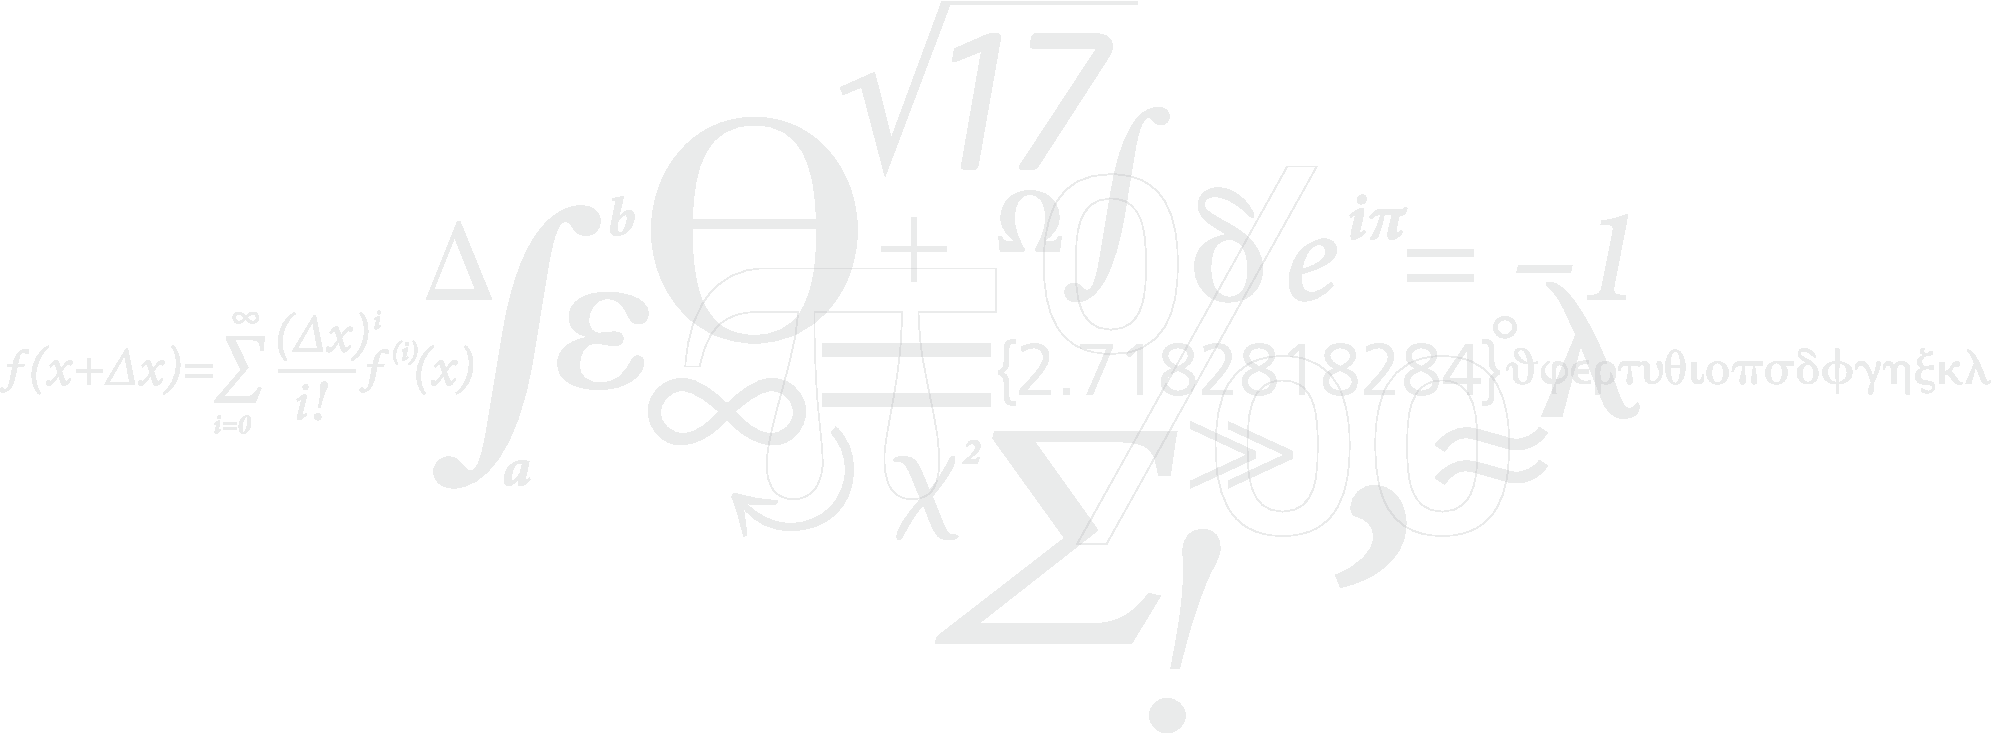
\includegraphics[trim=130mm 0 0 0,width=0.9\textwidth]{DTU-frise-SH-15}
                \vspace*{2.5cm}
            }
        }
    }
}

% This is a double sided book. If there is a last empty page lets use it for some fun e.g. the frieze.
% NB: For a fully functional hack the \clearpage used in \include does some odd thinks with the sequence numbering. Thefore use \input instead of \include at the end of the book. If bibliography is used at last everything should be ok.
\makeatletter
% Adjust so gatherings is allowd for single sheets too! (hacking functions in memoir.dtx)
\patchcmd{\leavespergathering}{\ifnum\@memcnta<\tw@}{\ifnum\@memcnta<\@ne}{
    \leavespergathering{1}
    % Insert the frieze
    \patchcmd{\@memensuresigpages}{\repeat}{\repeat\frieze}{}{}
}{}
\makeatother

%%%%%%%%%%%%%%%%%%%%% PACKAGES %%%%%%%%%%%%%%%%%%%%%%%%%%%%%%
\usepackage{epigraph}
\usepackage{hyperref}      % To make the acronyms clickable. All the other
                           % hyperref are provided by memoir
\usepackage{lipsum}        % To generate Lorem Ipsum filling text
\usepackage{algpseudocode} % For algorithm environment
\usepackage{physics}      % For \Re \Im as Re() Im() and tons of operators,
                          % partial derivatives and more
\usepackage[binary-units]{siunitx}      % Properly type SI units
\usepackage{etoolbox}     % Used to alter the \chapter command to reset acronyms

\usepackage{xargs}        % To define commands with more than one optional value
\usepackage{mathtools}    % For ceiling and floor operator
\usepackage{amsfonts}     % For \mathbb{}
\usepackage{amssymb}      % \triangeq
\usepackage{amsmath}
\usepackage{xr}           % Cross reference among documents (useful for the supplementary information)
\usepackage[printonlyused]{acronym} % Allows to define acronyms (nolist = do not create a list of acronyms)
\usepackage{dblfloatfix}  % To enable figures at the bottom of page
\usepackage{stackengine}  % Allow multiple diacritcs
\usepackage{bigints}      % Big integrals
\usepackage{steinmetz}    % For phase symbol (\phase)
\usepackage[export]{adjustbox}    % adjustbox for rotating tables, aligning \includegraphics at top valign=t
\usepackage[]{todonotes}
\usepackage{xpatch}       % To patch latex commands
\usepackage{ifdraft}
\usepackage{tabu}         % Better tables
%\usepackage[toc]{glossaries}
\usepackage{enumitem}  % To customize enumerate environment (see Symbols.tex)

%\usepackage{cleveref}    % \ref will write Equation (1), Figure 1
\usepackage{environ}      % To define the extendedthesis env


\usepackage{makecell}    % Allows line break within a table cell
%\usepackage{subfig}

%\usepackage[markup=underlined,final]{changes} %% Use "final" option to remove all
%\usepackage{ifthen}      & To use \ifthenelse statement. This package is already imported by the template in this case.

%%%%%%%%%%%%% PACKAGES RELATED DEFINITIONS %%%%%%%%%%%%%%%%%%
% mathtools
\DeclarePairedDelimiter\ceil{\lceil}{\rceil}
\DeclarePairedDelimiter\floor{\lfloor}{\rfloor}

\sisetup{per-mode=symbol}       % Display SI units as dB/km
                                % Accepts 'reciprocal' (dB km^-1) 'fraction' (\frac)

% siuntix
\DeclareSIUnit{\dBm}{dBm}

% etoobox/acronym
\preto\chapter\acresetall       % Prepend \acresetall to the command \chapter
                                % \acresetall re-expand acronyms after this command

% Create a new environment to put things to extende the thesis
\newif\ifextendedthesis
\extendedthesisfalse            % Set to false to hide the extensions of the thesis
\NewEnviron{extendedthesis}{\ifextendedthesis\color{gray}\BODY\fi}

% Full line comment for algorithms
\algnewcommand{\LineComment}[1]{\State \(\triangleright\) #1}

% Patch to acronym to avoid multiple defined labels when using cleverref?
\makeatletter
\newcommand*{\org@overidelabel}{}
\let\org@overridelabel\@verridelabel
\@ifpackagelater{acronym}{2015/03/21}{% v1.41
  \renewcommand*{\@verridelabel}[1]{%
    \@bsphack
    \protected@write\@auxout{}{\string\AC@undonewlabel{#1@cref}}%
    \org@overridelabel{#1}%
    \@esphack
  }%
}{% older versions
  \renewcommand*{\@verridelabel}[1]{%
    \@bsphack
    \protected@write\@auxout{}{\string\undonewlabel{#1@cref}}%
    \org@overridelabel{#1}%
    \@esphack
  }%
}
\makeatother

% biblatex: Avoid long list of citations to be breaked by a newline in the middle
\renewcommand*{\multicitedelim}{\addcomma\nobreakspace}
% FIX: Avoid newline between last word and citation list

% Make the (a) be centered in a figure if no text is provided (e.g. \subtop[]{ )
\makeatletter
\def\@memsubfig[#1]{%
  \@ifnextchar [%
    {\@memsubfloat{sub\@captype}[#1]}%
    {\@memsubfloat{sub\@captype}[\@empty #1][#1\unskip]}}
\makeatother

% Biblatex fix - Allow to write $\pi$ instead of {$\pi%} in .bib file
\makeatletter
\def\blx@mksc@init{%
  \blx@mkcp@init
  \def\blx@mkcp@nil{\noexpand\blx@mkcp@nil\noexpand}%
  \def\i{\blx@mkcp@nil\i}\def\j{\blx@mkcp@nil\j}%
  \def\do##1{%
    \ifx##1\relax
    \else
      \def##1{\blx@mkcp@nil##1}%
      \expandafter\do
    \fi}%
  \expandafter\do\@uclclist\relax
  \let\(=$\let\)=$}

\def\blx@mksc@eval{%
  \ifx\@let@token\blx@mksc@end
    \expandafter\blx@mksc@end
  \fi
  \ifx\@let@token\bgroup
    \expandafter\blx@mksc@group
  \fi
  \ifx\@let@token\@sptoken
    \expandafter\blx@mksc@space
  \fi
  \ifx\@let@token\blx@mkcp@nil
    \expandafter\blx@mksc@getone
  \fi
  \ifx\@let@token\blx@mkcp@iec
    \expandafter\blx@mksc@getiec
  \fi
  \ifx\@let@token\blx@mkcp@bbl
    \expandafter\blx@mksc@gettwo
  \fi
  \ifx\@let@token\blx@mkcp@sgl
    \expandafter\blx@mksc@gettwo
  \fi
  \ifx\@let@token\blx@mkcp@dbl
    \expandafter\blx@mksc@getthree
  \fi
  \ifx\@let@token$%
    \expandafter\blx@mksc@getmath
  \fi
  \if\noexpand\@let@token\relax
    \expandafter\blx@mksc@cs
  \fi
  \blx@mksc@other}

\def\blx@mksc@getmath#1\blx@mksc@other$#2${\blx@mksc@other{{$#2$}}}
\makeatother

% Patch acronym package to allow hypenation of first acronym word
\makeatletter
\patchcmd\@acf{\AC@acl}{\AC@foo}{}{}
\patchcmd\@acf{\AC@acl}{\AC@foo}{}{}
\patchcmd\@acf{\AC@foo}{\hskip\z@\AC@acl}{}{}
\patchcmd\@acf{\AC@foo}{\hskip\z@\AC@acl}{}{}
\makeatother


% Ignore badboxes of less than 3pt
\hfuzz=3pt
%\vfuzz

%!TEX root = ../Thesis.tex

% Text fonts (http://www.macfreek.nl/memory/Fonts_in_LaTeX)
% Install fonts from /usr/local/texlive/<version>/texmf-dist/fonts/opentype/public
\usepackage{fontspec}

% Sans-serif font
\setsansfont[
    Ligatures=TeX,
    Extension=.otf,
    UprightFont=*-regular,
    BoldFont=*-bold,
    ItalicFont=*-italic,
    BoldItalicFont=*-bolditalic,
    %SlantedFont=,
    %BoldSlantedFont=,
    %SmallCapsFont=
    Scale=0.8      % Adjustmens when using math in sections
]{texgyreadventor}
%\setsansfont[Ligatures=TeX]{Neo Sans Intel}    % Neo Sans Intel – Like DTU font but more symbols
%\setsansfont[
%    Ligatures=TeX,
%    Scale=0.8
%]{NeoSans}           % NeoSans – DTU font (missing `+' symbols and other)
%\setsansfont[Ligatures=TeX]{CMU Sans Serif}    % Computer Modern Unicode font
%\setsansfont[Ligatures=TeX]{Latin Modern Sans} % Latin Modern Sans serif font

% Use this for more convienent sans serif font in math mode.
%\setmathsf{Latin Modern Sans}


%!TEX root = ../Thesis.tex

% Content specific packages.

\usepackage{blindtext}
\usepackage{algorithm}
\usepackage{algpseudocode}
%\usepackage{pgfplots}                 % Plot tools
%\usetikzlibrary{
%    arrows,
%    matrix,
%    positioning,
%    shapes,
%    topaths,
%}
%\pgfplotsset{compat=1.7}

% Listings
\lstset{
    basicstyle=\footnotesize\ttfamily,% the size of the fonts that are used for the code
    breakatwhitespace=false,          % sets if automatic breaks should only happen at whitespace
    breaklines=true,                  % sets automatic line breaking
    captionpos=b,                     % sets the caption-position to bottom
    commentstyle=\color{s14a},        % comment style
    deletekeywords={},                % if you want to delete keywords from the given language
    escapeinside={\%*}{*)},           % if you want to add LaTeX within your code
    frame=single,                     % adds a frame around the code
    keywordstyle=\bfseries\ttfamily\color{s09}, % keyword style
    language=Python,                  % the language of the code
    morekeywords={*,...},             % if you want to add more keywords to the set
    numbers=left,                     % where to put the line-numbers; possible values are (none, left, right)
    numbersep=5pt,                    % how far the line-numbers are from the code
    numberstyle=\sffamily\tiny\color{dtugray}, % the style that is used for the line-numbers
    rulecolor=\color{dtugray},        % if not set, the frame-color may be changed on line-breaks within not-black text (e.g. comments (green here))
    showspaces=false,                 % show spaces everywhere adding particular underscores; it overrides 'showstringspaces'
    showstringspaces=false,           % underline spaces within strings only
    showtabs=false,                   % show tabs within strings adding particular underscores
    stepnumber=1,                     % the step between two line-numbers. If it's 1, each line will be numbered
    stringstyle=\color{s07},          % string literal style
    tabsize=2,                        % sets default tabsize to 2 spaces
    title=\lstname,                   % show the filename of files included with \lstinputlisting; also try caption instead of title
}


%%%%%%%%%%%%%%%%%%%% ABBREVIATIONS %%%%%%%%%%%%%%%%%%%%%%%%%%
% Units
\newcommand{\gbaud}{GBd}

% Terms
\newcommand{\scatcoef}{scattering coefficients}
\newcommand{\zs}{Zakharov-Shabat}
\newcommand{\mz}{Mach-Zehnder}
\newcommand{\nfdmsymbol}{\ac{NFDM}-symbol}

%%%%%%%%%%%%%%%%%%%%% COMMANDS %%%%%%%%%%%%%%%%%%%%%%%%%%%%%%
% Latex
\newcommand{\figref}[1]{\figurename~\ref{#1}}       % Figure reference as 'Figure 1'
\newcommand{\tabref}[1]{\tablename~\ref{#1}}        % Table reference as 'Table 1'
\newcommand{\chref}[1]{\chaptername~\ref{#1}}       % chapter reference as 'Table 1'
\newcommand{\codeword}[1]{\texttt{{#1}}}            % Italiic for pieces of code

% Figures
\newcommand{\figuresvspace}{\vspace{0.2cm}}
\newcommand{\figuresvspacenl}{\vspace{0.2cm}\newline}

% General math
\newcommand{\RR}{\mathbb{R}}                % Set of real numbers
\newcommand{\CC}{\mathbb{C}}                % Set of complex numbers
\newcommand{\iunit}{i}                      % Imaginary unit

% Operators
\DeclareMathOperator*{\expectation}{E}      % Expectation
\DeclareMathOperator*{\argmin}{argmin}      % argmin
\DeclareMathOperator*{\argmax}{argmax}      % argmax
\DeclareMathOperator*{\nmse}{NMSE}          % Normalized mean squared error
\DeclareMathOperator*{\papr}{PAPR}          % Peak-to-average power ratio
\DeclareMathOperator*{\osnr}{OSNR}          % Optical signal-to-noise ratio
\DeclareMathOperator*{\snr}{SNR}            % Signal-to-noise ratio
\DeclareMathOperator*{\diagmatr}{diag}      % Diagonal matrix inline


\newcommand{\matr}[1]{\mathbf{#1}}

% NLSE/Manakov
\newcommand{\ttm}{\tau}                     % Time
\newcommand{\ssp}{\ell}                     % Space
\newcommand{\fld}[1][]{E_{#1}}              % Electrical field/signal
\newcommand{\flds}[1][]{\fld[#1]            % Field/signal  with time coordinate
                (\ttm)}
\newcommand{\nttm}{t}                       % Normalized time
\newcommand{\nssp}{z}                       % Normalized space
\newcommand{\nfld}[1][]{q_{#1}}             % Normalized field/signal
\newcommand{\nflds}[1][]{\nfld[#1]          % Normalized field/signal  with time coordinate
                (\nttm)}
\newcommand{\nflddig}[1][]{\nfld[#1]          % Normalized field/signal  with discrete time coordinate
                (\nttm_n)}
\newcommand{\nfldl}[1][]{\nfld[#1]          % Normalized field/signal  with coordinates
                (\nttm, \nssp)}
\newcommand{\loss}{\alpha}                  % Loss coefficient (alpha)
\newcommand{\dispersion}{\beta_2}           % Dispersion coefficient (beta2)
\newcommand{\nonlinfact}{\gamma}            % Nonlinear coefficient (gamma)
\newcommand{\fiberl}{L}                     %  Fiber length
\newcommand{\spanl}{L_{s}}                  %  Span length
\newcommand{\nspans}{N_s}                   %  Number of spans

% NFDM system
\newcommand{\Rs}{$R_{s}$}                   % Symbol rate
\newcommand{\Ts}{$T_{s}$}                   % Symbol period
\newcommand{\Tsi}[1]{$T_{s,#1}$}            % Symbol period i-th
\newcommandx{\sTx}[2][1=,2=]{\ifthenelse{   % Transmitted waveform
  \equal{#1}{}}
    {\fld[Tx](\ttm_{#2})}
    {\fld[Tx,#1](\ttm_{#2})}
  }
\newcommandx{\sRx}[2][1=,2=]{\ifthenelse{   % Received waveform
  \equal{#1}{}}
    {\fld[Rx](\ttm_{#2})}
    {\fld[Rx,#1](\ttm_{#2})}
  }
\newcommand{\sdTx}[1][]{\sTx[#1][n]}          % Transmitted digital waveform
\newcommand{\sdRx}[1][]{\sRx[#1][n]}          % Received digital waveform
\newcommand{\nfdmsymtx}{\{\eig[1], \dots, \eig[N], \nftb[][1], \dots, \nftb[][N]\}}
\newcommand{\nfdmsymrx}{{\{\eigest[1], \dots, \eigest[N], \nftbest[][1], \dots, \nftbest[][N]\}}}
% Other optical terms
\newcommand{\phnoise}{\sigma_n}             % Phase noise variance
\newcommand{\asenoise}{n}                   % ASE noise term

% NFT
\newcommand{\nftcvL}{\mathcal{L}}           % NFT characteristic length
\newcommand{\To}{$T_{0}$}                   % NFT characteristic time

\newcommand{\eig}[1][]{\lambda_{#1}}                  % Eigenvalue [1 = subscript index]
\newcommand{\eigf}[1][]{v_{#1}}                       % Eigenfunction [1 = subscript index]
\newcommand{\vecv}{v}  % Obsolete, use eigf           % Solution ZS problem
\newcommand{\nfta}[1][]{a(\eig[#1])}                  % NFT coefficient 'a' [1 = subscript index]
\newcommand{\nftaderiv}[1][]{a'(\eig[#1])}            % NFT coefficient 'a1' [1 = subscript index]
\newcommandx{\nftb}[2][1=, 2=]{\ifthenelse{%          % NFT coefficient 'b'[1 = mode index, 2 = subscript index]
  \equal{#2}{}}{b_{#1}(\eig)}{b_{#1}(\eig[#2])}}
\newcommand{\cnft}[1][]{\ifthenelse{                  % NFT continuous spectrum [1 = subscript index]
  \equal{#1}{}}{Q_{c}(\eig)}{Q_{c,#1}(\eig)}}
\newcommand{\dnft}[1][]{\ifthenelse{                  % NFT discrete spectrum [1 = subscript index]
  \equal{#1}{}}{Q_{d}(\eig)}{Q_{d}(\eig[#1])}}
\newcommand{\cnftsp}[1][]{Q_{c}(\eig}                 % NFT continuous spectrum with space for space var
\newcommand{\dnftsp}[1][]{\ifthenelse{
  \equal{#1}{}}{Q_{d}(\eig}{Q_{d}(\eig[#1]}}   % NFT discrete spectrum with space for space var
\newcommand{\nftH}[1][]{e^{-4\iunit\eig[#1]^2\nssp}}         % NFT spectrum space evolution / Channel transfer function
\newcommandx{\nftInvH}[2][1=, 2=]{e^{4\iunit\eig[#1]^2#2}}       % Inverse NFT spectrum space evolution (z = 1) / Inverse channel transfer function
\newcommand{\nEig}{N}                                 % Number of discrete eigenvalues
\newcommand{\bitsperblock}{d}
% Estimated at the reciever
\newcommand{\eigest}[1][]{\ifthenelse{                % Eigenvalue [1 = subscript index]
  \equal{#1}{}}
    {{\widetilde{\lambda}}}
    {{\widetilde{\lambda}_#1}}
  }
\newcommandx{\nftbest}[2][1=, 2=]{\ifthenelse{        % NFT coefficient 'b'[1 = mode index, 2 = subscript index]
  \equal{#2}{}}
    {\widetilde{b_{#1}}(\eigest)}
    {\widetilde{b_{#1}}(\eigest[#2])}
  }
\newcommand{\cnftest}[1][]{\ifthenelse{                  % NFT continuous spectrum [1 = subscript index]
  \equal{#1}{}}
    {\widehat{Q}_{c}(\eig)}
    {\widehat{Q}_{c, #1}(\lambda)}
  }
% Conjugate versions
\newcommand{\nftaconj}[1][]{\bar{a}(\eig[#1])}        % NFT coefficient 'a' conjugate [1 = subscript index]
\newcommandx{\nftbconj}[2][1=, 2=]{\ifthenelse{       % NFT coefficient 'b' conjugate [1 = mode index, 2 = subscript index]
  \equal{#2}{}}
    {\bar{b}_{#1}(\eig)}
    {\bar{b}_{#1}(\eig[#2])}
  }
% Jost solutions
\newcommand{\jost}[1][]{\phi_{#1}(t,\eig)}            % Jost solution generic
\newcommandx{\jostp}[2][1=, 2=]{\ifthenelse{                 % Jost solution p [1 = component index, 2 = eigenvalue index]
  \equal{#2}{}}
    {\phi^{P}_{#1}(t,\eig)}
    {\phi^{P}_{#1}(t,\eig[#2])}
  }
\newcommandx{\jostn}[2][1=, 2=]{\ifthenelse{                 % Jost solution n [1 = component index, 2 = eigenvalue index]
  \equal{#2}{}}
    {\phi^{N}_{#1}(t,\eig)}
    {\phi^{N}_{#1}(t,\eig[#2])}
  }
\newcommand{\jostpconj}[1][]{\bar{\phi}^{P}_{#1}      % Jost solution p conjugate
            (t,\eig)}
\newcommand{\jostnconj}[1][]{\bar{\phi}^{N}_{#1}      % Jost solution n conjugate
            (t,\eig)}
\newcommand{\jostpshrt}[1][]{\phi^{P}_{#1}}           % Jost solution p (short notation)
\newcommand{\jostnshrt}[1][]{\phi^{N}_{#1}}           % Jost solution n (short notation)
\newcommand{\jostpconjshrt}[1][]{\bar{\phi}^{P}_{#1}} % Jost solution p conjugate (short notation)
\newcommand{\jostnconjshrt}[1][]{\bar{\phi}^{N}_{#1}} % Jost solution n conjugate (short notation)

% Darboux
\newcommand{\nfldsmod}[1][]{\hat{q}_{#1}             % Normalized field/signal  with time coordinate
                (\nttm)}

\newcommand{\auxsol}{\bar{v}}           % Darboux transform auxiliary solution
\newcommand{\auxsolmat}{\Theta} % Darboux transform auxiliary solution matrix

% NFT math relateed quantities
\newcommand{\wron}[2]{W(#1, #2)} % Wronskian

% NFT math relateed quantities - Single pol
% \newcommand{\vv}{\begin{pmatrix} \psi_1\\ \psi_2\end{pmatrix}} % Obsolete
% \newcommand{\vvt}{\renewcommand*{\arraystretch}{1.2}\begin{pmatrix} \frac{\partial\psi_1}{\partial\tau}\\ % Obsolete
% \frac{\partial\psi_2}{\partial\tau}\end{pmatrix}}
\newcommand{\matL}{\boldsymbol{L}}
\newcommand{\matP}{\boldsymbol{P}}
\newcommand{\matM}{\boldsymbol{M}}
\newcommand{\matPfull}{\begin{pmatrix} -j\eig & q(t) \\ -q(t)^* & j\eig \end{pmatrix}}

% NFT math relateed quantities - Dual pol
\newcommand{\mzssol}[1][]{v_{#1}}                        % Vector solution ofthe ZSP [1 = component number] (Was \dv)
% \newcommand{\dvv}{\begin{pmatrix} % Obsolete
%         \psi_1\\ \psi_2\\ \psi_3\end{pmatrix}} % Obsolete
% \newcommand{\dvvt}{\renewcommand*{\arraystretch}
%         {1.2}\begin{pmatrix} \frac{\partial\psi_1}
%         {\partial\tau}\\
% \frac{\partial\psi_2}{\partial\tau}\end{pmatrix}}

% Forward backward method
\newcommand{\psisol}[1][]{\psi_{#1}}               % Solution of the ZSP after the change of variable [1 = component number]
\newcommand{\fbw}[1][]{w_{#1}}                     % Solution of the ZSP after the change of variable [1 = component number]
\newcommand{\fbu}[1][]{u_{#1}}                     % Solution of the ZSP after the change of variable [1 = component number]

\newcommand{\tjostp}[1][]{\psi^{P}_{#1}(t,\eig)}   % Transformed Jost solution p
\newcommand{\tjostn}[1][]{\psi^{N}_{#1}(t,\eig)}   % Transformed Jost solution n
\newcommand{\tjostpshrt}[1][]{\psi^{P}_{#1}}       % Transformed Jost solution p (short notation)
\newcommand{\tjostnshrt}[1][]{\psi^{N}_{#1}}       % Transformed Jost solution n (short notation)

% From NFT tutorial paper (should be removed and not used)
\newcommand{\wrong}[1]{{\color{red}#1}}
\newcommand{\ms}[1]{\mathds{#1}}
\newcommand{\Ex}{\ms{E}}
\newcommand{\Ns}{n_{\tnr{s}}}
\newcommand{\tnr}[1]{{\textnormal{#1}}}
\newcommand{\ld}{\ldots}
\newcommand{\set}[1]{\{#1\}}
\newcommand{\mcXkb}{\mathcal{X}_{k}^{b}}
\newcommand{\mcXko}{\mathcal{X}_{k}^{1}}
\newcommand{\mcXkz}{\mathcal{X}_{k}^{0}}
\newcommand{\mcX}{\mathcal{X}}

% Command to reference a figure inset
\newcommand{\insetref}[1]{(\textbf{#1})}

%%%%%%%%%%%%%%%%%%%%% COMMANDS RENEWED %%%%%%%%%%%%%%%%%%%%%%

% Compact matix
\newcommand{\compactmat}{\renewcommand                % Reduce the vertical space inside matrices
        {\arraystretch}{1}}

% Equation number with S1 style (for supplementary information)
% \renewcommand{\theequation}{S.\arabic{equation}}

% System of equations with a single equation number
\newenvironment{nalign}{                              % Align environment with a single equation number for multiple equations
    \begin{equation}
    \begin{aligned}
}{
    \end{aligned}
    \end{equation}
    \ignorespacesafterend
}


% Make my name bold (needs to be annotated in the bibliography)
\renewcommand*{\mkbibnamegiven}[1]{%
\ifitemannotation{simonegaiarin}
{\textbf{#1}}
{#1}}

\renewcommand*{\mkbibnamefamily}[1]{%
\ifitemannotation{simonegaiarin}
{\textbf{#1}}
{#1}}

\newcommand{\symb}[1]{\item[${#1}$]}
\newcommand{\symbt}[1]{\item[{#1}]}

\addbibresource{bibliography/Bibliography.bib}

\begin{document}
\prefrontmatter
%!TEX root = ../Thesis.tex
\thispagestyle{empty}             % No page numbers
\calccentering{\unitlength}
\begin{adjustwidth*}{\unitlength}{-\unitlength}
    \begin{adjustwidth}{-0.5cm}{-0.5cm}
        \sffamily
        \begin{flushright}
            \thesistypeabbr{} Thesis\\*[0cm]
            \thesistype{}\\
        \end{flushright}
        \vspace*{\fill}
        \noindent
        
\includegraphics[width=0.75\textwidth]{DTU-Fotonik-B-UK}\\*[0.5cm]
        \HUGE \thesistitle{}\\*[0.2cm]
        \Huge \thesissubtitle{}\\*[1.2cm]
        \parbox[b]{0.5\linewidth}{%
            \LARGE
            \thesisauthor{}\\*[1.2cm]
            \Large
            \thesislocation{} \the\year
        }
        \hfill
\includegraphics[scale=0.7]{DTU-logo-CMYK}
    \end{adjustwidth}
\end{adjustwidth*}
\normalfont
\normalsize

\cleartoevenpage
%!TEX root = ../Thesis.tex
\thispagestyle{empty} % No page numbers
\frieze
\vspace*{\fill}
\noindent
\sffamily
\small
\textbf{DTU Fotonik}\\
\textbf{Department of Photonics Engineering}\\
\textbf{Technical University of Denmark}\\
\\
Ørsteds Plads\\
Building 343\\
2800 Kongens Lyngby, Denmark\\
Phone +45 4525 6352\\
www.fotonik.dtu.dk\\
\normalsize
\normalfont
\vspace*{2.5cm}

\clearforchapter


\frontmatter
\chapter{Abstract}



New services and applications are causing an exponential increase in internet traffic.  In a few years, current fiber optic communication system infrastructure will not be able to meet this demand because fiber nonlinearity dramatically limits the information transmission rate. Eigenvalue communication is considered an emerging paradigm in fiber optics communications that could potentially overcome these limitations. It relies on a mathematical technique called ``inverse scattering transform'' or ``\ac{NFT}'' to exploit the ``hidden'' linearity of the \acl{NLSE} as the master model for signal propagation in an optical fiber.
One of the rapidly evolving \ac{NFT}-based communication techniques is called \ac{NFDM}.
% This modulation method encodes the data on the  nonlinear spectrum associated by the NFT to a time domain signal.
Being still in its infancy, \ac{NFDM} systems still have some practical limitations. One of these limitations is the lack of polarization division multiplexing.

The results presented in this thesis address this problem.
% First the theory of single polarization NFT is reviewed, and a generalized channel model that accounts for fiber loss and noise is introduced. The applicability of the NFT over this channel is evaluated through numerical simulations, demonstrating that even using this approximate model the nonlinear spectrum is less distorted by nonlinearities when compared to the linear Fourier spectrum.
First the structure of an \ac{NFDM} system using the discrete nonlinear spectrum is described. The particular design aspects of this system are then discussed in details.

Subsequently, the theoretical tools describing the NFT for the Manakov system describing the evolution of a dual polarization signal in a \acl{SMF}  are presented. Using these tools the discrete \ac{NFDM} system is extended to the the dual polarization case.
Finally, the results of the first experimental transmission of a dual polarization \ac{NFDM} system are presented. A transmission of up to 373.5 km with bit error rate less than the hard-decision forward error correction threshold has been achieved.

The results presented demonstrate that dual-polarization \ac{NFT} can work in practice and enable an increased spectral efficiency in \ac{NFT}-based communication systems, which are currently based on single polarization channels.


\clearforchapter
%!TEX root = ../Thesis.tex
\chapter{Preface}

I'll write this

This xxx thesis was prepared at the department of Applied Mathematics and Computer Science at the Technical University of Denmark in fulfillment of the requirements for acquiring a yyy degree in zzz.

\vfill

{
\centering
    \thesislocation{}, \today\\[1cm]
    \hspace{3cm}
\includegraphics[scale=0.4]{Signature}\\[1cm]
\begin{flushright}
    \thesisauthor{}
\end{flushright}
}

\clearforchapter
%!TEX root = ../Thesis.tex
\chapter{Acknowledgements}
Alex Alvarado
Oskars and Xiaodan
ICONE people


\clearforchapter
% Epigraph
\vspace*{0.2\textheight}
\renewcommand{\epigraphsize}{\large}
\setlength{\epigraphwidth}{0.8\textwidth}
\setlength{\epigraphrule}{0pt}
%\epigraph{\textit{Science is like sex: sometimes something useful comes out, \\ but that is not the reason we are doing it.}}{- Richard Feynman}

\epigraph{\textit{Some like to understand what they believe in. \\Others like to believe in what they understand.}}{- Stanisław Lec}





\clearforchapter
%%%%% DON'T EDIT MANUALLY THE
\chapter{Ph.D. Publications}
%\fancyhead[RE]{\bf Ph.D. Publications}

The following publications have resulted from this Ph.D. project.

% !!NOTE!! Delete .aux files when changing the options of biblatex
% Usually it is required if the sorting or numbers are wrong

% sorting=ydnt  -  By years descending
% labelprefix   -  Add prefix to citation number
% keyword       -  Print only references matching that keyboard
% heading=subbibliography  -  Print bibliography as section not as chapter
% resetnumbers  -  Start counting from 1 in the sectioin.
%                  Requires global flag defernumbers
% title         -  Custom title for the section

\begin{refcontext}[sorting=ydnt, labelprefix=J]
    \nocite{ozolins2017100,pang2017experimental,da2016combined} % Not cited in the text
    % \nocite{Rasmus2018} % Rasmus paper to be submitted
    \nobibintoc % Prevent the section title to appear in the bibliography
                % subbibliography should already not appear, seems a bug
    \printbibliography[keyword=GaiarinJournals,heading=subbibliography,
    title={Articles in peer-reviewed journals}]
\end{refcontext}


\begin{refcontext}[sorting=ydnt,labelprefix=C]
    \nocite{Rasmus2017,pang2016evaluation,ozolins2016100,gaiarin2016high,popov2016ultra}
    \nocite{GaiarinECOC17} % Can remove this later
    \nobibintoc
    \printbibliography[keyword=GaiarinConferences,heading=subbibliography,
    resetnumbers=true,
    title={Contributions to international peer-reviewed conferences}]
\end{refcontext}

\clearforchapter
\tableofcontents*
\clearforchapter
\chapter{Acronyms}

% - Passing the longest acronym as parameter to the environment allows
%   aligning properly the acronyms in the list of acronyms
% - The acronyms needs to be alphabetically sorted manually here
% - The package hyperref is necessary to make the acronyms clickable
\begin{acronym}[DP-NFDM]
\acro{ADC}{analog-to-digital converter}
\acro{ADM}{add-drop multiplexer}
\acro{ASE}{amplified spontaneous emission}
\acro{AIR}{achievable information rate}
\acro{AKNS}{Ablowitz-Kaup-Newell-Segur}
\acro{AWG}{arbitrary waveform generator}
\acro{AWGN}{additive white Gaussian noise}
\acro{B2B}{back-to-back}
\acro{BER}{bit error rate}
\acro{BPD}{balanced photodetector}
\acro{BPS}{blind phase search}
\acro{DAC}{digital-to-analog converter}
\acro{DC}{direct current}
\acro{DCF}{dispersion compensating fiber}
\acro{DBP}{digital back-propagation}
\acro{DFT}{discrete Fourier transform}
\acro{DP-NFDM}{dual-polarization nonlinear frequency division multiplexing}
\acro{DSO}{digital storage oscilloscope}
\acro{DSP}{digital signal processing}
\acro{DT}{Darboux transformation}
\acro{EDC}{electrical dispersion compensation}
\acro{EDFA}{erbium-doped fiber amplifier}
\acro{ENOB}{effective number of bits}
\acro{FEC}{forward error correction}
\acro{FFT}{fast Fourier transform}
\acro{FL}{fiber laser}
\acro{FWHM}{full-width half-maximum}
\acro{FWM}{four-wave mixing}
\acro{GLM}{Gelfand-Levitan-Marchenko}
\acro{GVD}{group velocity dispersion}
\acro{HD-FEC}{hard-decision forward error correction}
\acro{I}{in-phase}
\acro{IFFT}{inverse fast Fourier transform}
\acro{INFT}{inverse nonlinear Fourier transform}
\acro{ISI}{inter-symbol interference}
\acro{IST}{inverse scattering transform}
\acro{IVP}{initial value problem}
\acro{LO}{local oscillator}
\acro{LPA}{lossless path-averaged}
\acro{MS}{Manakov system}
\acro{MAP}{maximum a posteriori}
\acro{ML}{maximum likelihood}
\acro{MZM}{Mach-Zehnder modulator}
\acro{MZSP}{Manakov-Zakharov-Shabat spectral problem}
\acro{NFDM}{nonlinear frequency division multiplexing}
\acro{NFT}{nonlinear Fourier transform}
\acro{NIS}{nonlinear inverse synthesis}
\acro{NLSE}{nonlinear Schr\"odinger equation}
\acro{NMSE}{normalized mean squared error}
\acro{OBPF}{optical band pass filter}
\acro{ODE}{ordinary differential equation}
\acro{OFDM}{orthogonal frequency-division multiplexing}
\acro{OPC}{optical phase conjugation}
\acro{OSNR}{optical signal-to-noise ratio}
\acro{PAPR}{peak-to-average power ratio}
\acro{PC}{polarization controller}
\acro{PDE}{partial differential equation}
\acro{PMD}{polarization mode dispersion}
\acro{ppm}{parts-per-million}
\acro{PSK}{phase-shift keying}
\acro{Q}{quadrature}
\acro{QAM}{quadrature amplitude modulation}
\acro{QPSK}{quadrature phase-shift keying}
\acro{SDM}{space-division multiplexing}
\acro{SMF}{single mode fiber}
\acro{SNR}{signal-to-noise ratio}
\acro{S/P}{serial-to-parallel}
\acro{SPM}{self-phase modulation}
\acro{SSFM}{split-step Fourier method}
\acro{WDM}{wavelength-division multiplexing}
\acro{XPM}{cross-phase modulation}
\acro{ZSP}{Zakharov-Shabat spectral problem}
\end{acronym}

\clearforchapter
%\printglossaries
\chapter{List of frequently used symbols}

\begin{enumerate}[wide=0pt, labelwidth=4em, align=left]

% Lower case
% a
\symb{\nfta} Scattering coefficient
\symb{\nftaconj}  Scattering coefficient
% b
\symb{\nftb} Scattering coefficient
\symb{\nftbconj}  Scattering coefficient
\symb{\nftbest}  Scattering coefficient estimated at the receiver
% d
\symb{d} Bits per data frame (\acs{NFDM} symbol)
% k
\symb{k} Bits per eigenvalue
% l
\symb{\ssp}  Space coordinate
% q
\symb{\nfldl}  Normalized complex envelope of the electric field
\symb{\nfldsmod}  $\nfld(\nttm, 0)$ modified by the \acs{DT}
% r
\symb{r_1, r_2 } Radius of the constellations associated to the eigenvalues $\eig[1], \eig[2]$
\symb{\matr{r}} Digital received \acs{NFDM}-symbol
% s
\symb{\matr{s}} Digital transmitted \acs{NFDM}-symbol
% t
\symb{\nttm}  Normalized time coordinate
% u
\symb{\fbu}  $\jostn$ propagated forward  in the forward-backward method
% v
\symb{\eigf}  Solution of the \acs{ZSP} / \acs{MZSP}
\symb{\auxsol}  Darboux transformation auxiliary solution
% w
\symb{\fbw}  $\jostn$ propagated backward in the forward-backward method
% z
\symb{\nssp}  Normalized space coordinate

% Upper case
% C
\symb{C_r} Reference $\nftb[][i]$ constellation for optimization
% D
\symb{D} Fiber dispersion parameter
% E
\symb{\fld(\ttm,\ssp)}  Complex envelope of the electric field
\symb{\sRx} Received optical waveform
\symb{\sdRx}  Received digital waveform
\symb{\sTx}  Transmitted optical waveform
\symb{\sdTx}  Transmitted digital waveform
% G
\symb{\matr{G}_0} Darboux transformation matrix
% K
\symb{K} Number of samples of the time domain signal $\nflds$
% L
\symb{\fiberl}   Fiber link length
\symb{L_d} Dispersion length
\symb{\spanl} Fiber span length
\symb{\matL} Lax operator
\symb{\nftcvL}  Nonlinear Schr\"odinger equation length normalization factor
% M
\symb{M} Constellation order
\symb{\matM} Lax space-evolution matrix
% N
\symb{\nEig} Number of eigenvalues
\symb{\nspans} Number of spans constituting a fiber link
% P
\symb{P} Nonlinear Schr\"odinger equation power normalization factor
\symb{P_{tx}} Average power of the transmitted optical signal
\symb{\matP} Lax time-evolution matrix
% Q
\symb{\cnftsp,\nssp)}  Continuous spectral amplitude
\symb{\cnftest}  Continuous spectral amplitude estimated at the receiver
\symb{\dnftsp,\nssp)}  Discrete  spectral amplitude
% R
\symbt{\Rs}  Symbol rate
% T
\symb{T} Total time duration of the transmitted signal $\sTx$
\symb{T_b} Bit period
\symbt{\Ts}  Symbol period
\symbt{\To}  Nonlinear Schr\"odinger equation time-normalization factor
% V
\symb{V_{\pi}} \acl{MZM} half-wave voltage
% W
\symb{W} Bandwidth containing 99\% of the power of the signal


% Greek lower case
% α
\symb{\loss} Fiber-loss parameter
% β
\symb{\dispersion} Fiber \acl{GVD}
% γ
\symb{\nonlinfact} Fiber nonlinear parameter
\symb{\bar{\nonlinfact}} Fiber nonlinear parameter averaged over one span length
% θ
\symb{\theta_e} Relative angle between constellations for the two eigenvalues
\symb{\theta_p} Relative angle between constellations for the two polarizations
% λ
\symb{\eig} Eigenvalue
\symb{\eigest}  Eigenvalue estimated at the receiver
% τ
\symb{\ttm}  Time coordinate
% φ
\symb{\jostp}  Jost solution
\symb{\jostpconj}  Jost solution
\symb{\jostn}  Jost solution
\symb{\jostnconj}  Jost solution
% ψ
\symb{\psisol(\nttm,\eig)} \acs{MZSP} solution  in the trapezoidal method (after change of variables)
\symb{\tjostp}  Jost solution in the trapezoidal method (after change of variables)
\symb{\tjostn}  Jost solution in the trapezoidal method (after change of variables)

% Greeks upper case
% Θ
\symb{\auxsolmat}  Darboux transformation auxiliary solution matrix
%%%%

%\symbt{\Tsi}  Symbol period i-th
% \symb{\nfdmsymrx}
% \symb{\phnoise}  Phase noise variance
%\symb{\asenoise(\nttm, \nssp)}  Amplified spontaneous emission noise
%\symb{\wron}  Wronskian
% \symb{\mzssol}  Vector solution ofthe ZSP transformed in Traapezoidal?

\end{enumerate}


\clearforchapter
\mylistoftodos
\mainmatter

%%!TEX root = ../Thesis.tex
\chapter{Introduction}\label{ch:introduction}

In the mid 90s the wide-spreading of the world wide web made the Internet go
from being a technology used only by researchers and technology enthusiasts to
become the commodity central to everyone's life we know today. This global
network for exchanging information in real time radically changed the way we do
business, access the news and communicate among ourselves, thus shaping the
modern information society. If at first it was only possible to access simple
static web pages, in a matter of two decades a multitude of services such as
e-mail, e-commerce, social networks, cloud computing and video streaming
services are provided via the Internet. In the near future the Internet is
expected to become even more pervasive with the advent of the Internet of
Things. This rapid increment of the number of bandwidth-demanding services
together with the increasing number of worldwide connected devices  will cause
the global data traffic to grow at a compound annual growth rate of 24\% in the
period 2016-2021, making the global IP traffic reach \SI{278}{\exa\byte} per
month in 2021~\cite{cisco2017cisco}.

This impressive amount of information flow is only possible thanks to the
fiber-optic network that constitutes the core of the Internet.  The enormous
bandwidth of the optical fibers together with their low transmission losses
makes it possible to transmit massive quantities of data over long distances, otherwise impossible with previously existing technologies such as coaxial
cables or wireless systems.

The transmission throughput of the optical fibers has increased exponentially over
the years from the 70s to the present days~\cite{agrawal2012fiber}. This was
possible thanks to refinement of the existing electrical and optical components
constituting the optical transmission systems, and to the introduction of new
disruptive technologies such as the \ac{EDFA} and the \ac{DCF} that enabled the
deployment of long-haul direct-detected unregenerated \ac{WDM} systems. Once the
information rate could not be increased anymore by using more bandwidth, due to
the limited amplification window offered by the \acp{EDFA}, the next direction
was to increase the spectral efficiency, i.e., encoding more bits in the same
bandwidth, by using advanced modulation formats~\cite{seimetz2009high}. Around
the beginning of 2010, \ac{SMF} optical transmission systems using coherent detection,
multi-level modulation formats, and \ac{DSP} algorithms, used to compensate for linear impairments such as chromatic dispersion and \ac{PMD}, started
to be deployed~\cite{coherent2013ciena}.  They constitutes the current
generation of optical transmission systems~\cite{Agrell2016a}.
Unfortunately not even these type of systems will be able to satisfy the continuous demand
of transmission rate in the near future.

The main problem of these systems is that they are based on technologies
originally developed for a linear channel
with \ac{AWGN}. The capacity of such a channel increases indefinitely with the
bandwidth and launch power of the signal~\cite{shannon1948mathematical}. Given a
fixed bandwidth, the transmission rate of the system can be increased by using
symbol constellations with higher order.  Larger constellations need larger power to maintain the \ac{OSNR} at a level that allows recovering the transmitted information. However, the fiber-optic channel is
inherently nonlinear due to the Kerr effect~\cite{Agrawal12_NonlinearFOs_Book}.
The nonlinearity of the fiber causes a distortion of  the signal, called
nonlinear interference, proportional to the cube of the power of the
signal itself \cite{poggiolini2012gn}, which contributes in decreasing the \ac{SNR} at the
receiver of current coherent optical transmission systems. The received  \ac{SNR} is
dominated by the \ac{ASE} noise of the amplifiers at low powers and by the
nonlinear interference at high powers, so that an optimal launch power that
maximize the transmission rate of the system exists in between these two power
regimes~\cite{Mitra, Essiambre, mecozzi2012nonlinear}. This condition imposes a practical limit in the achievable transmission rate of the system.

The nonlinearity of the fiber is the current bottleneck on the performance of  the currently deployed coherent optical systems, and for this reason a lot of effort has been put in trying to
compensate this detrimental effect.
To solve this problem the research community has tried to mitigate the impact of nonlinearity through a wealth of techniques in the digital and optical domain.

The reference method for nonlinearity mitigation in the digital domain is
\ac{DBP}~\cite{Ip,dar2017nonlinear}. \ac{DBP} is a technique to compensate  the
deterministic effect of the fiber nonlinearity by propagating the received signal
backward in a digital channel. This channel is modeled by the \ac{NLSE} and represents the nonlinear fiber-optic transmission channel.
% in order to recover the transmitted signal.
% The backpropagation of the signal can be achieved by solving the \ac{NLSE}
% that models the nonlinear fiber channel using the \ac{SSFM}.
% This method divides the length of the fiber in several steps and
% computes the solution step after step by solving the linear and nonlinear part
% of the differential equation separately. If the discretization step is small
% enough the computed solution converges to the real solution of the equation.
The main drawback of this method is its high complexity arising from the
necessity of finely partitioning the fiber in small sections along its length, and repeating the operations
to solve the differential equation for each section. The complexity of this
method scales with both the power of the signal and the transmission length,
making it very unpractical for long haul systems. Moreover, to perform optimally, \ac{DBP} needs to process the channel of interest together with all the interfering channels, thus imposing a high requirement on the electrical bandwidth of the receiver.

In order to avoid the need of large electrical bandwidth and high computational
power, many optical nonlinearity compensation techniques have been proposed, such
as \ac{OPC}~\cite{sackey2015kerr,Ellis:16} or phase-conjugated twin-waves
transmission~\cite{liu2015twin}. Although these techniques are particularly appealing
because they can be applied to multiple channels of a \ac{WDM} system at once,
they come with their own specific problems, such as requirements on the link symmetry, reduced spectral efficiency, etc.

Alternatively to increase the transmission rate of the systems by increasing
the launch power, with the necessity of compensating for the fiber nonlinearity
effect, a different approach is to increase the data rate by using multi core
or multi mode fibers. Using these fibers it is possible to encode more data in their multiple spatial degrees of
freedom~\cite{richardson2013space, puttnam20152, yi2018transmission}. This umbrella of techniques is called \ac{SDM}.
\ac{SDM} would allow to obtain high data rates even when the system is operated
in the linear power regime where the impact of the fiber nonlinearity is negligible.
However, the adoption of \ac{SDM} would require installing a completely new
fiber infrastructure, which is very complex, time consuming, and costly. Moreover,
due to the complicated mode-coupling and inter-core cross talks, in order to
descramble the data, it is often required to use electronic \ac{DSP} techniques that can have proibitive computational power requirements
%comparable or higher to that of \ac{DSP}-based nonlinear mitigation techniques
~\cite{richardson2013space}.
% Finally, as the Kerr nonlinearity is a fundamental property of the material used
% to make optical fibers, systems employing multiple cores or modes would also
% eventually become limited. Therefore, by employing the systems relying on
% multiple modes or cores for the signal transmission will result in postponing
% the problem of optical fibre nonlinearity instead of solving it.
% [Possibly not true, see Antonelli OFC2015, in multimode with strong coupling,
% the effect of FWM and XPM may disappear].

The approaches presented so far treats the the nonlinearity as an impairment of the system and try to mitigate its effect without considering the underlying problem that the transmission system is designed for a linear channel. An alternative approach is to account for the nonlinear nature of the channel and to design a system tailored for this channel.

The idea of including the nonlinear effect of the fiber into the design of an
optical communication system  was introduced with the soliton communication
~\cite{hasegawa1973transmission,nakazawa199110,mollenauer1988demonstration}.
Indeed, by properly carving the envelope of the transmitted signal,
it is possible to make the resulting pulse maintain its shape along the propagation in the
nonlinear fiber thanks to a perfect balance between  chromatic
dispersion and  Kerr nonlinearity. In this sense the two effects,
considered a limit to the system when acting independently, become a
constitutive elements of the system.

From the idea of soliton communication, Hasegawa and Nyu~\cite{Hasegawa} proposed the concept of \emph{eigenvalue communication}, by noting that, associated to the solitons, there is a set of parameters, called eigenvalues, that do not change during the transmission of the optical signal in the fiber. Soliton communication
can be considered a particular case of eigenvalue communication where a single eigenvalue is used to carry information. In the general case multiple eigenvalues can be modulated at once in order to encode more information bits per pulse.

Eigenvalue communication exploits the exact integrability of the \ac{NLSE} through the \ac{IST}~\cite{ablowitz1974inverse}, also called \ac{NFT}, as the master evolution equation of the electric field propagating in \ac{SMF}. The integrable \ac{NLSE} accounts only for the first order dispersion and the \ac{SPM} effect, disregarding all other effects, such as
attenuation, higher-order dispersion, \ac{FWM}, Raman effect, and noise. For this reason, this model is only partially able to model the evolution of a signal in a real fiber-channel where these effects are present.
Integrability of the \ac{NLSE} was demonstrated by Zakharov and Shabat back in 1972~\cite{shabat1972exact}, when they found a spectral problem associated to the \ac{NLSE} related to a set of ordinary linear differential equations.
Following this approach, it is possible to identify the eigenvalues, that can be considered the analogous of the frequencies in the classical Fourier transform, and the so called \textit{scattering coefficients}: complex amplitudes associated to the eigenvalues.
The nonlinear Fourier spectrum of a signal consists of a set of eigenvalues and the respective associated scattering coefficients $\{\eig, S(\eig)\}$.
The eigenvalues belong either to a \emph{discrete spectrum} or to a \emph{continuous spectrum}; the first describes the solitonic components of the signal, while the second is associated with dispersive waves.

The transmission of solitons, and thereby eigenvalue communication, lost the attention of the research community in the late 1990s due to effects such as to soliton-to-soliton collisions, inter-channel cross-talk and Gordon-Haus jitter \cite{hasegawa2003optical} that made those type of systems not competitive with existing \ac{WDM} systems.
With the return of coherent detection, supported by the advanced \ac{DSP} for signal modulation and demodulation, the situation is completely different now. The ability to manipulate signals in the digital domain at the transmitter and receiver is opening up new opportunities for equalization strategies. It also allows the modulation of not only the eigenvalues but also the amplitude and the phase of the associated scattering coefficients, to enhance the overall spectral efficiency. This has resulted in a renewed interest in eigenvalue communication~\cite{prilepsky2013nonlinear, terauchi2013eigenvalue, Yousefi2014}, which, with various modifications, is now growing as a new paradigm in optical communications~\cite{Turitsyn2017}.

Some of the recent publications, re-proposed the modulation method based on the
original eigenvalue communication idea proposed in \cite{Hasegawa} where only
the position of the eigenvalues is modulated \cite{terauchi2013eigenvalue,
dong2015nonlinear,gui2015impact,hari2016multieigenvalue,aref2016designaspects}.
Beside this technique, new methods of using the \textit{nonlinear spectrum} have
emerged. A first one, often called \ac{NFDM} for its similarity with the
classical \ac{OFDM}, is based on the modulation of the amplitude
and phase of the complex amplitudes associated to the eigenvalues. This method
can use the  continuous spectrum
\cite{le201764,Tavakkolnia:17,yangzhang2017nonlinear}, the discrete spectrum
\cite{Aref3,buelow2016transmission,gui2016phase,hari2016bi,
geisler2016experimental} or both together
\cite{tavakkolnia2015signalling,aref2016demonstration,le2017high}. \ac{NFDM}
systems underwent a rapid progress, going from systems using only two eigenvalues and transmission rate of \SI{4}{\giga\bit\per\second} \cite{Aref3} to systems using both continuous and discrete spectrum with throughput of \SI{65}{\giga\bit\per\second}, and able to outperform \ac{OFDM}  in terms on nonlinearity tolerance \cite{Le2017}. The  current record transmission rate for \ac{NFDM} is of \SI{125}{\giga\byte\per\second} with  spectral efficiencies of \SI{2.3}{\bit/\second/\hertz} and transmission distance of almost \SI{1000}{km} using the continuous spectrum \cite{le2017high} .

An alternative modulation method, called \ac{NIS}, instead of encoding the data bits on the nonlinear spectrum directly, uses the \ac{NFT} as an extra \ac{DSP} layer on top of  classical \ac{OFDM} systems. This technique econdes the linear Fourier spectrum resulting from the \ac{OFDM} modulation on the \ac{NFT} continuous spectrum in order to transmit it over the fiber with a lower impact of the fiber nonlinearity \cite{Prilepsky,Le,le2015nonlinear}. Recent works using the \ac{NIS} approach also showed impressive results, allowing to reach transoceanic transmission distances up to \SI{7344}{km} \cite{Le}.
%and spectral efficiencies up to \cite{le2016achievable}.

Beside using the nonlinear spectrum as a carrier of information, the \ac{NFT} can also be used only as a tool to remove the effect of nonlinearity on signals transmitted with classical modulation formats by using an approach similar to \ac{DBP}. For this reason this method has been named \ac{NFT}-\ac{DBP} \cite{turitsyna2013digital,wahls2015digital}. Unfortunately this approach present some challenges, as the difficulty in locating an unknown number of discrete eigenvalues, that makes it difficult to use it in practical communication scenarios, especially in the power regime where the effect of nonlinearity is relevant.

Other recent research highlights have focused on building more practical  \ac{NFT}-based systems with the implementation of fast direct and inverse \ac{NFT} algorithms with real-time implementation in mind \cite{wahls2016fiber}, and with the investigation of the \ac{NFT} with periodic boundaries conditions, which would allow to minimize the processing window of the signal at the receiver \cite{kamalian2016periodic, kamalian2016periodic_a,kamalian2016periodic_b}. Theoretical works have been done to
characterize the noise behavior on the nonlinear spectrum \cite{Zhang2,wahls2017second,HongKong,civelli2017noise} and
to estimate the capacity or bounds on the capacity for \ac{NFT}-based communication systems  \cite{derevyanko2016capacity,tavakkolnia2017capacity,zhang2016achievable,shevchenko2015lower,yousefi2015upper}.
Finally, the \ac{NFT} has recently also been used outside the communication scenario to perform identification of lasing regimes in mode-locked lasers \cite{sugavanam2017experimentally}.


%%%%%%%%%%%%%%%%%%%%%%%%%%%%%%%%%%%%%%%%%%%%%%%%%%%%%%%%%%%%%%%%%%%%%%%%%%%%%%%%
%%%%%%%%%%%%%%%%%%%%%%%%%% .SEC. MOTIVATION %&%%%%%%%%%%%%%%%%%%%%%%%%%%%%%%%%%%
%%%%%%%%%%%%%%%%%%%%%%%%%%%%%%%%%%%%%%%%%%%%%%%%%%%%%%%%%%%%%%%%%%%%%%%%%%%%%%%%
\section{Motivation and outline of contributions}

This Ph.D. work is part of the Marie Curie initial training network project Allied Initiative for Training and Education in Coherent Optical Network
(ICONE) grant 608099. The main goal of the project is the design of next generation high capacity high order
constellations coherent optical transmission systems using \ac{DSP}, where fiber
nonlinearities may then be a strongly limiting design factor.

Among the different directions undertook in ICONE to try to overcome the nonlinearity problem and increase the capacity of next generation coherent system, this Ph.D. project has focused on \ac{NFT}-based transmission techniques,
given their potential of avoiding the nonlinear cross-talk among different transmission channels caused by the fiber nonlinearities.

During the past three years this type of communication method underwent a rapid development, going from a mere proof of concept to be used in systems able to transmit hundreds of \si{Gb/s} of information. Nonetheless all the experimentally demonstrated systems remained limited in modulating only one polarization component of the transmitted light thus not exploiting the full capacity of the \ac{SMF}. Only two theoretical works started exploring this topic very recently~\cite{Maruta,Goossens:17}.

The main contribution of this thesis is the presentation of a full mathematical framework for designing a dual polarization \ac{NFT}-based optical transmission system employing the discrete nonlinear spectrum and the first experimental demonstration of such a system.
The technique enables to use the second polarization supported by \acp{SMF} in order to potentially doubling the transmission rate, making a significant step forward in the evolution of eigenvalue communication. In addition this thesis provides an overview on the structure and on some of the design aspects of a discrete \ac{NFDM} system.


%%%%%%%%%%%%%%%%%%%%%%%%%%%%%%%%%%%%%%%%%%%%%%%%%%%%%%%%%%%%%%%%%%%%%%%%%%%%%%%%
%%%%%%%%%%%%%%%%%%%%%%%%%%% .SEC. STRUCTURE %%%%%%%%%%%%%%%%%%%%%%%%%%%%%%%%%%%%
%%%%%%%%%%%%%%%%%%%%%%%%%%%%%%%%%%%%%%%%%%%%%%%%%%%%%%%%%%%%%%%%%%%%%%%%%%%%%%%%
\section{Structure of the thesis}

This thesis is divided in four chapters.

Chapter~\ref{ch:fundamentals} provides the fundamental notions necessary to define an \ac{NFDM} communication system. The structure of a coherent
optical communication system, and the model of an ideal channel based on the \ac{NLSE} are presented. Then the inverse scattering method based on this channel is introduced and the key concepts of nonlinear spectrum and linear evolution in the nonlinear domain are presented. Finally a generalized channel model that takes into account fiber losses and noise is also presented together with a numerical investigation of the effects of these non-ideal conditions on the evolution of the nonlinear spectrum.

Chapter~\ref{ch:discrete_NFDM_system} provides a full description of an \ac{NFDM} optical communication system employing the discrete nonlinear spectrum as information carrier. The design aspects characteristic of \ac{NFDM} for the transmitter and the receiver are discussed based on the recent literature on the subject, and results from numerical simulations are shown to provide a better understanding of some particular problems of this type of systems.

Chapter~\ref{ch:dual_pol_nfdm} introduces the novel concept of \ac{DP-NFDM} communication system. The mathematical framework that defines the dual polarization \ac{NFT} is presented, and the numerical methods to compute the direct and inverse transformation in the dual polarizaton case are introduced for the case of discrete nonlinear spectrum. Then the structure of a \ac{DP-NFDM} system is described in terms of \ac{DSP} blocks and optical setup. Finally, the results of the first experimental demonstration of a \ac{DP-NFDM} system are presented. Transmission over lumped amplification link up to \SI{375.5}{km} have been achieved showing the applicability of the proposed system.

Chapter~\ref{ch:conclusion} summarize the results of the thesis and discusses some open challenges and future research directions for the \ac{NFT}-based communication systems.

\clearforchapter
%\chapter{Nonlinear Fourier transform fundamentals}\label{ch:fundamentals}

This chapter introduces the fundamental concepts required to define a \ac{NFDM}
system, with a particular focus on the channel models and the \ac{NFT} theory.
Section~\ref{sec:coherent_system} reviews the general structure of a coherent
optical communication system, which constitutes the base of an \ac{NFDM} system.
Section~\ref{sec:channel_model_NLSE} presents the evolution equation that
provides the channel model upon which the \ac{NFT} is defined and discusses
the normalization of this equation. Section~\ref{sec:NFT} first revises the
Fourier method for solving linear \acp{PDE}, which is then used to introduce the
concept of inverse scattering method for solving the \ac{NLSE}. Then the concept
of auxiliary spectral problem is introduced together with the direct and
inverse \ac{NFT} arriving at the definition of nonlinear spectrum. The relation
between the nonlinear spectrum and the time domain signal is then given for the
special case of the fundamental soliton. Section~\ref{sec:NFT_loss_and_noise}
presents a generalized channel model that accounts for the fiber
loss and the noise. Finally, in  Section~\ref{sec:accuracy_NFT_loss_and_noise},
the behavior of the \ac{NFT} over this generalized channel is analyzed in terms of spectral
distortion, and it is compared to that of the classical Fourier spectrum, which is
used as a benchmark.

\section{Coherent optical communication system}\label{sec:coherent_system}

%%%%%% .FIG. COHERENT SYSTEM %%%%%%
\begin{figure}[t]
  \centering
  \includegraphics[width=\textwidth]{./img/CoherentSetup_v1-crop}
  \caption{General structure of a coherent optical communication system}
  \label{fig:coherent_setup}
\end{figure}

Modern fiber optics communication systems employ modulation of amplitude and phase of the optical field, enabled by coherent detection, together with advanced \ac{DSP} techniques to achieve unprecedented spectral efficiencies.

The flexibility of having access to the full field of the signal permits designing different type of modulation formats, from conventional linear ones, like \ac{PSK} and \ac{QAM}, to more complex ones, as \ac{OFDM}, and finally to \ac{NFT}-based formats, such as \ac{NIS} and \ac{NFDM}.

The main components
of a generic coherent optical transmission system, whose block diagram is illustrated
in \figref{fig:coherent_setup}, are now reviewed. At the transmitter the input data bits are
processed by a \ac{DSP} chain, whose tasks are: to encode the information bits to provide
\ac{FEC}, to map these bits to predefined symbols, and finally to produce a time-shaped digital waveform. This waveform is fed to a
\ac{DAC}, which converts it from the digital to the analog  domain. The
resulting electrical signal drives an optical modulator that shapes the electrical field of a
%continuous-wave
laser. The modulation of the \ac{I} and \ac{Q} components of the optical signal is usually performed by an external
\ac{I}\ac{Q}-modulator employing \mz{} interferometers. The modulated optical field is
transmitted through the fiber-optic channel, which can be composed of several
spans of optical fiber interleaved with optical amplifiers (usually \ac{EDFA} or
Raman amplifiers). At the output of the fiber, the received signal is detected by a
coherent receiver, which acquires both amplitude and phase of the optical signal and linearly
translates them into an electrical waveform. The coherent detection requires an additional laser that acts as a
\ac{LO} and that ideally should be phase and frequency locked to the signal carrier; in practical cases this not true, and the
small frequency offset between the \ac{LO} and the signal carrier, and their initial phase difference need to be recovered by the receiver \ac{DSP}. The analog electrical signal is digitized by the \ac{ADC}
and then processed by the receiver \ac{DSP} chain, which synchronizes the signal, mitigates the
various impairments added by the noisy optical-electrical channel,
demodulates the digital waveform, and finally performs error correction in order to retrieve the information bits.

The structure of a coherent optical communication system described above is very generic (for an in-depth description of it see \cite{Agrawal12_NonlinearFOs_Book, proakisdigital, seimetz2009high}), and it represents the basic skeleton of various systems, including the \ac{NFDM} system.
The fiber-optic channel model will be presented in the next section, while the transmitter and receiver \ac{DSP} chains of a \ac{NFDM} system will be described in detail in \chref{ch:discrete_NFDM_system}.


\section{Channel model}\label{sec:channel_model_NLSE}

The principle of \ac{NFDM} communication is intimately related to the fiber channel model given by the \ac{NLSE}. Indeed, to transmit information over the fiber channel avoiding the impact of the nonlinearity, it is necessary to generate a signal that is matched to the \ac{NLSE} representing the specific channel of the system. In this section we present the integrable version of the \ac{NLSE} and its normalized version that will then be used in the following sections to define the \ac{NFT}.

\subsection{Nonlinear Scr\"odinger equation}

The evolution of the slowly-varying complex-valued envelope of the scalar electric
field $\fld(\ttm,\ssp)$ propagating in a \ac{SMF} is modeled by the scalar \ac{NLSE} \cite{Agrawal12_NonlinearFOs_Book}
\begin{extendedthesis}
\cite[eq.~(2.3.46)]{Agrawal12_NonlinearFOs_Book}
\end{extendedthesis}


%%%%%% .EQ. NLSE %%
\begin{equation}\label{eq:NLSE}
  \frac{\partial \fld(\ttm,\ssp)}{\partial \ssp} =
    - \iunit \dfrac{\dispersion}{2}\dfrac{\partial^2\fld(\ttm,\ssp)}{\partial \ttm^2}
    + \iunit \nonlinfact |\fld(\ttm,\ssp)|^2 \fld(\ttm,\ssp)
\end{equation}
where $0\leq \ssp\leq L$ is the space coordinate with $L$ the fiber length,
$\ttm$ is the time in the reference frame co-moving with the group velocity of
the envelope, $\dispersion$ is the \ac{GVD}, and $\nonlinfact$
is the nonlinear parameter.

The particular form of the \ac{NLSE} in \eqref{eq:NLSE} is integrable with the inverse scattering method. However, this version of the \ac{NLSE} disregards many effects that are present in real \acp{SMF}, such as
attenuation, higher-order dispersion, \ac{FWM}, and Raman effect, and also does not account for the noise. All these effects breaks the integrability of the \ac{NLSE} and their impact on applicability of the inverse scattering method needs to be investigated for each of them individually. The impact of the loss and the noise is investigated in Section~\ref{sec:accuracy_NFT_loss_and_noise}.

%%%%%%%%%%%%%%%%%%%%%%%%%%%%%%%%%%%%%%%%%%%%%%%%%%%%%%%%%%%%%%%%%%%%%%%%%%%%%%%%
%%%%%%%%%%%%%%%%%%%%%%% .SEC. NORMALIZED NLSE %%%%%%%%%%%%%%%%%%%%%%%%%%%%%%%%%%
%%%%%%%%%%%%%%%%%%%%%%%%%%%%%%%%%%%%%%%%%%%%%%%%%%%%%%%%%%%%%%%%%%%%%%%%%%%%%%%%
\subsection{Normalized \acl{NLSE}}\label{sec:NLSE_normalization}

In order to remove any dependency on the specific channel, i.e.,  the dependency
on the particular values of the \ac{GVD} and the nonlinear parameter, it is common to work
with a normalized version of  the \ac{NLSE} when defining the \ac{NFT}. The
normalized \ac{NLSE} is obtained from \eqref{eq:NLSE} by performing the change
of variable

%%%%%% .EQ. CHANGE OF VARIABLES %%%%%%
\begin{equation}\label{eq:change_of_variables_NLSE}
  \nfld = \dfrac{\fld}{\sqrt{P}},
  \hspace{0.7cm} \nttm = \dfrac{\ttm}{T_0},
  \hspace{0.7cm} \nssp = - \dfrac{\ssp}{\nftcvL}
\end{equation}
with $P = |\dispersion|/(\nonlinfact T_0^2)$, $\nftcvL = 2 T_0^2 /|\dispersion|$ and $T_0$ is a free normalization parameter, leading to
%%%%%% .EQ. NLSE NORMALIZED PM %%%%%%
\begin{equation}\label{eq:NLSE_normalized_pm}
  \iunit \frac{\partial \nfldl}{\partial \nssp} =
  \pm \frac{\partial^2 \nfldl}{\partial \nttm^2}
  + 2 |\nfldl|^2 \nfldl
\end{equation}
where $z$ and $t$ represent the normalized space and time variables.
The factors $P$, $T_0$ and $\nftcvL$  have physical units of power, time, and
length, respectively, leading to the unitless set of variables in
\eqref{eq:NLSE_normalized_pm}.

The plus and minus signs  in front of the dispersion term in \eqref{eq:NLSE_normalized_pm} correspond to the cases
of normal ($\dispersion>0$) and anomalous ($\dispersion<0$) dispersion regimes.
In the rest of this thesis, only the anomalous dispersion regime is
considered, since it corresponds to the dispersion regime of standard \acp{SMF} and the only one supporting solitons. For this case the normalized
\ac{NLSE} finally results in
%%%%%% .EQ. NLSE NORMALIZED %%%%%%
\begin{equation}\label{eq:NLSE_normalized}
  \iunit \pdv{\nfldl}{\nssp} = \pdv[2]{\nfldl}{\nttm}
                             + 2 \abs{\nfldl}^2 \nfldl.
\end{equation}

The normalization of the \ac{NLSE} is only a change of variables, and for this
reason there are several ways to normalize it.
%%%%%%%%%%%%%%%%%%%%%%%%%%%%%%%%%%%%%%%%%%%%%%%%%%%%%%%%%%%%%%%%%%%%%%%%%%%%%%%%
%%%%%%%%%%%%%%%% .SUBSEC. NORMALIZED NLSE LITERATURE %%%%%%%%%%%%%%%%%%%%%%%%%%%
%%%%%%%%%%%%%%%%%%%%%%%%%%%%%%%%%%%%%%%%%%%%%%%%%%%%%%%%%%%%%%%%%%%%%%%%%%%%%%%%
%\subsubsection{Normalized \aclp{NLSE} in the literature}%\label{sec:normalization_literature}
%, even though in some cases the resulting variables are not unitless.
In the \ac{NFT} context, it is important to always keep in mind the normalization
used in a specific research work because different forms of the normalized
\ac{NLSE} lead to different forms of the \ac{NFT} operators. This fact makes
sometimes the comparison of different papers in the literature somewhat
difficult, and the specific form of some algorithms incompatible with each
others. The most common normalizations present in the literature are now presented.

This thesis adopts the normalized \ac{NLSE} \eqref{eq:NLSE_normalized} used in one of the works that popularized the \ac{NFT} in the recent years
\cite{Yousefi2014}, and also also appearing in other works such as
\cite{Ablowitz2004a,Docksey2000a,hari2016multieigenvalue,
tavakkolnia2015signalling}. We should note though, that the non-normalized \ac{NLSE} used
in \cite{Yousefi2014} differs from \eqref{eq:NLSE} by a minus in the first term.

% For the anomalous
% dispersion case this equation can be written as
% %%%%%% .EQ. NLSE NORMALIZED MANSOOR %%%%%%
% \begin{equation}\label{eq:NLSE_normalized_mansoor}
%     \iunit \pdv{\nfldl}{\nssp} = \pdv[2]{\nfldl}{\nttm}
%                              + 2 \abs{\nfldl}^2 \nfldl
%   \iunit \nfld[\nssp] - \nfld[\nttm\nttm] - 2|\nfld|^2 \nfld  = 0
% \end{equation}
% where for notation simplicity we have used the standard simplified notation for
% partial derivatives and omit the explicit dependency on $\nssp$ and $\nttm$.


Another popular version of the normalized \ac{NLSE}, which more resemble the
structure of \eqref{eq:NLSE}, is
%%%%%% .EQ. NLSE NORMALIZED AGRAWAL %%%%%%
\begin{equation}\label{eq:NLSE_normalized_agrawal}
    \iunit \pdv{\nfldl}{\nssp} = -\dfrac{1}{2}\pdv[2]{\nfldl}{\nttm}
                             - \abs{\nfldl}^2 \nfldl
\end{equation}
and the corresponding change of variables is
%%%%%% .EQ. CHANGE OF VARIABLES %%%%%%
\begin{equation}\label{eq:change_of_variables_NLSE_Agrawal}
  \nfld = \dfrac{\fld}{\sqrt{P}},
  \hspace{0.7cm} \nttm = \dfrac{\ttm}{T_0},
  \hspace{0.7cm} \nssp = \dfrac{\ssp}{\nftcvL}
\end{equation}
with $P = |\dispersion|/(\nonlinfact T_0^2)$, $\nftcvL = T_0^2 /|\dispersion|$ and $T_0$ is a free normalization parameter. Compared to this change of variable,  the one in \eqref{eq:change_of_variables_NLSE} has an additional minus and a factor 2 in the normalization of the space coordinate.
Some of the works where this equation is used are
\cite{Agrawal12_NonlinearFOs_Book,hasegawa1995solitons,Hasegawa,
prilepsky2013nonlinear,desbruslais1996inverse}.
\begin{extendedthesis}
\cite[eq.~(5.2.5)]{Agrawal12_NonlinearFOs_Book},
\cite[eq.~(4.0.1)]{hasegawa1995solitons}, \cite[eq.~(5.27)]{Iannone98_Book}, and
\cite[eq.~(5)]{desbruslais1996inverse}).
\end{extendedthesis}

Finally, there is another form of the normalized \ac{NLSE}, which appears in \cite{ablowitz1974inverse,Yang10_Book,Buelow}, and that takes the form
%%%%%% .EQ. NLSE NORMALIZED YANG %%%%%%%
\begin{equation}\label{eq:NLSE_normalized_yang}
    \iunit \pdv{\nfldl}{\nssp} = -\pdv[2]{\nfldl}{\nttm}
                             - 2 \abs{\nfldl}^2 \nfldl
\end{equation}
and can be obtained from \eqref{eq:NLSE} using the change of variable in \eqref{eq:change_of_variables_NLSE} but replacing the change of variable
$\ssp\rightarrow\nssp$ with $\nssp=\ssp/\nftcvL$.

In \tabref{tab:normalizations_comparison_mansoor}, \tabref{tab:normalizations_comparison_agrawal}, and \tabref{tab:normalizations_comparison_yang}
at the end of the chapter, a summary of the different forms of
the normalized \ac{NLSE} present in the literature is given, together with the
corresponding change of variables.


%%%%%%%%%%%%%%%%%%%%%%%%%%%%%%%%%%%%%%%%%%%%%%%%%%%%%%%%%%%%%%%%%%%%%%%%%%%%%%%%
%%%%%%%%%%%%%%%%% .SEC. NONLINEAR FOURIER TRANSOFRM %%%%%%%%%%%%%%%%%%%%%%%%%%%%
%%%%%%%%%%%%%%%%%%%%%%%%%%%%%%%%%%%%%%%%%%%%%%%%%%%%%%%%%%%%%%%%%%%%%%%%%%%%%%%%
\section{Nonlinear Fourier Transform}\label{sec:NFT}

The \ac{NLSE} \eqref{eq:NLSE_normalized} belongs to a class of nonlinear
\acp{PDE} that can be solved exactly, i.e., it is possible to find analytical
solutions, by a mathematical method called \ac{IST}. This type of \acp{PDE} are said to
be \textit{integrable}. Explaining the concept of integrability is out of the scope of this thesis, so we refer the reader to the works
\cite{calogero2012integrability,hitchin2013integrable} that provide a thorough
definition of integrability.

Similarly to the linear Fourier transform method, commonly used to solve
\acp{IVP} for linear \acp{PDE}, the \ac{IST} can be used to solve \acp{IVP} for
nonlinear \acp{PDE} such as \eqref{eq:NLSE_normalized} \cite{ablowitz1974inverse}. The
parallelism between the two methods has driven some authors to rename the
\ac{IST} as \ac{NFT} \cite{Yousefi2014}, which is the name currently used in the
engineering community~\cite{Turitsyn2017}. The name \ac{NFT} is further
justified by the fact that in the limit of very low power of the signal
$\nfldl$, it can be proven that the \ac{NFT} asymptotically converge to the
Fourier transform \cite{ablowitz1974inverse}.
% Vedi Turystin Optica [41]

The Fourier method is reviewed in the next section. Given its similarity with the inverse scattering method, it can help the reader in the understanding of the second. The spectral problem and the formal definition of direct and inverse \ac{NFT} are introduced right afterwards.


% In the case of optical communication, information is carried by the signal
% $\nfld$. As for example, by knowing the signal $\nfld$ at the output of the
% optical fiber $z = \fiberl$, one can use the \ac{IST} to obtain the signal at
% the input of the fiber $\nssp=0$, thus removing the detrimental effects of fiber
% nonlinearities and ideally recover the transmitted data.



%%%%%%%%%%%%%%%%%%%%%%%%%%%%%%%%%%%%%%%%%%%%%%%%%%%%%%%%%%%%%%%%%%%%%%%%%%%%%%%%
%%%%%%%%%%%%%%%%%%%%%% .SUBSEC. FOURIER METHOD %%%%%%%%%%%%%%%%%%%%%%%%%%%%%%%%%
%%%%%%%%%%%%%%%%%%%%%%%%%%%%%%%%%%%%%%%%%%%%%%%%%%%%%%%%%%%%%%%%%%%%%%%%%%%%%%%%
\subsection{The Fourier method for solving linear \aclp{PDE}}

%Before introducing the \ac{NFT} it is useful to review the Fourier method used to solve linear \acp{PDE}.
The Fourier method is a technique used to solve linear \acp{PDE}, which is useful in those cases where the considered differential equation assumes a simpler form in the Fourier domain.

For example, if we consider the \ac{IVP} for the evolution equation describing the
propagation of a signal in a linear, lossless, dispersive medium
\cite{hasegawa1995solitons}
%%%%%% .EQ. IVP TIME%%%%%%%
\begin{equation}\label{eq:linear_medium_tdomain}
 \pdv{\nfldl}{\nssp} = -\iunit \pdv[2]{\nfldl}{\nttm}, \qquad \nfld(\nttm, \nssp_0) = \nflds[0]
\end{equation}
where $\nflds[0]$ is a known solution at the position $\nssp_0$, we have that in the Fourier domain the \ac{IVP} takes the form
%%%%%% .EQ. IVP FREQUENCY %%%%%%%
\begin{equation}\label{eq:linear_medium_fdomain}
 \pdv{\nssp} \mathcal{Q}(w,\nssp) = \iunit w^2 \mathcal{Q}(w,\nssp), \qquad \mathcal{Q}(w,\nssp_0) = \mathcal{Q}_0(w)
\end{equation}
where $\mathcal{Q}(w,\nssp) = \mathfrak{F}\{\nfldl \}$ is the Fourier transform of the signal $\nfldl$, and $\mathcal{Q}_0(w)$ the Fourier transform of the know solution.
By integrating \eqref{eq:linear_medium_fdomain} in the interval $[\nssp_0, \nssp]$ we obtain
\begin{equation}\label{eq:linear_medium_ivp_fdomain}
 \mathcal{Q}(w,\nssp) = \exp \left( i w^2 \nssp \right) \mathcal{Q}(w,\nssp_0)
\end{equation}
which is the explicit space evolution equation of the Fourier spectrum of $\nfldl$.

%%%%%% .FIG. FOURIER METHOD %%%%%%
\begin{figure}[t]
  \centering
  \includegraphics[width=.6\textwidth]{./img/fourier_method-crop}
  \caption{Scheme of the Fourier method for solving the \ac{IVP} for linear \acp{PDE}}
  \label{fig:fourier_method}
\end{figure}


To compute the solution of \eqref{eq:linear_medium_tdomain} at a point in space $\nssp_1$, when a solution is known at the point $\nssp_0$, we can use the following procedure (\figref{fig:fourier_method}):

\begin{enumerate}
 \item compute the Fourier transform $\mathcal{Q}(w,\nssp_0)$ of $\nfld(\nttm,\nssp_0)$;
 \item compute the evolution of $\mathcal{Q}(w,\nssp_0)$ from the position  $\nssp_0$ to the position $\nssp_1$ according to \eqref{eq:linear_medium_ivp_fdomain};
 \item compute the inverse Fourier transform of  $\mathcal{Q}(w,\nssp_1)$ to obtain the solution $\nfld(\nttm,\nssp_1)$.
\end{enumerate}

A modified version of these three steps constitutes the inverse scattering method to solve an \ac{IVP} for the \ac{NLSE} as we are going to explain in the next section.

%%%%%%%%%%%%%%%%%%%%%%%%%%%%%%%%%%%%%%%%%%%%%%%%%%%%%%%%%%%%%%%%%%%%%%%%%%%%%%%%
%%%%%%%%%%%%%%%%%%%% .SUBSEC. INVERSE SCATTERING %%%%%%%%%%%%%%%%%%%%%%%%%%%%%%%
%%%%%%%%%%%%%%%%%%%%%%%%%%%%%%%%%%%%%%%%%%%%%%%%%%%%%%%%%%%%%%%%%%%%%%%%%%%%%%%%
\subsection{The inverse scattering method for solving nonlinear \aclp{PDE}}
The inverse scattering method is a procedure to solve the following \ac{IVP} for the \ac{NLSE}
\begin{equation}\label{eq:IVP_NLSE}
  \frac{\partial \nfldl}{\partial \nssp} =
    i \frac{\partial^2 \nfldl}{\partial \nttm^2}
    + 2 i |\nfldl|^2 \nfldl = 0, \hspace{0.7cm}
    \nfld(\nttm, \nssp_0) = \nfld[0]
\end{equation}
where $\nfld[0]$ is a known envelope of the signal of interest at some
position $\nssp = \nssp_0$. As for the Fourier method, the inverse scattering method requires the following three steps: a transformation from the time domain to a spectral domain, an evolution equation for the spectrum, and an inverse transformation.

%%%%%% .FIG. INVERSE SCATTERING METHOD %%%%%%
\begin{figure}[t]
  \centering
  \includegraphics[width=.6\textwidth]{./img/inverse_scattering_method-crop}
  \caption{Scheme of the inverse scattering method for solving the \ac{IVP} for the \ac{NLSE}}
  \label{fig:inverse_scattering_method}
\end{figure}

Although the method to solve the \ac{NLSE} using the \ac{NFT} is conceptually
similar to the linear Fourier method presented in the previous section, the two
transformations are rather different.
%Firstly, the \ac{NFT} is not an integral transform as the Fourier transform.
To define the \ac{NFT} it is first necessary to associate to the \ac{NLSE} an auxiliary problem, represented by a pair of equations and with no particular physical meaning. The first equation gives the scattering problem or
spectral problem. In the case of the \ac{NLSE},
it is called the \ac{ZSP} after the name of the authors that first applied the
inverse scattering method to the \ac{NLSE} \cite{shabat1972exact}.
The scattering problem, which depends on the signal $\nfld(\nttm, \nssp)$, can
be solved to obtain the scattering data.
The second equation provides a linear evolution equation for the scattering data. The relation between the
scattering data and the signal can then be used to reconstruct the signal in a
different point in space from the evolved scattering data
\cite{desbruslais1996inverse}. This procedure, depicted in
\figref{fig:inverse_scattering_method}, is very similar to the one presented in the
previous section.


%%%%%%%%%%%%%%%%%%%%%%%%%%%%%%%%%%%%%%%%%%%%%%%%%%%%%%%%%%%%%%%%%%%%%%%%%%%%%%%%
%%%%%%%%%%%%%%%%%%%% .SUBSEC. ZS SPECTRAL PROBLEM %%%%%%%%%%%%%%%%%%%%%%%%%%%%%%
%%%%%%%%%%%%%%%%%%%%%%%%%%%%%%%%%%%%%%%%%%%%%%%%%%%%%%%%%%%%%%%%%%%%%%%%%%%%%%%%
\subsection{Inverse scattering auxiliary problem}
The auxiliary problem for the \ac{NLSE} is defined, in the \ac{AKNS} form \cite{ablowitz1974inverse}, by
the following pair of linear differential equations
\begin{subequations}\label{eq:ZSP}
  \begin{align}
    \pdv{\eigf}{\nttm} & = \matP \eigf\label{eq:ZSP_time} \\
    \pdv{\eigf}{\nssp} & = \matM \eigf\label{eq:ZSP_space_evolution}
  \end{align}
\end{subequations}
where $\eigf$ is a vector over a Hilbert space and the matrices $\matP$, $\matM$
are called the Lax pair. These matrices depends on the signal $\nflds$ and
on a eigenvalue $\eig \in \CC$ (note that we dropped the space coordinate for brevity). The term eigenvalue is justified by the fact that \eqref{eq:ZSP_time} can equivalently be
written, after simple algebra, as an eigenvalue problem
\begin{equation}
 \matL\eigf = \eig\eigf\label{eq:eigenvalue_problem}
\end{equation}
as was proposed in the original Lax formulation \cite{lax1968integrals}. $\matL$
is a linear operator and is called the Lax operator, and $\eig$ are the
eigenvalues of this operator.

If we impose the condition that the eigenvalues are invariant upon spatial
propagation, $\pdv{\eig}{\nssp} = 0$, the compatibility condition, $\pdv{}{\nttm}\pdv{}{\nssp}\eigf = \pdv{}{\nssp}\pdv{}{\nttm}\eigf$, of the
system \eqref{eq:ZSP} can be written in a form called
\textit{zero-curvature condition}~\cite{Yousefi2014}

\begin{equation}\label{eq:zero_curvature_condition}
  \pdv{\matP}{\nssp} - \pdv{\matM}{\nttm} + [\matP,\matM] = 0
\end{equation}
where $[\matP,\matM] = \matP\matM - \matP\matM$ is the commutator of the two
matrices.
By properly choosing the matrices $\matP$ and $\matM$ we can make the
compatibility condition \eqref{eq:zero_curvature_condition} be exactly the \ac{NLSE}
(after algebraic simplification), thus relating the original problem to the
spectral problem. Unfortunately, there is not an analytical method to derive the matrices
and they need to be properly guessed \cite{lax1968integrals}.
For the \ac{NLSE} the matrices $\matP$ and $\matM$ have been found by Zakharov and Shabat and they
are given by

\begin{align}\label{P.and.M}
  \matP =
    \begin{pmatrix}
      -i \eig & \nfld\\
      -\nfld^*     & i \eig\\
    \end{pmatrix}, \quad
  \matM = j
    \begin{pmatrix}
      -2 i \eig^2 + i \abs{ \nfld }^2 & 2 \eig \nfld + i \nfld[t]\\
      -2 \eig \nfld^* + i \nfld[t]^* & 2 i \eig^2 - i \abs{ \nfld }^2
    \end{pmatrix}
\end{align}
where $^*$ denotes complex conjugation.
The Lax pair of matrices $\matP$ and $\matM$ and the Lax operator $\matL$ are given in \tabref{tab:normalizations_comparison_mansoor} for the different normalizations of the \ac{NLSE} presented in Section~\ref{sec:NLSE_normalization}.

% an Hilbert space equipped with a symplectic bilinear form
% (sometimes referred as Wronskian) defined as
% \begin{equation}
%   \wron{\eigf(t)}{w(t)} = \eigf[1](t) w_2(t) - \eigf[2](t)w_1(t)
% \end{equation}
%
% We report here some of the fundamental properties
% \begin{enumerate}
%  \item $\wron{\eigf(t)}{w(t)}$ is a constant, independent of $t$
%  \item If $\wron{\eigf(t)}{w(t)} \ne 0 $, then $\eigf(t)$ and $w(t)$
%  are linearly independent
% \end{enumerate}


Equation \eqref{eq:ZSP_time} is the \ac{ZSP} and is used to calculate the scattering data, while
\eqref{eq:ZSP_space_evolution} defines its evolution along the spatial coordinate, as \eqref{eq:linear_medium_ivp_fdomain} describes the propagation of the
Fourier spectrum of the know solution $\nflds[0]$.

% \subsubsection{How we got here}
%
% The original approach of Lax was to notice that the evolution equation
% \eqref{eq:NLSE_normalized} can be expressed as the compatibility condition
% of two linear differential operators $\matL$ and $\matM$ through the
% so-called Lax equation
% \begin{equation}
%  \pdv{\matL}{\nttm} = [\matM,\matL]
% \end{equation}

% The idea proposed originally by Lax was to associate to a nonlinear evolution
% equation, which in our case is the \ac{NLSE} a self-adjoint linear operator
% $\matL$ defined over a certain Hilbert space that is a function of $\nfld$.

The operation of finding the scattering data given the signal $\nflds$
is called direct scattering problem or direct \ac{NFT}, while the reverse
operation is called inverse scattering problem or \ac{INFT}.

%%%%%%%%%%%%%%%%%%%%%%%%%%%%%%%%%%%%%%%%%%%%%%%%%%%%%%%%%%%%%%%%%%%%%%%%%%%%%%%%
%%%%%%%%%%%%%%%%%%%%%%%% .SUBSEC. DIRECT NFT %%%%%%%%%%%%%%%%%%%%%%%%%%%%%%%%%%%
%%%%%%%%%%%%%%%%%%%%%%%%%%%%%%%%%%%%%%%%%%%%%%%%%%%%%%%%%%%%%%%%%%%%%%%%%%%%%%%%
\subsection{Direct \acl{NFT}}\label{sec:direct_NFT_NLSE}

Assuming that the signal $\nflds$ is absolutely integrable, $\nflds \in L^1(\RR)$, and that it satisifes the vanishing
boundaries conditions, i.e., $\abs{ \nflds }\xrightarrow{} 0$ for
$\abs{t} \xrightarrow{} \infty$,
\begin{extendedthesis}
    the system \eqref{eq:ZSP_time} reduces to

    \begin{equation}\label{eq:zsp_at_boundary}
    \pdv{\eigf}{t} =
    \begin{pmatrix}
    -i \eig & 0\\
    0     & i \eig\\
    \end{pmatrix}
    \eigf,
    \quad
    |t|\xrightarrow{} \infty
    \end{equation}
    whose general solution is

    \begin{equation}
    \eigf(\nttm, \eig)
    \begin{pmatrix}
    \alpha e^{-i\eig\nttm}\\
    \beta e^{i\eig\nttm}
    \end{pmatrix},
    \quad
    \alpha, \beta \in \CC.
    \end{equation}
and
\end{extendedthesis}
 a possible set of solutions of \eqref{eq:ZSP}, called Jost solutions, are
\cite{Yousefi2014}:
% \todo{How the 'bar' solutions are defined it is not clear to me. They do not
% solve 1.17 and they are not the symplectic conjugate of the 'nonbar' solutions
% as Ablowitz says}
%%%% JOST SOLUTIONS N %%%%
\begin{subequations}\label{eq:jost}
  \begin{align}
  \compactmat
  \jostn &  \rightarrow \begin{pmatrix}
                1 \\
                0
              \end{pmatrix} e^{-i\eig t}; &
  \jostnconj & \rightarrow \begin{pmatrix}
                  0 \\
                  1
                \end{pmatrix} e^{i\eig t} &
  t & \rightarrow -\infty\\
  %%%% JOST SOLUTIONS P%%%%
  \compactmat
  \jostp & \rightarrow  \begin{pmatrix}
                0  \\
                1
              \end{pmatrix} e^{i\eig t}; &
  \jostpconj & \rightarrow \begin{pmatrix}
                  1 \\
                  0
                \end{pmatrix} e^{-i\eig t} &
  t & \rightarrow +\infty~.
  \end{align}
\end{subequations}
\begin{extendedthesis}
Note that the barred solutions are not the complex conjugates of the non-barred
one and do not solve \eqref{eq:zsp_at_boundary} for $\eig$, but they need be constructed in a complicated and a still unclear way to me solving for $\eig^*$. See \cite{Yousefi2014} and the book ``Solitons and inverse scattering transform''.
\end{extendedthesis}
If we compute the Wronskian, defined as $\wron{u}{v} = uv - vu$, of the two
solutions  $\jostn$ and $\jostnconj$ as $t\rightarrow - \infty$ we have
\begin{equation}
  \wron{\jostn}{\jostnconj} = 1
\end{equation}
and in the same way for $\jostp$ and $\jostpconj$ as $t\rightarrow + \infty$ we
have
\begin{equation}
  \wron{\jostp}{\jostpconj} = -1.
\end{equation}
We conclude that the vectors of each pair are linearly independent of each other given that their Wronskian is not identically zero. For this reason
$\{\jostn,~\jostnconj\}$ and $\{\jostp,~\jostpconj\}$ form two linearly
dependent bases for the eigenspace associated to $\eig$.
We can write the solutions $\jostn$ and $\jostnconj$ as a linear combination of the
basis vectors $\{\jostp,~\jostpconj\}$ as

%%%% .EQ. JOST SOLUTIONS PROJECTION %%%%
\begin{subequations}\label{eq:jost_projection}
  \begin{align}\label{eq:jost_projection_1}
  \jostn&=\jostp \nftb+ \jostpconj \nfta\\
  \jostnconj&=\jostp \nftaconj+ \jostpconj \nftbconj
  \end{align}
\end{subequations}
with coefficients $a(\eig)$, $b(\eig)$, $\bar{a}(\eig)$ and $\bar{b}(\eig)$.
These coefficients are called \textit{\scatcoef} and are time invariant. In order to not overburden the notation we omitted the explicit space
dependence.
%as we did the beginning of this section.
% It can be proved that the \scatcoef, which are a function of the signal
% $\nfld$, carry a complete information on the signal and can be used to
% reconstruct it~\cite{Yousefi2014}.
As it will be shown in the following sections, from the knowledge of the
scattering coefficients, it is possible to reconstruct the signal $\nfld(t)$
uniquely. More specifically, only the coefficients $a(\eig)$ and $b(\eig)$ are
required given that their barred version can be derived from them \cite{Yousefi2014}.


%\nfta(z)&=\nfta (0) & \nftaconj(z)=\nftaconj (0) \\
%\nftb(z)&=\nftb (0)e^{-4i\omega^2z} & \nftbconj(z)=
%\nftbconj (0)e^{4i\omega^2z}.\label{eq:scatcoef_space_evolution}

The fact that the \scatcoef{} are time invariant, allows computing them at an
arbitrary instant of time. For example, using \eqref{eq:jost_projection_1} and
the boundary Jost solutions \eqref{eq:jost}, they can be computed at $t = +\infty$. At this
instant both $\jostp$ and $\jostpconj$ are known. Moreover, it is possible to
propagate $\jostn$ from $t = -\infty$, where it is known, to $t = +\infty$ by
integrating \eqref{eq:jost_projection_1}. Given the particular structure of the
Jost solutions it results that the first two \scatcoef{} are given by:

%%%% NFT COEFFICIENTS A,B DEFINITION %%%%
\begin{subequations}
\begin{align}
\nfta&=\lim_{t \to +\infty}\left[\jostn[1]\jostpconj[1]^{-1}\right]\\
\nftb&=\lim_{t \to +\infty} \left[\jostn[2] \jostp[2]^{-1}\right]
        % Alternative notation with submatrix
%         \jostn[] (2:3, 1:3)^{-1}\right] \\
\end{align}
\end{subequations}
where the subscript indicates the components of the Jost solution.
Using \eqref{eq:jost} gives
\begin{subequations}
\begin{align}\label{eq:scattering_coefficients}
\nfta&=\lim_{t \to +\infty}\jostn[1]e^{i\eig t}\\
\nftb&=
      \lim_{t \to +\infty}
       \jostn[2] e^{-i\eig t}.
\end{align}
\end{subequations}


When $\eig \in \RR$ the Jost solutions are bounded, so that the projection
equations \eqref{eq:jost_projection} are well-defined
% An expression is called "well-defined" (or "unambiguous") if its definition assigns it a unique interpretation or value. Otherwise, the expression is said to not be well-defined or to be ambiguous.
and so are the scattering
coefficients. The eigenvalues $\eig \in \RR$ form the continuous spectrum of
the Lax operator and are often called \textit{nonlinear frequencies}.
%The corresponding eigenfunctions are given by \eqref{eq:jost_projection} \cite{desbruslais1996inverse}.

When instead $\eig$ has non-zero imaginary part, either one of the Jost
solutions $\{\jostp,~\jostpconj\}$ diverge as $\nttm \rightarrow + \infty$. If
we consider $\eig \in \CC^{+}$ (upper half complex plane), in order to ensure
that $\jostn$ in $\eqref{eq:jost_projection_1}$ is not divergent we need the condition $\nfta = 0$. $\nfta$ can be extended analytically over the upper half complex plane, and this fact guarantees that $\nfta$ has a finite set of zeros that corresponds to the discrete eigenvalues of the problem \eqref{eq:ZSP_time} \cite{shabat1972exact,Ablowitz2004a}. The condition $\nfta = 0$ defines a discrete spectrum of $N$ eigenvalues
$\{\eig[i], i=1,\dots,N\}$ of the Lax operator. If $\eig[i]$ is an eigenvalue also
its complex conjugate is an eigenvalue \cite{Yousefi2014}. For this reason,
considering only the eigenvalues in the upper half complex plane provides full
knowledge on the spectrum of the Lax operator.
% DEFINITION: Analytic function. A function defined by a power series (like the
% exponential). Analytic continuation: Extend the function in a domain where the
% power series, initially used to define the function, may be divergent, but the
% function is not.
% Watch this: https://www.youtube.com/watch?v=sD0NjbwqlYw
The scattering coefficients corresponding to the discrete eigenvalues can be computed from $\eqref{eq:jost_projection_1}$, which under the condition $\nfta = 0$ is well-defined, and they results in
\begin{subequations}
  \begin{align}
    \nfta[i]&=0\\
    \nftb[][i]&=\lim_{t \to +\infty}
              \jostn[2][i] e^{-i\eig[i] t}.
  \end{align}
\end{subequations}

%%%%%%%%%%%%%%%%%%%%%%%%% .PAR. NONLINEAR SPECTRUM %%%%%%%%%%%%%%%%%%%%%%%%%%%%%
\paragraph{Nonlinear spectrum}
The
scattering data are often expressed in terms of continuous spectral amplitudes (also
called spectral functions \cite{Yousefi2014} or reflection coefficients
\cite{Ablowitz2004a}) as follows
\begin{equation}
  \cnft=\dfrac{\nftb}{\nfta} \qquad \eig\in \RR
\end{equation}
and discrete spectral amplitudes (also called norming constants
\cite{Ablowitz2004a})
\begin{equation}
  \dnft[i]=\dfrac{\nftb[][i]}{\nftaderiv[i]} \qquad \eig[i] \in \CC^+, i = 1,\dots, N
\end{equation}
with $\nftaderiv[i]=\frac{da(\eig)}{d\eig}|_{\eig=\eig[i]}$ such
that $\nfta[i]=0$ $\forall$ $\eig[i] \in \CC^+, i = 1,\dots, N$.

The continuous and discrete eigenvalues together with their associated spectral
amplitudes form the \textit{nonlinear spectrum} of the signal $\nfldl$. The
discrete nonlinear spectrum of the signal is associated with the non-dispersive solitonic
components of the signal while the continuous one with the dispersive (or
radiative) waves. A representation of the nonlinear spectrum  composed by both the continuous and discrete part of a signal is shown in \figref{fig:nonlinear_spectrum}.

%%%%%% .FIG. NFT SPECTRUM %%%%%%
\begin{figure}[t]
  \centering
  \includegraphics[width=.7\textwidth]{./img/nonlinear_spectrum.pdf}
  \caption{Absolute value of the continuous (blue) and discrete (red) spectral amplitudes corresponding to the nonlinear frequencies $\eig \in \RR$ and the discrete eigenvalues $\eig[i] \in \CC^+, i=1, 2, 3$}
  \label{fig:nonlinear_spectrum}
\end{figure}

In a more strict mathematical sense though, the term \textit{spectrum},
composed of a continuous and discrete part, is the set of eigenvalues of the Lax
operator $\matL$ \cite{lax1968integrals, shabat1972exact} but in the recent \ac{NFT}
literature \cite{prilepsky2013nonlinear,Turitsyn2017,Le2017} the term assumed a
broader meaning.
This is justified though by the parallelism with the Fourier transform.
Indeed, it can be proved that when the power of the signal $\nfldl$ asymptotically approaches
zero, the \ac{NFT} continuous spectrum converges to the linear Fourier spectrum
and the discrete spectrum vanishes \cite{prilepsky2013nonlinear}. This justifies also the term
nonlinear frequencies used to refer to the continuous eigenvalues; these are related to the Fourier frequencies $f$ by the relation $\eig = - \pi f $ \cite{prilepsky2013nonlinear}.



In the context of the \ac{NFDM} systems, it is more convenient to work
directly with the \scatcoef{} $\nfta$ and $\nftb$~\cite{HongKong,WahlsECOC2017};
hence, in the rest of the manuscript, we use the term \textit{nonlinear
spectrum} in an even broader sense to refer to the eigenvalues and the associated
scattering data, being them either the spectral amplitudes or the scattering
coefficients.

%%%%%%%%%%%%%%%%%%%%%%%%% .PAR. SPATIAL EVOLUTION %%%%%%%%%%%%%%%%%%%%%%%%%%%%%%
\paragraph{Spatial evolution}
%%%% .FIG. NFT LINEAR-NONLINEAR EVOLUTION %%%%
\begin{figure}[t]
  \centering
  \includegraphics[width=.8\textwidth]{./img/linear_nonlinear_spatial_evolution-crop}
  \caption{Nonlinear evolution of the signal $\nfldl$ in the time domain and corresponding evolution of the associated nonlinear spectrum in the nonlinear domain}
  \label{fig:nft_lin_nonlin_evolution}
\end{figure}

The spatial evolution of the scattering coefficients can be derived from
\eqref{eq:ZSP_space_evolution} and results in ~\cite{Ablowitz2004a}
\begin{subequations}\label{eq:scatcoef_space_evolution}
\begin{align}
a(\eig,z)&=a(\eig, 0) & \bar{a}(\eig,z)&=\bar{a}(\eig,0)\\
b(\eig,z)&=b(\eig,0)e^{-4i\eig^2z} & \bar{b}(\eig,z)&=\bar{b}(\eig,0)e^{4i\eig^2z}.
\end{align}
\end{subequations}
The fact that the spatial evolution of the scattering coefficients is linear is a crucial property
of the inverse scattering method because it reveals the ``hidden'' linearity of the
\ac{NLSE}. Equation \eqref{eq:scatcoef_space_evolution} plays the same role that
\eqref{eq:linear_medium_fdomain} plays in the linear Fourier method, and it has
 a similar structure.
From the evolution of the scattering coefficients we can also derive
the spatial evolution for the spectral amplitudes, which is given by
\begin{subequations}\label{eq:spamps_space_evolution}
\begin{align}
\cnftsp, \nssp)&=\cnftsp , 0)e^{-4i\eig^2z} &\eig&\in \RR\\
\dnftsp[i], \nssp)&=\dnftsp[i], 0)e^{-4i\eig[i]^2z} &\eig[i]&\in \CC^+, i = 1,\dots, N
\end{align}
\end{subequations}
For convenience we can define the nonlinear domain transfer function of the channel modeled by the \ac{NLSE} as
\begin{equation}\label{eq:ch_transfer_function}
  H(\eig, \nssp) = \nftH.
\end{equation}

\figref{fig:nft_lin_nonlin_evolution} depicts the relation between the time domain signal and the nonlinear spectrum, and shows their respective evolutions in space.


%%%%%%%%%%%%%%%%%%%%%%%%%%%%%%%%%%%%%%%%%%%%%%%%%%%%%%%%%%%%%%%%%%%%%%%%%%%%%%%%
%%%%%%%%%%%%%%%%%%%%%%%%%%%% .SUBSEC. INFT %%%%%%%%%%%%%%%%%%%%%%%%%%%%%%%%%%%%%
%%%%%%%%%%%%%%%%%%%%%%%%%%%%%%%%%%%%%%%%%%%%%%%%%%%%%%%%%%%%%%%%%%%%%%%%%%%%%%%%
\subsection{Inverse \acl{NFT}}\label{sec:INFT_NLSE}
The last step required to completely define the inverse scattering method is to define the \ac{INFT} in order to reconstruct a signal from its nonlinear
spectrum. This operation can be performed using
different approaches. When the nonlinear spectrum is purely continuous, solving
the \ac{GLM} integral equations is one of the most used approaches
\cite{prilepsky2013nonlinear}, whereas when the spectrum is purely discrete, the
\ac{DT} is often employed \cite{Buelow}. Many other methods, such as
solving the Riemann-Hilbert system or the Hirota bilinearization scheme, are also
present in the literature \cite{Yousefi2014}. In the general case when the
spectrum is a mixture of continuous and discrete components, combinations of some of
the above methods are also possible \cite{aref2016demonstration}.

The work presented in this thesis addresses systems where the information is encoded in the discrete nonlinear spectrum, focusing on the DT as INFT method.
The \ac{INFT}
based on the \ac{DT} for eigenvalue communications was proposed
in~\cite{Yousefi2014a}. The method consists in adding iteratively discrete
eigenvalues to the nonlinear spectrum while simultaneously updating the signal
in the time domain. The Darboux theorem is now reviewed, and then it used in a procedure to perform the \ac{INFT}.





Let $\vecv$ be a column vector solution of the \ac{ZSP} \eqref{eq:ZSP_time} for the
signal $\nflds$ and the eigenvalue $\eig$.
In brief, the Darboux theorem~\cite{matveev1991darboux} states that we can construct a new
solution $\nfldsmod$ of the \ac{NLSE}, whose discrete nonlinear spectrum is the
the  spectrum of $\nflds$ together with a new eigenvalue $\eig[0]$.
Moreover, the theorem also provides the new solutions $\hat{\vecv}$ of the \ac{ZSP}
\eqref{eq:ZSP_time} associated to the new field $\nfldsmod$.
More precisely the theorem states that a solution $\hat{\vecv}$ of
\eqref{eq:ZSP_time} for $\eig$ and the modified field $\nfldsmod$, can be constructed
using the \ac{DT}, defined as follows
\begin{align}\label{eq:darboux_eigenvectors_update}
  \hat{\vecv}=\left(\eig \mathcal{\matr{I}}_2-\matr{G}_0\right)\vecv
\end{align}
where $\mathcal{\matr{I}}_2$ is the $2\times2$ identity matrix,
$\matr{G}_0=\auxsolmat \matr{M}_0\auxsolmat^{-1}$ with
\begin{align}\label{eq:auxsol_matrix}
 \auxsolmat= \begin{pmatrix}
       \auxsol_1 & \auxsol_2^* \\
       \auxsol_2 & -\auxsol_1^*
     \end{pmatrix}
\end{align}
and where  $\matr{M}_0=\diagmatr(\lambda_0,~\lambda_0^*)$ and $
\auxsol=(\auxsol_1,~\auxsol_2)^T$ is a solution of \eqref{eq:ZSP} for the seed
signal $\nflds$ and the spectral parameter $\eig[0]$.
The Darboux theorem provides also the new signal in the time domain
\mbox{$\nfldsmod$} as a function of the old signal $\nflds$, of the  auxiliary solution $\auxsol$,
and of the spectral parameter $\lambda_0$:
\begin{equation}\label{eq:darboux_signal_update}
  \nfldsmod=\nflds+2i(\lambda_0^*-\lambda_0)
  \frac{\auxsol_2^*\auxsol_1}{|\auxsol_1|^2 + |\auxsol_2|^2}
\end{equation}
The spectral parameter $\eig[0]$ is an eigenvalue for $\nfldsmod$.

%%%% .FIG. DARBOUX %%%%
\begin{figure}[t]
  \centering
  \includegraphics[height=.2078\textwidth]{./img/darboux_eig_const_0}
  \includegraphics[height=.2\textwidth]{./img/darboux_eig_const_1}
  \includegraphics[height=.2\textwidth]{./img/darboux_eig_const_2}
  \includegraphics[height=.2\textwidth]{./img/darboux_eig_const_3}
  \\
  \includegraphics[height=.2078\textwidth]{./img/darboux_waveform_0}
  \includegraphics[height=.2\textwidth]{./img/darboux_waveform_1}
  \includegraphics[height=.2\textwidth]{./img/darboux_waveform_2}
  \includegraphics[height=.2\textwidth]{./img/darboux_waveform_3}
  \includegraphics[height=.25\textwidth]{./img/darboux_scheme_lower_v1-crop}
  %\includegraphics[width=.7\textwidth]{./img/darboux_scheme_v2-crop.pdf}
  \caption{Schematic of the \ac{DT}. The S-node is the signal update operation
    corresponding to \eqref{eq:darboux_signal_update}, and the E-node is the
    eigenvector update operation corresponding to
\eqref{eq:darboux_eigenvectors_update}. At
the step $i=1,2,3$ the auxiliary solution $\auxsol$\textsuperscript{(i)} for
$\eig = \eig[i]$ (red arrow) modifies the signal $\nfld$\textsuperscript{(i-1)}$(\nttm)$
and the auxiliary solutions $\auxsol^{(k)}, k=i+1,\dots,3$ (blue arrows). %The seed null signal
%$\nfld$\textsuperscript{(0)}$(\nttm)$ entering the first S-node is transformed
%after each step so that a new eigenvalue $\eig[i]$ is added to its discrete nonlinear spectrum,
%as shown in the four insets in the upper part of the figure
}
  \label{fig:darbouxlower}
\end{figure}

Using the Darboux theorem it is possible to develop a recursive procedure, which, starting from the
``vacuum'' solution $\nflds = 0$, builds the signal associated to a discrete
nonlinear spectrum containing an arbitrary large number of discrete eigenvalues. The procedure is sketched in \figurename~\ref{fig:darbouxlower} and a pseudo-code is reported in Algorithm~\ref{alg:darboux_transform}.
At the step $i = 1,\dots, N$ of the procedure, where $N$ is the total number of eigenvalues, the time domain signal $\nfld^{(i-1)}(\nttm)$ is updated using \eqref{eq:darboux_signal_update} and the auxiliary solution $\auxsol^{(i)}$. Moreover the auxiliary solutions $\auxsol^{(k)}, k=i+1, \dots, N$ are transformed according to \eqref{eq:darboux_eigenvectors_update}.
The generic auxiliary solution $\auxsol$\textsuperscript{(k)} that satisfies
the \ac{ZSP} for the eigenvalue $\eig[k]$ reads:
$\auxsol$\textsuperscript{(k)}
$=(A$\textsuperscript{(k)}$e^{-i\eig[k]t},~B$\textsuperscript{(k)}$e^{
\iunit \eig[k]t})$ (being $\{A$\textsuperscript{(k)}$,~B$\textsuperscript{(k)}$\}$)
some initialization constants). Hence after adding $i$ eigenvalues the auxiliary
solutions are modified according to the following chain of matrix
multiplications
\stackMath
\begin{align}
\begin{pmatrix}
       \stackon[-3pt]{\auxsol}{\hat{}}_1^{(k)} \\
       \stackon[-3pt]{\auxsol}{\hat{}}_2^{(k)}
     \end{pmatrix}=
     \left(\eig[k]\mathcal{\matr{I}}_2-\matr{G}_{0i}\right)...\left(\eig[k]\mathcal{\matr{I}}_2-\matr{G}_{01}\right)
     \begin{pmatrix}
      A^{(k)} e^{-\iunit\eig[kt]} \\
       B^{(k)} e^{\iunit\eig[kt]}
     \end{pmatrix}
\end{align}
where the $\matr{G}_{0i}$ matrices are evaluated as functions of the $i$-th auxiliary
solution $\auxsol^{(i)}$ evaluated  after $i-1$ Darboux transformation (see also the scheme depicted in
\figref{fig:darbouxlower}).


The Darboux theorem states how to add eigenvalues to the spectrum of the signal
but says nothing about the spectral amplitudes. The spectral amplitudes associated to the eigenvalue $i=1,\dots,N$ are controlled by the initialization constants $\{A^{(i)},
B^{(i)}\}$ through the following relation \cite{Aref2016c}
\begin{equation}
  \dnft[i] = (\eig[i] - \eig[i]^*) \prod_{k=1,k\neq i}^{N}
  \dfrac{\eig[i] - \eig[k]^*}{\eig[i] - \eig[k]} \times \dfrac{-B_i}{A_i}.
\end{equation}
By arbitrarily setting $A_i = 1$ for simplicity,  the other initialization constant for the eigenvalue $\eig[i]$ can be obtained from an arbitrary chosen spectral amplitude $\dnft[i]$ as
\begin{equation}
  B_i = - \dfrac{1}{\eig[i] - \eig[i]^*} \prod_{k=1,k\neq i}^{N}
  \dfrac{\eig[i] - \eig[k]}{\eig[i] - \eig[k]^*} \times \dnft[i].
\end{equation}

If instead of defining the nonlinear spectrum in terms of spectral amplitudes,
we define it in terms of the scattering coefficient $\nftb[][i]$, the relation
with the initialization constants assumes the very simple form
\begin{equation}
  A_i = 1, \qquad B_i = - \nftb[][i].
\end{equation}

The \ac{DT} with the initialization conditions just presented defines a \ac{INFT} procedure that properly builds time domain signals from an arbitrary discrete nonlinear spectrum.

%%%% .ALG. DINFT DARBOUX %%%%
%!TEX root = ../Thesis.tex
\begin{algorithm}[t]
    \caption{\acl{INFT} by \acl{DT}}\label{euclid}
    \begin{algorithmic}[1]
        \Procedure{INFT}{$\eig[1], \dots, \eig[N], \nftb[][1], \dots, \nftb[][N]$}
        \State $\nfld(\nttm) \gets 0$ \Comment{The signal is initialized to be identically zero}
        \For{$i \gets 1, \dots, N$}\Comment{Initialization of the N auxiliary solutions}
        \State $A_i \gets 1$
        \State $B_i \gets -\nftb[][i]$
        \State $\auxsol^{(i)}(\nttm) \gets \left(
                        A_i e^{- \iunit \eig[i] \nttm},
                        B_i e^{ \iunit \eig[i] \nttm} \right)^T$
        \EndFor
        \For{$i \gets 1, \dots,  N$}
        \State $\nfld(\nttm) \gets \nfld(\nttm)+2\iunit(\eig[i]^*-\eig[i])
        \dfrac{\auxsol_2^{(i)}(\nttm)^*\auxsol_1^{(i)}(\nttm)}{\abs{\auxsol_1^{(i)}(\nttm)}^2 + \abs{\auxsol_2^{(i)}(\nttm)}^2}$\Comment{Signal update}
        \State $\auxsolmat \gets \begin{pmatrix}
            \auxsol_1^{(i)} & \auxsol_2^{(i)*} \\
            \auxsol_2^{(i)} & -\auxsol_1^{(i)*}
            \end{pmatrix}$
        \State $\matr{M}_0 \gets diag(\eig[i],~\eig[i]^*)$
        \State $\matr{G}_{0} \gets \auxsolmat \matr{M}_{0}\auxsolmat^{-1}$
        \For{$k \gets i+1, \dots, N$}%\Comment{For each of the unused auxiliary solutions }
        \State $\auxsol^{(k)}(\nttm) \gets\left(\eig[k] \mathcal{\matr{I}}_2-\matr{G}_{0}\right)\auxsol^{(k)}(\nttm)$\Comment{Auxiliary solution update}
        \EndFor
        \EndFor
        \State \textbf{return} $\nflds$
        \EndProcedure
    \end{algorithmic}
    \label{alg:darboux_transform}
\end{algorithm}


%%%%%%%%%%%%%%%%%%%%%%%%%%%%%%%%%%%%%%%%%%%%%%%%%%%%%%%%%%%%%%%%%%%%%%%%%%%%%%%%
%%%%%%%%%%%%%%%%%% .SUBSEC. RELATION SIGNAL-SPECTRUM %%%%%%%%%%%%%%%%%%%%%%%%%%%
%%%%%%%%%%%%%%%%%%%%%%%%%%%%%%%%%%%%%%%%%%%%%%%%%%%%%%%%%%%%%%%%%%%%%%%%%%%%%%%%
\subsection{Relation between the discrete spectrum and the
signal in the time domain}\label{sec:spectrum_signal_relation}
% See Mansoor Part III p.19
% Agrawal nonlinear p140-145
% Desbroulais
% Bulow presentation
In the previous sections we introduced the \ac{ZSP} and showed how to use
the direct \ac{NFT} to solve it in order to compute the nonlinear spectrum. From
that it is clear that the nonlinear spectrum has not an intuitive interpretation
as opposed to the  Fourier spectrum. The analytical relation between the nonlinear spectrum
and the corresponding time domain signal is not available in general, but it is
known for a few specific cases. It is worth analyzing  one of these
cases to grasp an intuition of how changing the nonlinear spectrum affects the
time domain signal.

Considering the case of a nonlinear spectrum composed by a single eigenvalue $\eig[1]$ and
null continuous spectrum, the complex envelope of the electric field of the signal can be written as a function of the nonlinear spectrum as \cite{Ablowitz2004a}
\begin{equation}\label{eq:spectrum_signal_relation}
\begin{split}
    \nfld (\nttm, 0) = &2 \Im{\eig[1]} \sech \left( 2\Im{\eig[1]}
                       (\nttm - \nttm_1) \right)\\
                       &\times \exp \left( -\iunit \left( 2 \Re{\eig[1]} \nttm
                       + \phase{\dnft[1]} + \pi/2 \right) \right)
\end{split}
\end{equation}
where
\begin{equation}\label{eq:relation_delay_discrete_amplitudes}
    \nttm_1 = \dfrac{1}{2 \Im{\eig[1]}}
              \log \left( \dfrac{\abs{\dnft[1]}}{2 \Im{\eig[1]}} \right)
\end{equation}
Few things can be noted from this relation:
\begin{itemize}
 \item the amplitude of the signal, and so its power, is related to the
       imaginary part of the eigenvalue, while it is independent on the discrete
       spectral amplitude $\dnft[1]$
 \item the time width of the pulse is inversely proportional to the imaginary
       part of the eigenvalue and so its bandwidth is proportional to it
 \item the phase of $\nflds$ is proportional to the phase of $\dnft[1]$
 \item the pulse delay $\nttm[1]$ is proportional to the logarithm
       of the absolute value of the discrete spectral amplitude $\dnft[1]$. The
       solitions whose spectral amplitude has a radius greater than $2\Im{\eig[1]}$ are
       retarded and those with a radius smaller than that are advanced with respect
       a $\sech(t)$ pulse
 \item the real part of the eigenvalue represents the frequency of the soliton, which determines its propagation velocity in the optical fiber.
%[Agrawal p.142]
\end{itemize}

%%%%%% .FIG. SIGNAL-SPECTRUM RELATION SINGLE %%%%%%
% \begin{figure}[t]
%   \centering
%   %\includegraphics[width=.7\textwidth]{./img/drafts/signal-spectrum_relation.jpg}
% %   \subtop[]{
%       \includegraphics[height=.22\textwidth]{./img/eig_const_sig-spectrum_single}
% %   }
% %   \subtop[]{
%       \includegraphics[height=.22\textwidth]{./img/spAmp_const_sig-spectrum_single}
%       %\label{subfig:signal_spectrum_relation_single}
% %   }
% %   \subtop[]{
%       \includegraphics[height=.22\textwidth]{./img/time-signal_sig-spectrum_single_abs}
% %   }
% %   \subtop[]{
%       \includegraphics[height=.22\textwidth]{./img/time-signal_sig-spectrum_single_phase}
%       %\label{subfig:signal_spectrum_relation-single-absphase}
% %   }
%   \caption{Example of nonlinear spectrum with one eigenvalue $\eig[1] = \iunit 0.6$ and three different values of the scattering coefficient $\nftb[][1]$, and corresponding time domain signal (shown in terms of absolute value and phase)}
%   \label{fig:signal_spectrum_relation_single}
% \end{figure}

%%%%%% .FIG. SIGNAL-SPECTRUM RELATION %%%%%%
\begin{figure}[t]
  \centering
  %\includegraphics[width=.7\textwidth]{./img/drafts/signal-spectrum_relation.jpg}
%   \subtop[]{
      \includegraphics[height=.22\textwidth]{./img/eig_const_sig-spectrum_single}
%   }
%   \subtop[]{
      \includegraphics[height=.22\textwidth]{./img/spAmp_const_sig-spectrum_single}
%   }
%   \subtop[]{
      \includegraphics[height=.22\textwidth]{./img/time-signal_sig-spectrum_single_abs}
%   }
%   \subtop[]{
      \includegraphics[height=.22\textwidth]{./img/time-signal_sig-spectrum_single_phase}
%   }
%   \subtop[]{
      \includegraphics[height=.219\textwidth]{./img/eig_const_sig-spectrum_double}
%   }
%   \subtop[]{
      \includegraphics[height=.219\textwidth]{./img/spAmp_const_sig-spectrum_double}
%   }
%   \subtop[]{
      \includegraphics[height=.219\textwidth]{./img/time-signal_sig-spectrum_double_abs}
%   }
%   \subtop[]{
      \includegraphics[height=.219\textwidth]{./img/time-signal_sig-spectrum_double_phase}
%   }
  \caption{Example of nonlinear spectra composed of \insetref{top} one eigenvalue $\eig[2] = \iunit0.6$ and \insetref{bottom} two eigenvalues $(\eig[1] = \iunit  0.3, \eig[2] = \iunit0.6)$ for three different values of the scattering coefficient $\nftb[][1]$ and $\nftb[][2]$, respectively. The  corresponding time domain signal (in terms of absolute value and phase) is displayed on the right}
  \label{fig:signal_spectrum_relation}
\end{figure}

In \figref{fig:signal_spectrum_relation}~(top) an example of single eigenvalue nonlinear spectrum and its corresponding time domain signal are shown for three different values of the scattering coefficient $\nftb[][1]$. Increasing the absolute value of $\nftb[][1]$ from 3 (orange) to 15 (violet) the signal is shifted to the right by \SI{1.34}{\s}. Rotating the phase of $\nftb[][1]$ by \SI{\pi}{\radian} (green) rotates the phase of the signal by the same amount.



When the discrete nonlinear spectrum contains more than one eigenvalue the
resulting time domain signal is, in general, a nonlinear combination of
fundamental solitons through the \ac{ZSP}, so that
the roles played by the eigenvalues and the spectral amplitudes still apply to the
components of the multi-soliton \cite{shabat1972exact}. Though, when the  components are mixed the relation between the nonlinear spectrum and time domain signal is less evident than the single eigenvalue case.
% this can be seen for example at z->inf where the multi-soliton splits in
% fundamental solitons (assuming that each eigenvalue has different real part)
For example, in \figref{fig:signal_spectrum_relation}~(bottom) the relation is illustrated for a nonlinear spectrum with two eigenvalues. In this case changing the absolute
value of $\nftb[][2]$ from 3 (orange) to 15 (violet) shifts the corresponding
solitonic component to the right as in the single eigenvalue case. Rotating the phase of $\nftb[][2]$ by \SI{\pi}{\radian} (green) does not change the phase of the whole signal, but only of a portion of it, and the rotation amount varies along thi portion.

%%%%%% .FIG. SIGNAL-SPECTRUM RELATION DOUBLE %%%%%%
% \begin{figure}[htb]
%   \centering
% %   \subtop[]{
%       \includegraphics[height=.219\textwidth]{./img/eig_const_sig-spectrum_double}
% %   }
% %   \subtop[]{
%       \includegraphics[height=.219\textwidth]{./img/spAmp_const_sig-spectrum_double}
%       %\label{subfig:signal_spectrum_relation-double}
% %   }
% %   \subtop[]{
%       \includegraphics[height=.219\textwidth]{./img/time-signal_sig-spectrum_double_abs}
% %   }
% %   \subtop[]{
%       \includegraphics[height=.219\textwidth]{./img/time-signal_sig-spectrum_double_phase}
%       %\label{subfig:signal_spectrum_relation-absphase}
% %   }
%   \caption{Example of nonlinear spectrum composed of  two eigenvalues $(\eig[1] = \iunit  0.3, \eig[2] = \iunit0.6)$ for three different values of the scattering coefficient $\nftb[][2]$, and corresponding time domain signal (shown in terms of absolute value and phase)}
%   \label{fig:signal_spectrum_relation_double}
% \end{figure}

In the next chapter, the relation among the components of the nonlinear spectrum and the properties of the time domain signal is used to discuss some design aspects of the \ac{NFDM} systems.


%%%%%%%%%%%%%%%%%%%%%%%%%%%%%%%%%%%%%%%%%%%%%%%%%%%%%%%%%%%%%%%%%%%%%%%%%%%%%%%%
%%%%%%%%%%%%%%%%%%%%%%%%% .SEC. NFT LOSS-NOISE %%%%%%%%%%%%%%%%%%%%%%%%%%%%%%%%%
%%%%%%%%%%%%%%%%%%%%%%%%%%%%%%%%%%%%%%%%%%%%%%%%%%%%%%%%%%%%%%%%%%%%%%%%%%%%%%%%
\section{Nonlinear Fourier transform in the presence of loss and noise}\label{sec:NFT_loss_and_noise}
As mentioned in Section~\ref{sec:channel_model_NLSE}, the channel model described by the scalar \ac{NLSE} in \eqref{eq:NLSE} is a simplistic
one and does not properly describe the real fiber optics channels. Among the effects not considered there are the optical fiber intrinsic loss and the noise.
A more accurate model that accounts for these two effects is given by the following generalized version of the scalar \ac{NLSE}

%% .EQ. NLSE WITH LOSS %%
\begin{equation}\label{eq:NLSE_with_loss}
\frac{\partial \fld(\ttm,\ssp)}{\partial \ssp} =
-i \frac{\dispersion}{2} \frac{\partial^2 \fld(\ttm,\ssp)}{\partial \ttm^2}
+ g(\ssp)\fld(\ttm,\ssp)
+ i\nonlinfact |\fld(\ttm,\ssp)|^2 \fld(\ttm,\ssp)
+ \asenoise(\ttm,\ssp)
\end{equation}
where $\asenoise(\ttm,\ssp)$ is the noise term and
\begin{equation}
 g(\ssp) = - \dfrac{\loss}{2} + g'(\ssp)
\end{equation}
is the gain-loss profile given by a combination of the loss, characterized by
the fiber-loss parameter $\loss$ and the gain profile
$g'(\ssp)$, which depends on the amplification scheme used. We assume that the
fiber link is divided in spans of length $\spanl$ with the same amplification
scheme applied to each span.

By using advanced amplification techniques, such as ultra-long fiber lasers distributed Raman amplification \cite{ania2006ultralong}, it is possible
to obtain a flat gain profile over the entire link thus making $g(\ssp)
\simeq 1 $. In this way it is possible to make \eqref{eq:NLSE_with_loss} very close
to the ideal lossless NLSE, but perturbed by noise.
%, which for such amplification scheme can be particularly problematic given the high RIN transfer [REF].
When \ac{EDFA} amplification is used instead, we have $g(\ssp) = - \frac{\loss}{2} $
for $0 < \ssp < \spanl$, where $\spanl$ is the length of the fiber between two
amplifiers.

The presence of the two new terms makes \eqref{eq:NLSE_with_loss} not
integrable so that the inverse scattering method does not provide exact analytical solutions
anymore. Nonetheless, if we could bring \eqref{eq:NLSE_with_loss} to a form that resemble the lossless \ac{NLSE} we could still define the \ac{NFT}. If this approximate \ac{NFT} behaves similarly to the ideal one, we could still use it to encode data and exploits its linearity properties. This is indeed possible and can be achieved by the following procedure \cite{hasegawa1995solitons}.

Starting from \eqref{eq:NLSE_with_loss} we perform the change of variable
\begin{equation}
  \tilde{\fld}(\ttm,\ssp) \leftarrow{} \fld(\ttm,\ssp)G(\ssp)^{\frac{1}{2}}
\end{equation}
where
%with twice total loss up to the point $\ssp$ given by
\begin{equation}
  G(\ssp) = \exp\left(2\int_{0}^{\ssp} g(\ssp') d\ssp' \right).
\end{equation}
In this way we obtain a \ac{NLSE} in the same form of \eqref{eq:NLSE}
\begin{equation}\label{eq:NLSE_with_loss_after_change_var}
\pdv{\tilde{\fld}(\ttm,\ssp)}{\ssp} =
-i \frac{\dispersion}{2} \pdv[2]{\tilde{\fld}(\ttm,\ssp)}{\ttm}
+ i\nonlinfact(\ssp) \abs{\tilde{\fld}(\ttm,\ssp)}^2 \tilde{\fld}(\ttm,\ssp)
+ \asenoise(\ttm,\ssp)
\end{equation}
with a space dependent nonlinear parameter
\begin{equation}
 \nonlinfact(\ssp) = \nonlinfact G(\ssp).
\end{equation}
By averaging this parameter over one span length as
\begin{equation}\label{eq:lpa_nonlinear_coefficient}
  \bar{\nonlinfact} = \dfrac{1}{\spanl}\int_{0}^{\spanl} \nonlinfact(\ssp) d\ssp
\end{equation}
we can write the \ac{LPA}~\ac{NLSE} \cite{hasegawa1995solitons, Hasegawa:90} as
\begin{equation}\label{eq:NLSE_LPA}
  \pdv{\tilde{\fld} (\ttm,\ssp)}{\ssp} =
  -i \frac{\dispersion}{2} \pdv[2]{\tilde{\fld}(\ttm,\ssp)}{\ttm}
  + i\bar{\nonlinfact}\abs{\tilde{\fld}(\ttm,\ssp)}^2 \tilde{\fld}(\ttm,\ssp)
  + \asenoise(\ttm,\ssp).
\end{equation}
The evolution equation with the modified nonlinear term can be considered the leading approximation of the lossy system when we account for the variable gain-loss profile along the optical fiber.
The inverse scattering method can be used to solve this equation, but the obtained solutions are only
an approximations of the real solutions of \eqref{eq:NLSE_with_loss}.

For and \ac{EDFA} amplified system we have
\begin{equation}
  \bar{\nonlinfact} = \nonlinfact \dfrac{G_a - 1}{\logarithm (G_a)}, \qquad
  G_a = G(\spanl) = e^{-\loss \spanl}
\end{equation}
and in this case the \ac{LPA} approximation precision decreases as the amplifiers spacing $\spanl$ is increased, being $\bar{\nonlinfact}$ farther from  the real $\gamma$ of the fiber. In general, in order to apply this approximation one should guarantee the condition $L_d \ll \spanl$ where $L_d = (W^2 \abs{\dispersion})^{-1}$ is the dispersion distance for the signal and $W$ is its bandwidth \cite{hasegawa1995solitons, Turitsyn2017}.

In the following section, the behavior of the \ac{NFT} is discussed in more detail for the case where the underlying channel is modeled by \eqref{eq:NLSE_with_loss}.

% Hasegawa states this condition for the fundamental soliton as
% Ts^2/D where Ts is the soliton pulse with (1.76*HWHM)
%%


%%%%%%%%%%%%%%%%%%%%%%%%%%%%%%%%%%%%%%%%%%%%%%%%%%%%%%%%%%%%%%%%%%%%%%%%%%%%%%%%
%%%%%%%%%%%%%%%%%%%% .SEC. ACCURACY NFT LOSS-NOISE %%%%%%%%%%%%%%%%%%%%%%%%%%%%%
%%%%%%%%%%%%%%%%%%%%%%%%%%%%%%%%%%%%%%%%%%%%%%%%%%%%%%%%%%%%%%%%%%%%%%%%%%%%%%%%
\section{Accuracy of the \acl{NFT} in the presence of loss and noise}\label{sec:accuracy_NFT_loss_and_noise}

The generalized channel model just presented is of particular interested because, compared to the ideal \ac{NLSE} \eqref{eq:NLSE}, it better describes the fiber links employing \ac{EDFA} amplification, which constitute the majority of the deployed links.

Over this channel the \ac{NFT} can only be defined by using the \ac{LPA} approximation, so that its behavior cannot be studied analytically. For this reason it is important to evaluate if the approximate \ac{NFT} is ``well-behaved'' in practical cases. Indeed, this is the case, as proved by several numerical \cite{le2015nonlinear,le2015modified} and experimental \cite{le201764, aref2016design} investigations.

In this section we present our initial numerical results, based on \cite{gaiarin2016tolerance}, of the behavior of the \ac{NFT} spectrum over channels modeled by \eqref{eq:NLSE_with_loss}.
We numerically analyzed in detail the effect of some system parameters (launched signal power, fiber attenuation, and \ac{AWGN}) on the \ac{NFT} continuous spectrum and compared how the same parameters influence the linear spectrum (\ac{DFT}), which was used as a reference.
In particular we considered a simple scenario of a single isolated Gaussian pulse
propagating in a \ac{SMF}; we measured the difference between its continuous
nonlinear spectrum before and after the transmission in terms of \ac{NMSE}.

We showed that the continuous nonlinear spectrum preserves itself better along the
transmission link when compared to the \ac{DFT} spectrum, regardless of the presence of
non-idealities such as fiber loss and noise. This confirmed once more that the \ac{NFT} is a promising technique in scenarios where the spectrum preservation is desirable, such as
multi channel systems using frequency-orthogonal channels.

In the following, we first introduce the numerical setup  and define the metric used to
carry out the investigation, and then we present the numerical results.

\iffalse % Already defined in previous sections
% \section{Nonlinear Fourier Transform}
Assuming to operate in a normalized regime as the one used in
\cite{YaousefiPartI}, to obtain the \ac{NFT}
continuous spectrum \cnft{} starting from the normalized time waveform \nfld,
we first need to solve the
eigenvalue problem $Lv = \lambda v$, where $L$ is the
isospectral operator associated to the nonlinear Schr\"odinger equation (NLSE).
The eigenvalue problem can be
simplified to the system of nonlinear equations

\begin{equation}\label{eigenvalue.problem}
\deriv{\vv}{t} = \matP v, \qquad v(t_1, \lambda)e^{-j \lambda t_1}
\end{equation}
and must be solved for a specific $\lambda$ on the interval $[t_1,t_2]$ over
which \nfld is defined. By using
the resulting vector $v(t_2)$ we can obtain the two \ac{NFT} coefficients
$a(\lambda) = v_1(t_2)e^{-j\lambda t_2}$
and $b(\lambda) = v_2(t_2)e^{j\lambda t_2}$ from which it's possible to compute
the continuous spectrum of
the \ac{NFT}
$\hat{q}(\lambda) = \frac{b(\lambda)}{a(\lambda)}, \lambda \in \mathbb{R}$
The continuous eigenvalues $\lambda$ are related to the linear spectrum
frequencies $f$ by the relation
$\lambda = \pi f$. Because of this in the next sections we'll compute \cnft{}
over the interval $\left [-\pi
\frac{Fc}{2}, \pi \frac{Fc}{2} \right ]$, in such a way to guarantee a more
fairly comparison with the
linear
spectrum.

The transfer function of the channel is $H(\lambda, z) =
e^{-4j\lambda^2 z}$ and describes the evolution of the \ac{NFT} continuous
spectrum propagating for a
distance of $z$ as following
$\hat{q}(t, z) = H(\lambda, z)  \hat{q}(t, 0)$
\fi


%%%%%%%%%%%%%%%%%%%%%%%%%%%%%%%%%%%%%%%%%%%%%%%%%%%%%%%%%%%%%%%%%%%%%%%%%%%%%%%%
%%%%%%%%%%%%%%%%%%%%%% .SUBSEC. SIMULATION SETUP %%%%%%%%%%%%%%%%%%%%%%%%%%%%%%%
%%%%%%%%%%%%%%%%%%%%%%%%%%%%%%%%%%%%%%%%%%%%%%%%%%%%%%%%%%%%%%%%%%%%%%%%%%%%%%%%
\subsection{Simulation setup}
%
%%%%%% .FIG. SIMULATION SETUP LPA %%%%%%
\begin{figure}[t]
  \centering
  \includegraphics[width=.8\textwidth]{./img/SimulationSetupLPA_v1-crop}
  \\
  \vspace{4mm}
  \includegraphics[width=.4\textwidth]{img/LPA_DFT_input_output}
   \includegraphics[width=.4\textwidth]{img/LPA_NFT_input_output}
  \caption{\insetref{top} Simulation setup implemented in {MATLAB\texttrademark}~and {VPI
Transmission Maker\texttrademark}. \insetref{bottom}
 \ac{NFT} and \ac{DFT} spectra at input and output of the fiber lossless
channel}
  \label{fig:setup}
\end{figure}
The numerical simulation setup is depicted in  \figurename~\ref{fig:setup}
and has been performed using {VPI Transmission
Maker\texttrademark} and the {MATLAB\texttrademark} simulation framework Robochameleon \cite{robochameleonGit}. The transmitter generates a single Gaussian pulse with \SI{50}
{ps} \ac{FWHM}. The simulation time window is \SI{8}{\ns} and the
simulation bandwidth is \SI{2.56}{\THz}. This choice guarantees that the pulse is well isolated, a condition required to properly compute the \ac{NFT}. An ideal laser with a
wavelength of \SI{1550}{\nm} is used. The input waveform $\fld[in]$ is
transmitted over a dispersion uncompensated link of \SI{1000}{km} (10$\times$100 \si{km}) \acp{SMF}. The
fiber has a dispersion parameter $D = \SI{17}{\ps\per\nm\per\km}$ and a nonlinear
parameter $\gamma = \SI[per-mode=reciprocal]{1.27}{\per\W\per\km}$. The fiber-loss parameter is either set to $\loss = \SI{0}{\dB\per\km}$ (lossless, ideal case) or $\loss =
\SI{0.2}{\dB\per\km}$ (typical value for \ac{SMF}). For the lossy channel, perfect attenuation
compensation has been achieved by using \acp{EDFA}
after each span. \acp{EDFA} with no noise and with a noise figure of 3~dB are
considered in two different scenarios. In the simulations where the noise is
present, the results have been averaged over 30 realizations and the standard
error is shown with error bars. The propagation in the fiber is simulated using
the \ac{SSFM} with an adaptive step size allowing for a
maximum nonlinear phase rotation of \SI{0.01}{degrees}, which was chosen to guarantee the convergence of the method. At the fiber output, an ideal coherent
receiver is assumed to give access to the full signal field $\fld[out]$.

The \ac{NFT} continuous spectra $\cnft[in]$ and $\cnft[out]$  with $\eig\in
\CC^+$, of $\fld[in]$ and $\fld[out]$, respectively, are computed using the
Ablowitz-Ladik method to solve the \ac{ZSP} problem as described
in~\cite{yousefi2014information}. When the channel is lossy and \ac{EDFA} amplification is
employed, the \ac{NFT} is computed using the \ac{LPA} method
previously described. To compare input and output spectra, the channel inverse
transfer function $H^{-1}(\eig, \nssp=1) = \nftInvH$ is used to compensate for the channel
propagation, to obtain $\cnftest[in] = \nftInvH\cnft[out]$. The two spectra
$\cnft[in]$ and $\cnftest[in]$ are then compared using the \ac{NMSE} as a metric:

\begin{equation}
 \nmse = \dfrac{ \displaystyle \bigintsss_{\eig}
 |\cnft[in] - \cnftest[in]|^2}{\displaystyle \bigintsss_{\eig}|\cnft[in]|^2}
\end{equation}

In order to benchmark the results, linear spectra are also calculated using
standard \ac{DFT} and the same \ac{NMSE} metric is applied. In this case \ac{EDC} is applied to the \ac{DFT} of $\fld[out]$ as shown in
\figurename~\ref{fig:setup}.


%%%%%%%%%%%%%%%%%%%%%%%%%%%%%%%%%%%%%%%%%%%%%%%%%%%%%%%%%%%%%%%%%%%%%%%%%%%%%%%%
%%%%%%%%%%%%%%%%%%%%%%%%%%%% .SUBSEC. RESULTS %%%%%%%%%%%%%%%%%%%%%%%%%%%%%%%%%%
%%%%%%%%%%%%%%%%%%%%%%%%%%%%%%%%%%%%%%%%%%%%%%%%%%%%%%%%%%%%%%%%%%%%%%%%%%%%%%%%
\subsection{Results}

\begin{extendedthesis}

To investigate the impact of the noise on the \ac{NFT} spectrum, an ideal Gaussian
pulse has been loaded with \ac{AWGN} with varying power corresponding to different levels of \ac{OSNR}
defined in a \SI{0.1}{\nm} bandwidth. The \ac{NFT} and \ac{DFT} spectra have then been
compared to their noiseless counterparts
%at the input of a lossless channel
% JUST ADD CONFUSION
for three different signal power levels, to verify if not only the \ac{OSNR} but also the spefic power value of the signal has an impact on the \ac{NMSE}. The dependency of \ac{DFT} \ac{NMSE}
and \ac{NFT} \ac{NMSE} on the \ac{OSNR} is depicted in \figurename~\ref{fig:osnrSweep}.
%The \ac{NMSE} is inversely proportional to the OSNR for both transformations.
% IS IT USEFUL TO SAY SO?
For low signal powers the \ac{DFT} and \ac{NFT} spectra have similar shapes and it can
be seen that they are similarly affected by the noise. As the power increases to
\SI{-12}{ \dBm}, the \ac{NFT} continuous spectrum diverges from the \ac{DFT} and
the first one is more affected by the noise leading to \ac{NMSE} values greater
than those of the \ac{DFT}.



%%%%%% .FIG. NMSE LOSS %%%%%%
\begin{figure}[t]
\centering
    \includegraphics[width=.8\textwidth]{./img/figure_2.eps}
    \caption{\ac{NMSE} between ideal and noise-loaded input spectra for \ac{NFT}
    and \ac{DFT} as a function of the OSNR}
    \label{fig:osnrSweep}
    % \caption{\ac{NMSE} of FFT and \ac{NFT} spectra as a function of input power after 1000 km of transmission}
\end{figure}

\end{extendedthesis}

To investigate the impact of the fiber losses on the \ac{NFT} continuous spectrum, an ideal Gaussian pulse is transmitted over a noise free channel considering two cases: a channel with no losses or with fiber-loss parameter $\loss =  \SI{0.2}{\dB/\km}$.

%%%%%% .FIG. NMSE LOSS %%%%%%
\begin{figure}[t]
  \centering
  \includegraphics[width=.9\textwidth]{./img/NMSE_loss}
   \caption{\insetref{a} \ac{NMSE} between input and output (\SI{1000}{km}) continuous nonlinear spectrum and linear Fourier spectrum (\ac{DFT}) as a function of the launched signal power
for a noiseless transmission. Fiber attenuation of \SI{0}{\dB\per\km} (light red dashed lines) and \SI{0.2}{\dB\per\km} (light blue solid lines) are compared. \insetref{b} Percentage of energy
in the continuous nonlinear spectrum}
    % \caption{\ac{NMSE} of FFT and \ac{NFT} spectra as a function of input power
    % after 1000 km of transmission}
    \label{fig:powersweep}
\end{figure}

%%%%%% .FIG. NMSE LOSS+NOISE %%%%%%
\begin{figure}[t]
  \centering
   \includegraphics[width=.9\textwidth]{./img/NMSE_loss_noise}
      \caption{\insetref{a} \ac{NMSE} between input and output (\SI{1000}{km}) continuous nonlinear spectrum and linear Fourier spectrum (\ac{DFT}) as a function of the launched signal power
for a transmission over a fiber with loss of \SI{0.2}{\dB\per\km} and \ac{EDFA} amplification with noise figure of \SI{3}{\dB}. \insetref{b} Percentage of energy
in the continuous \ac{NFT} spectrum }
    % \caption{\ac{NMSE} of FFT and \ac{NFT} spectra as a function of input power
    % after 1000 km of transmission}
  \label{fig:powersweep_with_noise}
\end{figure}
In \figurename~\ref{fig:powersweep}~(a) the \ac{NMSE} as a function of the launched signal power
is shown. In the lossless case, the \ac{DFT} \ac{NMSE} increases exponentially with the
power due to the impact of \ac{SPM}. For power levels above
\SI{-18}{\dBm}, the relative error is higher than 10\% making the output spectrum
diverge significantly from the input one. Note that \ac{SPM} impairments are already
so strong at this power, because the large guard time intervals used to account
for the dispersive effects significantly decrease the average power, however,
nonlinear effects depend on the pulse peak power which is \SI{22}{\dB} higher than the
average in this setup. Above \SI{-9}{\dBm} the error flattens out to $\nmse = 4$, i.e., the maximum
\ac{NMSE} between two spectra carrying the same energy. On the other hand, the
\ac{NFT} \ac{NMSE} remains practically constant and below a value of \num{2e-6}
for powers up to \SI{-10}{\dBm},
%\note[id=SG]{Error floor \ac{NFT}: 2.52e-6, \ac{DFT}: 5.87e-6 obtained for power < 40dBm. It's
%not a real error floor since for higher powers we have a lower error at some point}
while for powers above this
value it slightly increases, possibly due to the numerical precision required
for the computation, as above \SI{-10}{\dBm} most of the energy is transferred from the
\ac{NFT} continuous spectrum to the discrete
one~(\figurename~\ref{fig:powersweep}~(b)). Nevertheless, the \ac{NMSE} stays below a
value of \num{1e-4}, confirming the theoretically expected higher tolerance of the
\ac{NFT} to nonlinear impairments.

When the fiber loss is taken into account and
compensated for by noiseless amplification, the \ac{DFT} matching improves compared
to the lossless case as the effective nonlinearity is lowered by the presence of
the loss. Such an improvement is not visible for the \ac{NFT} that instead performs
worse with respect to the lossless case due to the approximate equation used to
compute the \ac{NFT} when the channel is lossy and therefore non-integrable. The
\ac{NMSE} increments exponentially with the power, consistently with~\cite{le2015nonlinear}.
Nonetheless, the spectral mismatch between the \ac{NFT} spectra is still lower
than that of the linear spectrum, even in this non-ideal case.


In the last scenario considered, the impact of the power variations and the noise are
evaluated simultaneously: the pulse has been transmitted over the lossy channel, and \acp{EDFA} with a
noise figure of \SI{3}{\dB} have been used to compensate for the power loss. In
\figurename~\ref{fig:powersweep_with_noise}~(a) the dependency of the \ac{NMSE} as a function of
the launched signal power, and the corresponding \ac{OSNR} at the receiver, is shown.

In the linear regime, the spectral matching increases with the power
(\ac{NMSE} decreases) for both \ac{DFT} and \ac{NFT}. Once the power is increased beyond
the linear transmission regime, the \ac{DFT} \ac{NMSE} worsens as nonlinearity impacts the
spectral matching. The behavior of the \ac{NFT} is similar, but in this case, the
tolerance to the nonlinearity is higher with the optimum signal launched power increased by
\SI{3}{\dB}. %\note[id=FDR]{Is that correct? Check the minima} .
For even higher power
also the \ac{NFT} \ac{NMSE} starts worsening. This is believed to be caused by the
use of the \ac{LPA} approximation.
%\note[id=FDR]{Are we sure about this?Aston people may complain :> This is what
% we say above, citing them. There is a penalty that has an exponential
%dependence on the power (red solid %curve of Figure 1)}
 Note that the peak for \SI{-6}{\dBm} launched signal power corresponds to the point where the
first discrete eigenvalue appears, i.e., the point where the \ac{NFT} continuous
spectrum energy is slightly different from the \ac{NFT} total energy
%which causes the \ac{NFT} continuous spectrum to be ``peaky''
(\figurename~\ref{fig:powersweep_with_noise}~(b)). Overall, the
\ac{NFT} provides an \ac{NMSE} decreased by a factor of 2.85 compared to the \ac{DFT} at the
respective optimum launched signal powers, proving its potential for nonlinear
transmission.
% Even tough we cannot directly map the \ac{NMSE} metric to the $Q^2$, this shows how
% the \ac{NFT} used even in nonideal scenarios has the potential to provide improved performance compared to
% modulation that relies on the linear spectrum.
%


%%%%%%%%%%%%%%%%%%%%%%%%%%%%%%%%%%%%%%%%%%%%%%%%%%%%%%%%%%%%%%%%%%%%%%%%%%%%%%%%
%%%%%%%%%%%%%%%%%%%%%%%%%%%% .SUBSEC. SUMMARY %%%%%%%%%%%%%%%%%%%%%%%%%%%%%%%%%%
%%%%%%%%%%%%%%%%%%%%%%%%%%%%%%%%%%%%%%%%%%%%%%%%%%%%%%%%%%%%%%%%%%%%%%%%%%%%%%%%
\subsection{Conclusion}
% \linespread{1.2}
% %The effect of the launch power, \ac{AWGN} and fiber loss on the \ac{NFT} continuous
% % spectrum has been investigated %comparing the \ac{NMSE} between ideal and distorted
% % spectrum. The error has been compared against the performance %achievable using
% % \ac{DFT} instead of \ac{NFT}.
%
In this section the accuracy of the approximate channel model given by the \ac{LPA} \ac{NLSE} in presence of fiber losses and noise is evaluated  in terms of distorsion of the \ac{NFT} continuous spectrum upon spatial propagation and using the linear \ac{DFT} as reference.
The impact of the fiber loss on the \ac{NFT} shows a
worsening of the \ac{NMSE} when higher launched signal powers are used.
However, a lower spectral distorsion in terms of \ac{NMSE} between
input and output spectra is reported for the \ac{NFT} when
compared to the \ac{DFT}. Finally, when a lossy and noisy transmission is
considered, an improved spectral matching can be achieved by the \ac{NFT}. A
decrement of the \ac{NMSE} of almost three times, as well as an increment in the launched signal
power by \SI{3}{\dB} compared to the \ac{DFT}, are demonstrated. The results show that the even when using the \ac{LPA} \ac{NLSE} approximate channel model it is possible to exploit the property of spectral invariance of the ac{NFT}.

%
% % However, the \ac{NFT} shows a higher tolerance to loss with the \ac{NMSE} between
% % input and output spectrum for % noiseless transmission showing lower values for
% % the \ac{NFT} compared to the \ac{DFT}. Additionally, when lossy and noisy
% % transmission is considered, a better % spectral matching can be achieved using
% % the \ac{NFT} compared to the \ac{DFT}, enabling a decrease of the \ac{NMSE} of % almost
% % three times and an increase in launch power by 3~dB.

\section{Summary}
In this chapter the fundamental concepts required to define an \ac{NFDM}
system have been introduced starting from the description of a generic coherent
optical communication system and the fiber channel model given by the \ac{NLSE}. The inverse scattering method used to solve the \ac{NLSE} has been presented togheter with the concepts of auxiliary spectral problem and nonlinear spectrum. The three components of the inverse scattering method, the \ac{NFT}, the \ac{INFT}, and the spatial evolution equation of the scattering data were discussed in detail.

In the last part of the chapter, the generalized channel model described by the \ac{LPA} \ac{NLSE}, which accounts for the fiber loss has been introduced. A numerical analysis on the spectral
distortion of the continuous nonlinear spectrum when this channel is used has also been presented to validate the channel model.

%%%%%% .TAB. NLSEs NORMALIZED %%%%%%
%!TEX root = ../Thesis.tex
%%%%%% .TAB. NLSEs NORMALIZED %%%%%%
\tabulinesep=1.2mm

%%%%%%%%%%%%%%%%%%%%%%%%%%%%%%%%%%% MANSOOR %%%%%%%%%%%%%%%%%%%%%%%%%%%%%%%%%%%%
\begin{table*}[p]
  \centering
        \begin{tabu}{|c|c|}

        \hline
    %      & Agrawal & Yang  & Yousefi \\ \hline

        %% ROW 2 (Normalized NLSE anomalous dispersion) %%
        \makecell{Normalized NLSE \\ ($\dispersion< 0$, focusing)}&
        %Normalized NLSE ($\dispersion< 0$, focusing)&
        $\iunit\nfld[\nssp] - \nfld[\nttm\nttm] - 2|\nfld|^2\nfld = 0$
        \\ \hline

        %% ROW 3 [Hidden] (Normalized NLSE normal dispersion) %%
    %     Normalized NLSE ($\dispersion> 0$, defocusing) &
    %     $\iunit\nfld[\nssp] - \dfrac{1}{2}\nfld[\nttm\nttm] + |\nfld|^2\nfld = 0$ &
    %     $\iunit\nfld[\nssp] - \nfld[\nttm\nttm] + 2|\nfld|^2\nfld = 0$ &
    %     $\iunit\nfld[\nssp] + \nfld[\nttm\nttm] - 2|\nfld|^2\nfld = 0$
    %     \\ \hline

        %% ROW 4 (Change of variables) %%
        Change of variables &
        $\nfld = \dfrac{\fld}{\sqrt{P}}, \qquad \nttm = \dfrac{\ttm}{T_0}, \qquad
        \nssp = -\dfrac{\ssp}{\nftcvL}$
        \\

        %% ROW 4bis (T0, P, L) %%
        &
        $T_0$ free,
          \qquad $P = \dfrac{|\dispersion|}{\nonlinfact T_0^2}$, \qquad
          $\nftcvL = \dfrac{2 T_0^2}{|\dispersion|}$
        \\ \hline

        %% ROW 5 (L operator) %%
        L (operator) &
        $\left( \begin{array}{cc} \iunit \pdv{\nttm} & -\iunit \nfld
          \\ -\iunit \nfld^* & -\iunit \pdv{\nttm} \end{array}\right)$
        \\ \hline

        %% ROW 6 [Hidden] (M operator) %%
    %     M (operator) &
    %     $\left( \begin{array}{cc} \iunit\pdv[2]{\nttm}+\dfrac{\iunit}{2}|\nfld|^2 &
    %     \nfld \pdv{\nttm} + \dfrac{1}{2}\nfld[\nttm]  \\
    %     -\nfld^* \pdv{\nttm} - \dfrac{1}{2}\nfld[\nttm]^* &
    %     - \iunit\pdv[2]{\nttm} -  \dfrac{\iunit}{2}|\nfld|^2 \end{array}\right)$ &
    %     &
    %    \\ \hline

        %% ROW 7 (P matrix) %%
        P (matrix) &
        $\left( \begin{array}{cc} -\iunit\eig &
           \nfld  \\
          \nfld^* &
          \iunit\eig \end{array}\right)$
        \\ \hline

        %% ROW 8 (M matrix) %%
        M (matrix) &
        $\left( \begin{array}{cc} 2\iunit\eig^2 - \iunit|\nfld|^2 &
          - 2\eig\nfld - \iunit\nfld[\nttm] \\
          2\eig\nfld^* - \iunit\nfld[\nttm]^* &
          - 2\iunit\eig^2 + \iunit|\nfld|^2 \end{array}\right)$
        \\ \hline

        % ROW 9 (Space evolution equation) %%
    %     Space evolution (unsure) &
    %     e^{-2\iunit\eig^2\nssp} &
    %     e^{4\iunit\eig^2\nssp} [Yang: -4, Ablowitz74: -2, Zakharov-Shabat70 (p66): -4]
    %     & e^{-4\iunit\eig^2\nssp}
    %     \\ \hline

            %% ROW 1 (References) %%

        \end{tabu}
  \caption{Normalized \ac{NLSE} used in this thesis and in \cite{Yousefi2014,Ablowitz2004a,Docksey2000a,hari2016multieigenvalue,
tavakkolnia2015signalling}, corresponding change of variables, Lax operator $\matL$, and Lax pair $\matP, \matM$. The standard simplified notation for the partial derivatives is used, and the explicit dependency on $\nssp$ and $\nttm$ is omitted}
  \label{tab:normalizations_comparison_mansoor}
\end{table*}



%%%%%%%%%%%%%%%%%%%%%%%%%%%%%%%%%%% AGRAWAL %%%%%%%%%%%%%%%%%%%%%%%%%%%%%%%%%%%%
\begin{table*}[p]
  \centering
      \begin{tabu}{|c|c|}

        \hline
    %      & Agrawal & Yang  & Yousefi \\ \hline

        %% ROW 2 (Normalized NLSE anomalous dispersion) %%
        \makecell{Normalized NLSE \\ ($\dispersion< 0$, focusing)}&
        %Normalized NLSE ($\dispersion< 0$, focusing)&
        $\iunit\nfld[\nssp] + \dfrac{1}{2}\nfld[\nttm\nttm] + |\nfld|^2\nfld = 0$
        \\ \hline

        %% ROW 3 [Hidden] (Normalized NLSE normal dispersion) %%
    %     Normalized NLSE ($\dispersion> 0$, defocusing) &
    %     $\iunit\nfld[\nssp] - \dfrac{1}{2}\nfld[\nttm\nttm] + |\nfld|^2\nfld = 0$ &
    %     $\iunit\nfld[\nssp] - \nfld[\nttm\nttm] + 2|\nfld|^2\nfld = 0$ &
    %     $\iunit\nfld[\nssp] + \nfld[\nttm\nttm] - 2|\nfld|^2\nfld = 0$
    %     \\ \hline

        %% ROW 4 (Change of variables) %%
        Change of variables &
        $\nfld = \dfrac{\fld}{\sqrt{P}}, \qquad \nttm = \dfrac{\ttm}{T_0}, \qquad
        \nssp =  \dfrac{\ssp}{\nftcvL}$
        \\

        %% ROW 4bis (T0, P, L) %%
        &
        $T_0$ free,
          \qquad $P = \dfrac{|\dispersion|}{\nonlinfact T_0^2}$, \qquad
          $\nftcvL = \dfrac{T_0^2}{|\dispersion|}$
        \\ \hline

        %% ROW 5 (L operator) %%
        L (operator) &
        $\left( \begin{array}{cc} \iunit \pdv{\nttm} &
          \nfld  \\ - \nfld^* & -\iunit \pdv{\nttm} \end{array}\right)$
        \\ \hline

        %% ROW 6 [Hidden] (M operator) %%
    %     M (operator) &
    %     $\left( \begin{array}{cc} \iunit\pdv[2]{\nttm}+\dfrac{\iunit}{2}|\nfld|^2 &
    %     \nfld \pdv{\nttm} + \dfrac{1}{2}\nfld[\nttm]  \\
    %     -\nfld^* \pdv{\nttm} - \dfrac{1}{2}\nfld[\nttm]^* &
    %     - \iunit\pdv[2]{\nttm} -  \dfrac{\iunit}{2}|\nfld|^2 \end{array}\right)$ &
    %     &
    %    \\ \hline

        %% ROW 7 (P matrix) %%
        P (matrix) &
        $\left( \begin{array}{cc} -\iunit\eig &
          \iunit \nfld  \\
          \iunit\nfld^* &
          \iunit\eig \end{array}\right)$
        \\ \hline

        %% ROW 8 (M matrix) %%
        M (matrix) &
        $\left( \begin{array}{cc} \iunit\eig^2 + \dfrac{\iunit}{2}|\nfld|^2 &
          \iunit\eig\nfld - \dfrac{1}{2}\nfld[\nttm]  \\
          \iunit\eig\nfld^* + \dfrac{1}{2}\nfld[\nttm]^2 &
          \iunit \eig^2 - \dfrac{\iunit}{2}|\nfld|^2 \end{array}\right)$
        \\ \hline

        % ROW 9 (Space evolution equation) %%
    %     Space evolution (unsure) &
    %     e^{-2\iunit\eig^2\nssp} &
    %     e^{4\iunit\eig^2\nssp} [Yang: -4, Ablowitz74: -2, Zakharov-Shabat70 (p66): -4]
    %     & e^{-4\iunit\eig^2\nssp}
    %     \\ \hline

            %% ROW 1 (References) %%

        \end{tabu}
  \caption{Normalized \ac{NLSE} used in \cite{Agrawal12_NonlinearFOs_Book,hasegawa1995solitons,Hasegawa,
prilepsky2013nonlinear,desbruslais1996inverse}, corresponding change of variables, Lax operator $\matL$, and Lax pair $\matP, \matM$. The standard simplified notation for the partial derivatives is used, and the explicit dependency on $\nssp$ and $\nttm$ is omitted}
  \label{tab:normalizations_comparison_agrawal}
\end{table*}


%%%%%%%%%%%%%%%%%%%%%%%%%%%%%%%%%%%%% YANG %%%%%%%%%%%%%%%%%%%%%%%%%%%%%%%%%%%%%
\begin{table*}[p]
  \centering
        \begin{tabu}{|c|c|}

        \hline
    %      & Agrawal & Yang  & Yousefi \\ \hline

        %% ROW 2 (Normalized NLSE anomalous dispersion) %%
        \makecell{Normalized NLSE \\ ($\dispersion< 0$, focusing)}&
        %Normalized NLSE ($\dispersion< 0$, focusing)&
        $\iunit\nfld[\nssp] + \nfld[\nttm\nttm] + 2|\nfld|^2\nfld = 0$
        \\ \hline

        %% ROW 3 [Hidden] (Normalized NLSE normal dispersion) %%
    %     Normalized NLSE ($\dispersion> 0$, defocusing) &
    %     $\iunit\nfld[\nssp] - \dfrac{1}{2}\nfld[\nttm\nttm] + |\nfld|^2\nfld = 0$ &
    %     $\iunit\nfld[\nssp] - \nfld[\nttm\nttm] + 2|\nfld|^2\nfld = 0$ &
    %     $\iunit\nfld[\nssp] + \nfld[\nttm\nttm] - 2|\nfld|^2\nfld = 0$
    %     \\ \hline

        %% ROW 4 (Change of variables) %%
        Change of variables &
        $\nfld = \dfrac{\fld}{\sqrt{P}}, \qquad \nttm = \dfrac{\ttm}{T_0}, \qquad
        \nssp =  \dfrac{\ssp}{\nftcvL}$
        \\

        %% ROW 4bis (T0, P, L) %%
        &
        $T_0$ free,
          \qquad $P = \dfrac{|\dispersion|}{\nonlinfact T_0^2}$, \qquad
          $\nftcvL = \dfrac{2 T_0^2}{|\dispersion|}$
        \\ \hline

        %% ROW 5 (L operator) %%
        L (operator) &
        $\left( \begin{array}{cc} \iunit \ \pdv{\nttm} & -\iunit \nfld
          \\ -\iunit \nfld^* & -\iunit \pdv{\nttm} \end{array}\right)$
        \\ \hline

        %% ROW 6 [Hidden] (M operator) %%
    %     M (operator) &
    %     $\left( \begin{array}{cc} \iunit\pdv[2]{\nttm}+\dfrac{\iunit}{2}|\nfld|^2 &
    %     \nfld \pdv{\nttm} + \dfrac{1}{2}\nfld[\nttm]  \\
    %     -\nfld^* \pdv{\nttm} - \dfrac{1}{2}\nfld[\nttm]^* &
    %     - \iunit\pdv[2]{\nttm} -  \dfrac{\iunit}{2}|\nfld|^2 \end{array}\right)$ &
    %     &
    %    \\ \hline

        %% ROW 7 (P matrix) %%
        P (matrix) &
        $\left( \begin{array}{cc} -\iunit\eig &
          \nfld  \\
          - \nfld^* &
          \iunit\eig \end{array}\right)$
        \\ \hline

        %% ROW 8 (M matrix) %%
        M (matrix) &
        $\left( \begin{array}{cc} -2\iunit\eig^2 + \iunit|\nfld|^2 &
          2\eig\nfld + \iunit\nfld[\nttm] \\
          - 2\eig\nfld^* + \iunit\nfld[\nttm]^* &
          2\iunit\eig^2 - \iunit|\nfld|^2 \end{array}\right)$
        \\ \hline

        % ROW 9 (Space evolution equation) %%
    %     Space evolution (unsure) &
    %     e^{-2\iunit\eig^2\nssp} &
    %     e^{4\iunit\eig^2\nssp} [Yang: -4, Ablowitz74: -2, Zakharov-Shabat70 (p66): -4]
    %     & e^{-4\iunit\eig^2\nssp}
    %     \\ \hline

            %% ROW 1 (References) %%

        \end{tabu}
   \caption{Normalized \ac{NLSE} used in \cite{ablowitz1974inverse,Yang10_Book,Buelow}, corresponding change of variables, Lax operator $\matL$, and Lax pair $\matP, \matM$. The standard simplified notation for the partial derivatives is used, and the explicit dependency on $\nssp$ and $\nttm$ is omitted}
  \label{tab:normalizations_comparison_yang}
\end{table*}


\clearforchapter
%!TEX root = ../Thesis.tex
\chapter{Nonlinear frequency division multiplexing}\label{ch:discrete_NFDM_system}
In this chapter a detailed description of the structure of a \ac{NFDM}
transmission system is given, with particular focus on the case where only
the discrete nonlinear spectrum is modulated. The aim is to provide an overview of
\ac{NFDM}, discussing some of the peculiar problems
in building such systems, as well as providing a brief overview on the state-of-the-art methods proposed to overcome some of these limitations.

The name \ac{NFDM} was first introduced in \cite{Yousefi2014,Yousefi2014a} to reflect
the conceptual similarity with \ac{OFDM}. In an \ac{OFDM} system the information is encoded
in multiple orthogonal subcarriers to avoid \ac{ISI} and inter-channel
interference over linear channels \cite{armstrong2009ofdm}. More specifically,
the data bits are encoded on the Fourier coefficients corresponding to a
discrete set of fixed frequencies (subcarriers) using standard modulation
formats (e.g., \ac{PSK}, \ac{QAM}, etc.). Similarly, an \ac{NFDM} system employs
orthogonal
degrees of freedom of a signal
that can be modulated together without leading to mutual interference when
propagated in the nonlinear fiber channel \cite{Yousefi2014}.

To better clarify this idea, it is first worth considering the situation where
only the continuous nonlinear spectrum is used, so that the analogy with \ac{OFDM} is one-to-one. In this case, the modulated quantities
are the continuous spectral amplitudes $\cnft$ associated to a finite set of
nonlinear frequencies $\{\eig[1], \dots, \eig[K]\}$ and chosen from the continuous
set of $\eig \in \RR$.
In the \ac{NFDM} case, however, the ``frequencies'' $\eig$ can also assume complex
values, in which case are referred to as discrete eigenvalues, thus allowing to
modulate also the associated discrete spectral amplitudes $\dnft[i]$. In
this sense the \ac{NFDM} scheme can be seen as an extension of \ac{OFDM}, where more degrees of freedom are available for carrying data.

\ac{NFDM} is only one of the possible \textit{modulations in the nonlinear Fourier
domain}, in the sense of a modulation where the information is encoded in the nonlinear domain \cite{Turitsyn2017}; however, as we mentioned in the introduction, other types of modulations
exists, e.g., eigenvalue position modulation
\cite{Hasegawa,dong2015nonlinear,hari2014multi} or \ac{NIS}
\cite{prilepsky2014nonlinear}.

The two distinctive characteristics of \ac{NFDM} are:
\begin{itemize}
 \item to have a fixed number of $\eig$, real or complex, at specific locations
 \item to have data encoded in either the spectral amplitudes $\cnft, \dnft[i]$ (or
equivalently in the scattering coefficients $\nftb[][i]$) corresponding to the set of
$\eig$ chosen
\end{itemize}

In the rest of this chapter the structure of a single channel \ac{NFDM} system employing only the discrete spectrum is described. The focus is mainly on the \ac{DSP} required for the implementation of the system. The \ac{NFDM} transmitter is presented in Section~\ref{sec:nfdm_transmitter}. In particular, in
Section~\ref{sec:nfdm_bit_mapper} the bit mapper is described, and some constellation design aspects are discussed. Then in
Section~\ref{sec:nfdm_inft} some possible implementations of the \ac{INFT}, required to convert the symbols into a digital time domain signal, are presented. Next, in
Section~\ref{sec:nfdm_signal_denormalization}, the denormalization
operation, required to match the normalized signal to the real fiber-channel, is explained. In
Section~\ref{sec:nfdm_tx_pre-distortion} some problems
caused by the distorsion introduced by the transmitter components are discussed, and
some solutions present in the literature are reviewed. In the second part of this chapter the
\ac{NFDM} receiver is introduced in Section~\ref{sec:nfdm_receiver}. First the operations performed on the time domain signal are described; these includes power rescaling (Section~\ref{sec:nfdm_power_rescaling}), signal filtering (Section~\ref{sec:nfdm_signal_filtering}), and clock recovery and time
synchronization (Section~\ref{sec:nfdm_clock_recovery}). These operations prepare the signal
for the \ac{NFT} block (Section~\ref{sec:nfdm_nft}), which computes the nonlinear
spectrum. Finally the operations performed in the nonlinear domain are described; these are the
phase estimation (Section~\ref{sec:nfdm_phase_estimation}), and symbol decision and
data bit recovery (Section~\ref{sec:nfdm_symbol_decision}).


%%%%%%%%%%%%%%%%%%%%%%%%%%%%%%%%%%%%%%%%%%%%%%%%%%%%%%%%%%%%%%%%%%%%%%%%%%%%%%%%
%%%%%%%%%%%%%%%%%%%%%%%%%% .SEC. TRANSMITTER %%%%%%%%%%%%%%%%%%%%%%%%%%%%%%%%%%%
%%%%%%%%%%%%%%%%%%%%%%%%%%%%%%%%%%%%%%%%%%%%%%%%%%%%%%%%%%%%%%%%%%%%%%%%%%%%%%%%
\section{Transmitter}\label{sec:nfdm_transmitter}
\figref{fig:nfdm_transmitter} illustrate the structure of the \ac{NFDM} transmitter together with the specific transmitter \ac{DSP} chain. As it can be seen, the structure is the same of the generic coherent system presented in Section~\ref{sec:coherent_system}.

The first block of the \ac{NFDM} transmitter is the transmitter \ac{DSP}, whose function
is to convert a stream of data bits to a discrete-time signal
$\sdTx[i]$.
\ac{NFDM} is a block transmission as \ac{OFDM}, meaning that in the $i$-th symbol period
\Tsi{i}, the transmitter modulates a block of $w$ bits onto a  waveform
$\sdTx[i]$. This waveform has a duration of \Ts{} seconds, including the null guard bands required
to satisfy the vanishing boundary conditions of the \ac{NFT}. The generated waveforms are then concatenated
to form the full signal $\sdTx =
\sum_{i=-\infty}^{+\infty}\sdTx[i]$. The \ac{DAC} converts this signal
to its analog equivalent, which is then used to drive an external optical
modulator. The modulator shapes a  continuous wave laser to generate the
continuous-time optical signal $\flds[Tx]$. The power of the waveform is
regulated by an optical amplifier, and then the waveform is transmitted through the
nonlinear channel.

In the following sections we describe in detail all the blocks of the \ac{DSP} chain.

%%%% .FIG. NFDM TRANSMITTER %%%%
\begin{figure}[t]
  \centering
  \includegraphics[width=\textwidth]{./img/NFDMTransmitter_v1-crop}
  \caption{Block diagram of the \ac{NFDM} transmitter}
  \label{fig:nfdm_transmitter}
\end{figure}

%%%%%%%%%%%%%%%%%%%%%%%%%%%%%%%%%%%%%%%%%%%%%%%%%%%%%%%%%%%%%%%%%%%%%%%%%%%%%%%%
%%%%%%%%%%%%%%%%%%%%%%%% .SUBSEC. BIT MAPPER %%%%%%%%%%%%%%%%%%%%%%%%%%%%%%%%%%%
%%%%%%%%%%%%%%%%%%%%%%%%%%%%%%%%%%%%%%%%%%%%%%%%%%%%%%%%%%%%%%%%%%%%%%%%%%%%%%%%
\subsection{Bit mapper and constellation design}\label{sec:nfdm_bit_mapper}

The purpose of the bit mapper is to map the binary digital data stream $\{b_l\}$ of period $T_b$ to a
sequence of symbols in the nonlinear domain.
Most of the works in the literature employing discrete \ac{NFDM} systems use  different values of the discrete spectral amplitudes $\dnft[i] =
\nftb[][i]/\nftaderiv[i]$ \cite{le201764, geisler2016experimental} as
symbol alphabet. Recently though, it
was shown that it is better to encode the data directly on the $\nftb[][i]$
scattering coefficient. This allows reducing the noise on the symbols caused by
numerical errors \cite{Aref2016c} and by the noise component of $\nftaderiv[i]$
\cite{HongKong}. In this thesis this last approach is used, given the
advantages it offers.

%%%% .FIG. NFDM DIGITAL MODULATOR %%%%
\begin{figure}[t]
  \centering
  \includegraphics[width=\textwidth]{./img/nfdm_digital_modulator}
  \caption{\ac{NFDM} bit mapper and \ac{INFT} block}
  \label{fig:nfdm_digital_modulator}
\end{figure}

The architecture of the \ac{NFDM} digital modulator is illustrated in
\figref{fig:nfdm_digital_modulator}. A \ac{S/P} converter partitions
the data binary sequence in blocks of length $\bitsperblock$, each of which constitutes a
single data frame. Each block is further subdivided in $\nEig$ sub-blocks of length
$k = \bitsperblock/\nEig$, where $\nEig$ is the number of eigenvalues $\eig[i]$ used. Each of the $k$ bits of the
sub-block $i$ are mapped to one of the $M = 2^k$ possible complex values of the
scattering coefficient $\nftb[][i]$, associated to the discrete eigenvalue $\eig[i],i=1,\dots,N$, using for example the Grey mapping \cite{proakisdigital}. It was
implicitly assumed that all the constellations have the same order $M$, even
though this is not a constraint.


The set of eigenvalues and corresponding scattering coefficients output by the \ac{NFDM} bit mapper constitute an \nfdmsymbol{} of period \Ts{}, which can be written as  $ \matr{s} = \nfdmsymtx{}$. This symbol is passed to the \ac{INFT} block that converts it to a waveform.
%TODO: If necessary explain better numerical error: I am computing a derivative close to a zero. a' noise variance is higher than the one in b, and so corrupt more q

% Indeed, the scattering coefficient $\nfta$, and hence its derivative $\nftaderiv$, does not contain any information required to retrieve the information data and they are only required to locate the eigenvalue positions. For this reason

The choice of the number and location of the eigenvalues, and of the order $M$ and shape of the $\nftb[][i]$ constellations defines what in this thesis is referred to as the \textit{modulation format} of the \ac{NFDM} system. Given some system design constraints, such as available power and bandwidth, duration of the time domain signal, or desirable spectral efficiency, the choice of the modulation format is in general a complex problem in the \ac{NFDM} case. This is due to the complicated relation between the nonlinear spectrum and the time domain waveform. In the following sections the problems of placing the eigenvalues and deciding the constellations to use are discussed more in detail.


%%%%%%%%%%%%%%%%%%%%%%%%%%%%%%%%%%%%%%%%%%%%%%%%%%%%%%%%%%%%%%%%%%%%%%%%%%%%%%%%
%%%%%%%%%%%%%%%%%%%%%% .PAR. EIGENVALUE PLACEMENT %%%%%%%%%%%%%%%%%%%%%%%%%%%%%%
%%%%%%%%%%%%%%%%%%%%%%%%%%%%%%%%%%%%%%%%%%%%%%%%%%%%%%%%%%%%%%%%%%%%%%%%%%%%%%%%
%\subsubsection{Eigenvalues placement}
\paragraph{Eigenvalues placement}\label{par:eigenvalue_placement}

The position of the eigenvalues on the complex plane is an important aspect in the design of an \ac{NFDM} system. Indeed, it influences the bandwidth and power of the time domain signal $\nflds$, as we discussed in Section~\ref{sec:spectrum_signal_relation}, and it can also affect the symbol rate of the system.

In particular, the real part of the eigenvalue determines the frequency of the solitonic
component of the time domain signal associated to that eigenvalue. From this we can infer that spreading the eigenvalues
along the real axis direction gives rise to a time domain signal with an
overall broader bandwidth and components traveling
at different speeds. The different velocities of the components make the signal disperse as it propagates, with the consequence
%causing an overall time broadening of the signal This can be seen in verified by letting the multi-soliton propagate
%long enough, until the point where it breaks up into separated solitons
%\cite{shabat1972exact}.
that the longer is the transmission distance, the larger needs to be the symbol period \Ts{} including guard bands (lower
symbol rate). This is necessary to guarantee that at the receiver the signal corresponding to one \ac{NFDM}-symbol fits
completely into the processing window of duration \Ts{} without overlapping with neighboring \ac{NFDM}-symbols. To understand this we can look at the
the power profile of a multi-soliton, corresponding to the nonlinear spectrum composed of the three eigenvalues $\{-0.2+ \iunit 10.45, \iunit 0.3, 0.2+ \iunit 0.45\}$, as a function of the propagation distance, shown in \figref{fig:real_part_eigenvalues}. At the transmitter the multi-soliton fits into the  symbol period of duration $T_s = \SI{1}{\ns}$.
At the maximum transmission distance, the multi-solition breaks up into three separated fundamental solitons (\figref{fig:real_part_eigenvalues}~(c)) and has a duration of \SI{2}{\ns}, so that only the central component falls into the receiver processing window of duration \SI{1}{\ns}.
To deal with this effect the symbol rate have to be decreased to have a longer symbol
period that accommodates the dispersed multi-soliton.
%\cite{shabat1972exact}

% A way to minimize the
% required processing window is to set the absolute value of the different $\nftb$
% in such a way that at the transmitter the slow components are located at the end
% of the symbol period and the fast ones at the beginning of it. As the pulse
% propagates it will shrink first for than expanding again indefinitely making
% these components switch position. With a proper choice of $|\nftb|$ it is
% possible to make the pulse-width at the receiver the same as the transmitter
% \cite{buelow2016transmission,aref2016designaspects}.

The imaginary part of the eigenvalues is proportional to the energy of the signal through the Parseval's identity for the \ac{NFT} \cite{Yousefi2014}. This tells us that adding an eigenvalue to the spectrum requires more and more energy as its imaginary part is increased.

To minimize the power consumption and the required bandwidth the eigenvalues should be packed as close as possible over the complex plane. The minimum distance among the real and imaginary components of the eigenvalues is determined by the variance of the noise on the complex plane. This noise is in general non-Gaussian and uncorrelated in the real and imaginary axis directionsq, and its variance in both axes is proportional to the imaginary part of the eigenvalue
\cite{zhang2015gaussian,zhang2015spectral,Zhang2,hari2016multieigenvalue,hari2016bi}.
%\cite{zhang2015gaussian,zhang2015spectral}.
For this reason to pack the eigenvalue as close as possible, subject to the noise variance, non-equally spaced placement of the eigenvalues \cite{vaibhav2016multipoint} should be used.
% An example of an eigenvalue space distribution is given in \figref{fig:eigenvalue_space_distribution}.

The problem of optimally placing the eigenvalues on the complex plane given some constraints is not solved yet, and further characterizations of the noise are required to help in getting closer to the solution of this problem.

% %%%% .FIG. NON-EQUALLY DISTRBUTED EIGENVALUES %%%%
% \begin{figure}[!htb]
%   \centering
%   \includegraphics[width=.7\textwidth]{./img/drafts/eigenvalue_space_distribution.jpg}
%   \caption{The non-equally spaced eigenvalue constellation takes into account the noise variance proportional to the imaginary part of each eigenvalue}
%   \label{fig:eigenvalue_space_distribution}
% \end{figure}

%%%% .FIG. EIGENVALUES WITH REAL PART %%%%
\begin{figure}[t]
  \centering
  %\includegraphics[width=\textwidth]{./img/drafts/real_part_eigenvalues.jpg}
  \subtop[Input 1]{
    \includegraphics[height=.285\textwidth, valign=t]{./img/input_signal_unitary}
  }
  \subtop[Power profile evolution]{
    \includegraphics[height=.285\textwidth, valign=t]{./img/distance_evolution_unitary}
  }
  \subtop[Output 1]{
    \includegraphics[height=.285\textwidth, valign=t]{./img/output_signal_unitary}
  }

  \figuresvspace
  \subtop[Input 2]{
    \includegraphics[height=.285\textwidth, valign=t]{./img/input_signal_optimized}
  }
  \subtop[Power profile evolution]{
    \includegraphics[height=.285\textwidth, valign=t]{./img/distance_evolution_optimized}
  }
  \subtop[Output 2]{
    \includegraphics[height=.285\textwidth, valign=t]{./img/output_signal_optimized}
  }

  \caption{A multi-soliton whose nonlinear spectrum is composed of the eigenvalues $\{-0.2+ \iunit 10.45, \iunit 0.3, 0.2+ \iunit 0.45\}$ is considered in the two cases where the absolute value of $\nftb[][i]$ is set to $\{20.54, 0.90, 0.03\}$ (Case 1) and $\{0.03, 0.90, 20.54\}$ (Case 2). The time profile of the multi-soliton at the input of the fiber is shown in \insetref{a} and \insetref{b}, and the time profile at the output of the fiber is shown in  \insetref{c} and \insetref{f} for the two cases, respectively. The processing window of the receiver, of duration \Ts{} = \SI{1}{\ns}, is marked by green dashed lines}
  \label{fig:real_part_eigenvalues}
\end{figure}

%%%%%%%%%%%%%%%%%%%%%%%%%%%%%%%%%%%%%%%%%%%%%%%%%%%%%%%%%%%%%%%%%%%%%%%%%%%%%%%%
%%%%%%%%%%%%%%%%%%%%%%%%%%% .PAR. CONST SHAPING%%%%%%%%%%%%%%%%%%%%%%%%%%%%%%%%%
%%%%%%%%%%%%%%%%%%%%%%%%%%%%%%%%%%%%%%%%%%%%%%%%%%%%%%%%%%%%%%%%%%%%%%%%%%%%%%%%
%\subsubsection{Choice of the $\nftb[][i]$ constellations}
\paragraph{Choice of the $\nftb[][i]$ constellations}
% The easiest type of modulation of the discrete spectrum is on/off keying in the eigenvalues space that is given a set of eigenvalues each symbol consists in sending only one of them [REF] or a combination of them [REF]. A NFDM system similarity to an OFDM system considers instead a number of fixed eigenvalues and modulates their discrete spectral amplitudes instead.
Another important design aspect of an \ac{NFDM}
system is the choice of the of constellations of the scattering coefficients
$\nftb[][i]$ associated to different eigenvalues $\eig[i]$.
%to use and the relation
% among the constellations of the scattering coefficients $\nftb[][i]$ associated to
% different eigenvalues $\eig$ is critical given that .
As explained in Section~\ref{sec:spectrum_signal_relation}, the absolute value
of $\nftb[][i]$ determines the position in time of the soliton component associated
to the eigenvalue $\eig[i]$, and not its amplitude as one may erroneously think. For
this reason the choice of \ac{PSK} constellations is often made when the
eigenvalues have zero real part \cite{buelow2016transmission}.

% Indeed, when
% using constellations with the proper fixed radius the resulting time domain
% waveform is maximally confined in time, allowing the smallest symbol period and
% so the highest baud rate.

In some cases, on the other hand, it is beneficial to choose constellations with different radii in order to
separate temporally the solitonic components. One example is when jointly
modulation of the continuous and discrete spectrum is performed. Indeed, in this case the symbol period may
be determined by the portion of the signal related to the continuous spectrum \cite{aref2016demonstration}. Another example is when multiple eigenvalues with non-zero real part are used \cite{buelow2016transmission}.

To give a practical example of how the choice of the radii of the constellations $\nftb[][i]$ can affect the properties of the system we can consider again the example given in the previous section, where the multi-soliton with nonlinear spectrum composed of three eigenvalues $\{-0.2+ \iunit 10.45, \iunit 0.3, 0.2+ \iunit 0.45\}$ was propagated in the fiber. If the constellation radii are set to $\{0.03, 0.90, 20.54\}$,  the multi-soliton ``focuses'' in the middle of the link where it is compressed in time. In this way its time duration at the maximum transmission distance is the same as the one at the transmitter. This is illustrated in \figref{fig:real_part_eigenvalues}. In this way the symbol period \Ts{} does not need to be incremented to accommodate the dispersed signal, and the symbol rate of the system is not reduced. The design of the nonlinear spectrum given a constraint on the duration of the corresponding time domain signal is still an open problem.  Recently, a solution was proposed for the continuous spectrum case \cite{WahlsECOC2017}, but a general solution for an arbitrary nonlinear spectrum is not yet available.


%%%% .FIG. PAPR vs THETA %%%%
\begin{figure}[t]
   \centering
   % requires [export]{adjustbox} for vertical aligning
   \includegraphics[width=.7\textwidth, valign=t]{./img/PAPR_vs_theta_e}
   \includegraphics[width=.19\textwidth, valign=t]{./img/constellations_optimization_v1-crop}
   \caption{\ac{PAPR} of the signal $\nflds$ as a function of the angle $\theta_e$ between the two $\nftb[][i]$ \ac{QPSK} constellations with unitary radius associated to the eigenvalues $\{\eig[1]=\iunit0.3, \eig[2]=\iunit 0.6\}$ of the nonlinear spectrum}
  \label{fig:paprVStheta}
\end{figure}

% As the previous point shown the
% relation among the constellations associated to the different eigenvalues is
% important in determining the characteristics of the signal.
Another  important aspect that determines the characteristics of the time domain signal $\sTx$, such as its
\acf{PAPR}, % I am forcing the expansion of PAPR because it does not it automatically
is the phase rotation among the different constellations.
The \ac{PAPR} of $\sTx$ is defined as
\begin{equation}
\papr = 10 \log \left( \dfrac{ \max{(|\sTx|^2)}}{P} \right)
\end{equation}
where $P = \int_0^{T}{ |\sTx|^2 } d\ttm / T$ is the average power of the field,  and $T$ is its time duration.
If we for example
consider a 2-eigenvalues system with $\nftb[][i]$ modulated with \ac{QPSK}. If the relative angle $\theta_e$ between the two constellations is varied, we can see in
\figref{fig:paprVStheta} how the resulting
\ac{PAPR} % For some reason PAPR is not expanded correctly by the acronym
of the time domain signal changes significantly, achieving a desirable minimum when $\theta_e = \pi/4$. Similar results were reported and verified
experimentally in \cite{bulow2016experimental, Aref3}.
% Moreover in those works it was shown how the different pulses generated by the different combinations of phases of $\nftb[][1]$ and $\nftb[][2]$ have different PAPR, and how the one with higher PAPR performs worse than the other.
In the same work was proposed also to prune some of the symbols from the constellation to minimize the overall \ac{PAPR} of the signal, at the expense of the transmission rate. A similar approach was also proposed in \cite{hari2016multieigenvalue} in order to increase the spectral efficiency of the system.
%Finally squared constellation can also be used have also been used \cite{HongKong}.
%Variation of the radius? or in dual pol section?

In summary, finding the optimal modulation format that maximizes the performance  of a discrete \ac{NFDM} system, while meeting a set of design constraints,  is still an open problem. Further insights in the mathematical relation between the modulation format and the time domain signal properties will help solving this problem. The use of blind optimization techniques borrowed from the machine learning field aldo could improve the designing of such systems.

%%%%%%%%%%%%%%%%%%%%%%%%%%%%%%%%%%%%%%%%%%%%%%%%%%%%%%%%%%%%%%%%%%%%%%%%%%%%%%%%
%%%%%%%%%%%%%%%%%%%%%%%%%%%%% .SUBSEC. INFT %%%%%%%%%%%%%%%%%%%%%%%%%%%%%%%%%%%%
%%%%%%%%%%%%%%%%%%%%%%%%%%%%%%%%%%%%%%%%%%%%%%%%%%%%%%%%%%%%%%%%%%%%%%%%%%%%%%%%
\subsection{INFT}\label{sec:nfdm_inft}

The \ac{NFDM}-symbols output by the digital modulator are fed into the \ac{INFT} block, which computes the corresponding discrete time domain signal $\nflddig$ to be transmitted.

There are several algorithms that can be used to compute the \ac{INFT}. In the specific case where the spectrum is purely discrete, the Riemann-Hilbert method, the Hirota bilinearization scheme, or the \ac{DT} can be used \cite{Yousefi2014a}.
Alternative faster algorithms have also been introduced \cite{wahls2015fast}, and recently also a fast implementation of the \ac{DT} has been proposed \cite{vaibhav2017introducing}. This last one can achieve a computational complexity as low as $O(N K )$ when $N < K$, where $K$ is the number of samples of the time domain signal and $N$ is the number of eigenvalues.
% This shows how \ac{INFT} algorithms are evolving, quickly approaching
% complexities similar to the \ac{IFFT} algorithm ($O(K \log K)$), that could make
% them implementable in real-world systems.

%%%%%%%%%%%%%%%%%%%%%%%%%%%%%%%%%%%%%%%%%%%%%%%%%%%%%%%%%%%%%%%%%%%%%%%%%%%%%%%%
%%%%%%%%%%%%%%%%%%%%%%% .SUBSEC. SIGNAL DENORM %%%%%%%%%%%%%%%%%%%%%%%%%%%%%%%%%
%%%%%%%%%%%%%%%%%%%%%%%%%%%%%%%%%%%%%%%%%%%%%%%%%%%%%%%%%%%%%%%%%%%%%%%%%%%%%%%%
%\subsection{Optimization of the \To{} parameter and signal power}
\subsection{Signal denormalization}\label{sec:nfdm_signal_denormalization}
The signal $\nflddig$ produced by the \ac{INFT} block is matched to the normalized channel
described by \eqref{eq:NLSE_normalized}. In order to create the actual signal $\sdTx$
that will be transmitted over the real channel, the output of the \ac{INFT} block needs
to be denormalized according to \eqref{eq:change_of_variables_NLSE}. The
shape of the signal in the normalized regime is set by the position of the
eigenvalues $\eig[i]$ and by their scattering coefficients $\nftb[][i]$. Although, when the signal
is denormalized, the free parameter \To{} can be tuned to ``stretch'' the
signal and vary jointly its power and duration \cite{gui2016phase}.

A peculiarity of the discrete \ac{NFDM} system is that it is not possible to vary
freely the power of the transmitted signal without affecting other system
parameters, as it is instead possible in standard coherent systems. Indeed, the
\ac{INFT} block generates a signal that is properly matched to the channel,
which means that the amplitude of the signal must satisfy a
proper relation with the signal time duration and bandwidth.

Considering the basic soliton case as in \eqref{eq:spectrum_signal_relation}, we
know that its peak amplitude and pulse width must be linked for the soliton to maintain its shape during propagation. In particular,
the lower the peak amplitude is, the larger must its duration be (with corresponding lower bandwidth).
Similarly, multi-eigenvalues signals need to satisfy particular constrains on
the power-duration relation.

%%%% .FIG. OPTIMIZATION OF \To{} %%%%
\begin{figure}[t]
  \centering
   \subtop[Normalized]{
        \includegraphics[height=.21\textwidth]{./img/sech_normalized}
        \label{subfig:To_optimization-a}
    }
    %\hfill
    \subtop[\To{} = $0.2\times$\Ts{}]{
        \includegraphics[height=.21\textwidth]{./img/sech_denormalized_3}
        \label{subfig:To_optimization-d}
    }
    \subtop[\To{} = $0.1\times$\Ts{}]{
        \includegraphics[height=.21\textwidth]{./img/sech_denormalized_2}
        \label{subfig:To_optimization-c}
    }
    \subtop[\To{} = $0.05\times$\Ts{}]{
        \includegraphics[height=.21\textwidth]{./img/sech_denormalized_1}
        \label{subfig:To_optimization-b}
    }

%   \includegraphics[width=.7\textwidth]{./img/drafts/T0_optimization.jpg}
  \caption{ \insetref{a} Time profile of the signal $\nflds$ in the normalized domain. Its nonlinear spectrum is $\{\eig[1]=\iunit0.5,\:  \nftb[][1]=1\}$. \insetref{c-d} Corresponding denormalized signal $\fld(\ttm)$ for three different values of the free normalization parameter \To{} (given as a fraction of the symbol period \Ts{})}
  \label{fig:To_optimization}
\end{figure}

If we assume that the symbol rate \Rs{} of the system is fixed, the symbol
period \Ts{}, i.e., the time slot where one \ac{NFDM}-symbol waveform needs to fit, is
fixed as well.
By reducing \To{} the duration of the pulse can go from the extreme where the
signal is narrow and isolated by null guard bands within the symbol period \Ts
(\figref{fig:To_optimization}~(a)), to the other extreme where its duration is
so broad that part of the signal is effectively cropped because it exceeds the
symbol period (\figref{fig:To_optimization}~(c)). In the first extreme the power
of the signal is high
%so that an higher \ac{SNR} [define or remove] can be achieved but also
and its bandwidth is broad, while in the second extreme the power
and the bandwidth are both reduced. \To{} needs to be optimized properly in
order minimize the occupied bandwidth while maintaining a power level high
enough to contrast the noise, and at the same time make the guard bands large enough to avoid signal cropping and
\ac{ISI} among neighboring symbols at the receiver
(\figref{fig:To_optimization}~(b)).

Depending on the design constraints of the system, we may want to fix other properties of the signal, such as its maximum power (and so its bandwidth), and optimize \To{} together with the symbol  rate \Rs.

% In a dynamic environment where the available OSNR varies with time, it is not just possible to vary the power of the signal to compensate for it because as we have shown this will affect other parameters. For this reason further investigation are needed to study other approaches to adapt to time-varying OSNR as for example modulation format adaptation [ref].

In a real system the denormalization happens in two steps. The time
denormalization is performed directly by the \ac{INFT} block by using the symbol
rate, the sampling frequency, and the \To{} parameter. Then the denormalization
algorithm outputs the power $P_{tx}$ that the signal needs to have prior to entering the fiber channel in order to be properly matched to it (see the block diagram in \figref{fig:nfdm_transmitter}).

The impact of fluctuations in the transmitter launch power $P_{tx}$ on the performance of a discrete \ac{NFDM} system has been investigated numerically \cite{gui2016phase} and experimentally \cite{geisler2017influence}. The results shows that even variations of a single \si{dB} in the power can lead to differences of one order of magnitude in the \ac{BER} of the system.


%%%%%%%%%%%%%%%%%%%%%%%%%%%%%%%%%%%%%%%%%%%%%%%%%%%%%%%%%%%%%%%%%%%%%%%%%%%%%%%%
%%%%%%%%%%%%%%%%%%%%%%%%% .SUBSEC. TX PRE-DIST %%%%%%%%%%%%%%%%%%%%%%%%%%%%%%%%%
%%%%%%%%%%%%%%%%%%%%%%%%%%%%%%%%%%%%%%%%%%%%%%%%%%%%%%%%%%%%%%%%%%%%%%%%%%%%%%%%
%\subsection{Optimizations required when the LPA is used e.g. Aref}
\subsection{Transmitter transfer function pre-distortion}\label{sec:nfdm_tx_pre-distortion}
\ac{NFDM} systems are very sensitive to the distortions of the transmitted signal given that the signal needs to be properly matched to the channel in order for the spectrum to propagate linearly in the nonlinear domain.

Distortions of the signal can be caused by linear and nonlinear effects, such as
limited bandwidth and limited \ac{ENOB} of the transmitter \ac{DAC}, linear distortions introduced by the  the electrical
front-end, and nonlinear transfer function and limited extinction ratio of the
\ac{MZM}. In \figref{fig:mzm_distortion} for example, it is shown how the
distortion of the trasmitted signal due the nonlinear transfer function of the
\ac{MZM} increases the variance of the noise in the eigenvalue plane, reducing also the Gaussian characteristic of the noise. Considering the nonlinear spectrum composed of the two eigenvalues $\{\eig[1]=\iunit0.3, \iunit0.6\}$, and a drive voltage of the \ac{MZM} equal to its half-wave voltage $V_{\pi}$, we can see in \figref{fig:mzm_distortion}~(a) that the detected eigenvalues tend to split in multiple clusters and get closer to each other. When the \ac{OSNR} is reduced, \figref{fig:mzm_distortion}~(b), the net effect is an increased noise variance and a smaller distance between the two clusters corresponding to the two reference eigenvalues.

%%%% .FIG. EFFECT MZM %%%%
\begin{figure}[!htb]
  \centering
  \subtop[OSNR = \SI{30}{\dB}]{
        \includegraphics[height=.255\textwidth]{./img/const_eig_mzm_OSNR30_Vamp1}
        \includegraphics[height=.255\textwidth]{./img/const_eig_mzm_OSNR30_Vamp3}
        \label{subfig:mzm_distortion-a}
    }
    %\hfill
    \subtop[OSNR = \SI{15}{\dB}]{
        \includegraphics[height=.255\textwidth]{./img/const_eig_mzm_OSNR15_Vamp1}
        \includegraphics[height=.255\textwidth]{./img/const_eig_mzm_OSNR15_Vamp3}
        \label{subfig:mzm_distortion-b}
    }
  \caption{Eigenvalue constellations corresponding to two peak driving voltages of the \ac{MZM}: $0.33\times V_{\pi}$ and $1 \times V_{\pi}$, with $V_{\pi}$ the half-wave voltage of the modulator. Two \ac{OSNR} levels of the signal are considered: \insetref{a} \ac{OSNR} = \SI{30}{\dB} and \insetref{b} \ac{OSNR} = \SI{15}{\dB}}
  \label{fig:mzm_distortion}
\end{figure}

%In the presence of noise this effects worsen the
% noise variance...

Moreover, the waveforms corresponding to the discrete spectrum of the \ac{NFT} may
have a particular high \ac{PAPR}, as mentioned already in
a previous section, exacerbating even more some of these effects, as the \ac{DAC}
quantization error.

Digital pre-distortion techniques, as those reported in \cite{napoli2017digital}, can be used to
compensate the \ac{MZM} transfer function for example. More advanced adaptive
techniques, able to compensate for linear and nonlinear distortions of the
transmitter, have recently successfully used to improve the performance of a
continuous spectrum \ac{NFDM} system \cite{Le2017}. They could be possibly applied to  discrete \ac{NFDM} systems in the future.



%%%%%%%%%%%%%%%%%%%%%%%%%%%%%%%%%%%%%%%%%%%%%%%%%%%%%%%%%%%%%%%%%%%%%%%%%%%%%%%%
%%%%%%%%%%%%%%%%%%%%%%%%%% .SEC. RECEIVER %%%%%%%%%%%%%%%%%%%%%%%%%%%%%%%%%%%%%%
%%%%%%%%%%%%%%%%%%%%%%%%%%%%%%%%%%%%%%%%%%%%%%%%%%%%%%%%%%%%%%%%%%%%%%%%%%%%%%%%
\section{Receiver}\label{sec:nfdm_receiver}
The \ac{NFDM} receiver is illustrated in \figref{fig:nfdm_receiver}. The optical
signal  at the output of the fiber $\sRx$ is detected by the coherent front-end
and digitized by the \ac{ADC}. The digital waveform $\sdRx$ is then processed by
the receiver \ac{DSP} chain in order to recover the transmitted data bits. To
achieve this, the signal is first filtered and then synchronized to the processing
window of the receiver. Then the signal is sliced in blocks of duration \Ts{},
and each of these is processed by the \ac{NFT} block to obtain the nonlinear
spectrum. The inverse transfer function of the fiber channel
$H(\eig[i], \fiberl) = \nftInvH[i][\fiberl / \nftcvL]$ is applied to
the detected nonlinear spectrum to obtain the received \ac{NFDM}-symbol {$\matr{r} =
\nfdmsymrx{}$}. The phase noise due to the limited linewidth of the transmitter laser and receiver \ac{LO}, is removed by a  phase estimation block that operated in the nonlinear domain. Finally a symbol decisor takes a decision on the
\ac{NFDM}-symbols and recover the data bits.

In the following sections the various blocks that constitute the \ac{NFDM} receiver \ac{DSP} chain are described in details.

%%%% .FIG. NFDM RECEIVER %%%%
\begin{figure}[t]
  \centering
  \includegraphics[width=\textwidth]{./img/NFDMReceiver_v1-crop}
  \caption{Block diagram of the \ac{NFDM} receiver}
  \label{fig:nfdm_receiver}
\end{figure}


%%%%%%%%%%%%%%%%%%%%%%%%%%%%%%%%%%%%%%%%%%%%%%%%%%%%%%%%%%%%%%%%%%%%%%%%%%%%%%%%
%%%%%%%%%%%%%%%%%%%%%% .SUBSEC. POWER RESCALING %%%%%%%%%%%%%%%%%%%%%%%%%%%%%%%%
%%%%%%%%%%%%%%%%%%%%%%%%%%%%%%%%%%%%%%%%%%%%%%%%%%%%%%%%%%%%%%%%%%%%%%%%%%%%%%%%
\subsection{Signal amplitude rescaling}\label{sec:nfdm_power_rescaling}

The receiver \ac{DSP} of a standard coherent system generally operates with a normalized version of the digital signal, such that the  processing is independent of the absolute amplitude of $\sdRx$. This is not possible in a \ac{NFDM} system. Indeed, the \ac{NFT}
uses the knowledge on the signal together with the specific channel parameters to properly compute the nonlinear spectrum. To this end it is necessary to precisely rescale the amplitude of the received digital signal $\sdRx$.

In Section~\ref{sec:nfdm_signal_denormalization} we mentioned how the \ac{BER} of the \ac{NFDM} system is very sensitive to the launch power of the transmitted signal $\sTx$. The same is true for the power of $\sdRx$. In this second case though, the power can be adjusted in the digital domain, making the problem less critical then the one at the transmitter.

The amplitude rescaling can be done by setting the power of $\sdRx$ to the power
$P_{Tx}$ of the signal $\sdTx$ generated at the transmitter by the \ac{INFT} and denormalized.
The first problem of this approach is that the received signal is noisy, and $P_{Tx}$ does not account for the additional noise power.
A better way to estimate the rescaling power, could be to use the \ac{SNR} information to compute a new power $P_1$ as follows
\begin{equation}\label{eq:P1_rescaling}
 P_1 = P_{Tx}\left(1 + \dfrac{1}{\snr}\right)
\end{equation}
where $\snr = \osnr \times (2 B_{ref}) / W$ with $B_{ref} = \SI{12.5}{\GHz}$ and $W$ the 99~\% power bandwidth of the signal $\sdRx$ \cite{Essiambre}.

%%%% .FIG. RX POWER RESCALING %%%%
\begin{figure}[t]

  \centering
  \subtop[Rescaling using OSNR]{
    \includegraphics[width=.475\textwidth]{./img/rx_power_osnr_rescaling.pdf}
  }
  \hfill
  \subtop[Power offset optimization]{
    \includegraphics[width=.475\textwidth]{./img/rx_power_rescaling_offset.pdf}
  }
  \figuresvspace
  \subtop[Rescaling using OSNR and \SI{1.5}{\dB}  offset]{
    \includegraphics[width=.475\textwidth]{./img/rx_power_osnr_rescaling_offset.pdf}
  }
  \caption{\insetref{a} \ac{BER} as a function of the \ac{OSNR} using the transmitted power $P_{tx}$ (light blue) and the power $P_1$ that uses the \ac{OSNR} information according to \eqref{eq:P1_rescaling} (orange). \insetref{b} Optimization of an additional power offset to $P_1$. \insetref{c} \ac{BER} as a function of the \ac{OSNR} when using the transmitted power $P_{tx}$ (light blue) and the  rescaling using \ac{OSNR} plus a fixed \SI{1.5}{\dB} offset (orange)}
  \label{fig:rx_power_offset}
\end{figure}

In \figref{fig:rx_power_offset}~(a) the \ac{BER} as a function of the \ac{OSNR} is shown for the case where
 $P_{Tx}$ and $P_1\frac{}{}$ are used to rescale the
received signal of a 2-eigenvalue \ac{NFDM} system in a B2B configuration. We
can see that there is a slight performance gain in terms of \ac{OSNR} when $P_1$ is used. The gain in this
case is \SI{0.4}{\dB} at the \ac{HD-FEC} level.
In \figref{fig:rx_power_offset}~(b) the \ac{BER} performance is shown when a further
power offset is added to $P_1$ for the specific case of \ac{OSNR} = \SI{11}{dB}. The optimum power in this case is \SI{1.5}{\dBm}
higher that the predicted one. This type of behavior could be expected given that
in the presence of the noise, the \ac{NLSE} is not integrable, and so the theoretical
prediction of the optimum rescaling power may not be exact. Finally in \figref{fig:rx_power_offset}~(c) the \ac{BER} as a function of the \ac{OSNR}
is shown when the rescaling power $P_2 = P_1 + \SI{1.5}{\dB}$ is used. The gain in terms of \ac{OSNR} at the \ac{HD-FEC} level is of \SI{1.5}{\dB} in this case. We can see that, even if the offset of \SI{1.5}{\dB} was obtained for the specific  \ac{OSNR} level of \SI{11}{dB}, adding this offset to the rescaling power is beneficial also for the range of \acp{OSNR} from \SI{6}{\dB} to \SI{14}{\dB}, while it becomes detrimental above this \ac{OSNR} value.

When also losses
are present and the \ac{LPA} approximation is used, the optimal power could be
further offset from the predicted one. In a practical system, where noise and
losses are present, the best way to achieve the maximum performance of the
system is to optimize the power rescaling value numerically.


%%%%%%%%%%%%%%%%%%%%%%%%%%%%%%%%%%%%%%%%%%%%%%%%%%%%%%%%%%%%%%%%%%%%%%%%%%%%%%%%
%%%%%%%%%%%%%%%%%%%%%% .SUBSEC. SIGNAL FILTERING %%%%%%%%%%%%%%%%%%%%%%%%%%%%%%%
%%%%%%%%%%%%%%%%%%%%%%%%%%%%%%%%%%%%%%%%%%%%%%%%%%%%%%%%%%%%%%%%%%%%%%%%%%%%%%%%
\subsection{Signal filtering}\label{sec:nfdm_signal_filtering}
Filtering the signal at the receiver is required for two reasons: extracting a single channel from the whole spectrum and minimizing the noise.

Let us first consider the case of a single channel system. The matched filter is the optimal filter that maximizes the \ac{SNR} for a linear system affected by \ac{AWGN}. In a fiber-optic communication system though, the channel is nonlinear, and the noise is in general not additive white Gaussian. In this scenario the matched filter is not optimal anymore as shown in \cite{liga2015optimum}. In the same work it was shown that filtering using a rectangular low pass filter is a better choice, when the optimal filter is unknown. The bandwidth of the filter must be large enough to contain the entire signal bandwidth.

In the case of a discrete \ac{NFDM} system, where the optimal filter is unknown, using a
rectangular filter seems a logical choice. The only problem left
is finding the optimal filter bandwidth. A peculiarity of a discrete \ac{NFDM} system
is that the waveforms associated to different \ac{NFDM} symbols have different
bandwidths. Moreover, the bandwidth of the \ac{NFDM} signals varies
during propagation in the fiber channel \cite{gui2016phase}.

%%%% .FIG. FILTER BANDWIDTH %%%%
\begin{figure}[!t]
  \centering
  \subtop[Bandwidth evolution]{
    \includegraphics[width=.98\textwidth]{./img/bandwidth_evolution.pdf}
  }
  \figuresvspace
  \raggedright
  \subtop[Input signals]{
    \includegraphics[height=.283\textwidth]{./img/bandwidth_evolution_input_signals.pdf}
  }
  \hspace{0.5mm}
  \subtop[Output signals]{
    \includegraphics[height=.283\textwidth]{./img/bandwidth_evolution_output_signals.pdf}
  }
  \hspace{5mm}

  \caption{\insetref{a} Evolution of the bandwidth along the fiber for the $\Lambda$-shaped (violet) and $M$-shaped (orange) signals. Pulses at the input \insetref{b} and output \insetref{c} of the fiber channel}
  \label{fig:bandwidth_evolution}
\end{figure}

To show this we can consider an \ac{NFDM} system with two eigenvalues $\{\eig[1]\iunit0.3, \eig[2]\iunit0.6\}$. If we set the value of the scattering coefficients $\nftb[][i]$ associated to the two eigenvalues to $\{1, \exp (\iunit 1/4\pi)\}$ and $\{1, \exp (\iunit 3/4\pi)\}$ we obtain in the first case a $\Lambda$-shaped pulse, whose 99\% power bandwidth is 1.5 times that of the $M$-shaped pulse obtained in the second case. The two pulses are shown in  \figref{fig:bandwidth_evolution}~(b). The evolution of the bandwidth of the two pulses as they are transmitted through \SI{2000}{\km} of lossless \ac{SMF} is shown in \figref{fig:bandwidth_evolution}~(a), and the two pulses at the output of the fiber are shown in \figref{fig:bandwidth_evolution}~(c). We can see that the bandwidth of the pulses at the output of the fiber can be higher than the one at the input. This should be taken into account in order to set the filter bandwidth to the maximum value of bandwidth that can occur for any of the pulses in the system.

Let us now consider a multi user scenario  where different parts of the nonlinear spectrum are assigned to different users \cite{yousefi2016linear}. In this case using a rectangular filter to extract a
single channel is not a good solution because part of the information can have leaked outside the filter bandwidth by phenomena such as \ac{FWM}. In order to preserve the orthogonality of the different channels in the \ac{NFT} sense, the only currently available possibility to demultiplex the channels is to demultiplex in the nonlinear domain. This requires to perform a joint \ac{NFT} of the signal corresponding to the whole linear spectrum and then extract the channel of interest. Clearly this approach is impractical given that it requires to process large chuncks of spectrum at once, similarly to the multi-channel \ac{DBP} technique.
The problem of how to extract a single \ac{NFDM} channel in the optical domain is
still open and probably the most important problem to solve to determine the
success of \ac{NFDM} systems in the future.


%%%%%%%%%%%%%%%%%%%%%%%%%%%%%%%%%%%%%%%%%%%%%%%%%%%%%%%%%%%%%%%%%%%%%%%%%%%%%%%%
%%%%%%%%%%%%%%%%%%%%%% .SUBSEC. CLOCK RECOVERY %%%%%%%%%%%%%%%%%%%%%%%%%%%%%%%%%
%%%%%%%%%%%%%%%%%%%%%%%%%%%%%%%%%%%%%%%%%%%%%%%%%%%%%%%%%%%%%%%%%%%%%%%%%%%%%%%%
\subsection{Clock recovery and frame synchronization}\label{sec:nfdm_clock_recovery}

The \ac{NFDM} system transmits the data in blocks, so that proper frame synchronization is required in order to align the waveform corresponding to a single \ac{NFDM} symbol to the processing window of the receiver. A synchronization scheme for \ac{NFDM} could be realized  by inserting pilot symbols at regular intervals among the data frames, as it is commonly done in \ac{OFDM} \cite{qian2011101}.
In this section we are not going to discuss the particular implementation of the frame synchronization algorithm, but rather discuss some peculiar effects that can be observed on the nonlinear spectrum in the presence of bad synchronization.

One effect that can be seen when the signal is not properly synchronized,
because it is retarder or advanced, is the shrinking and expansion, respectively, of the
received $\nftb[][i]$ constellations. Indeed, considering the case of the
fundamental soliton, we can see from
\eqref{eq:relation_delay_discrete_amplitudes} that the absolute value of the
scattering coefficient $\nftb[][i] = \dnft[i] \nftaderiv[i]$ is a nonlinear function of the delay $t_1$ of the signal.
This effect can also be seen when a multi-eigenvalue
signal is considered. The two $\nftb[][i]$  constellations in \figref{fig:constellation_shrinked_and_clock_error}~(a), corresponding to the two discrete eigenvalues $\{\eig[1]=\iunit0.3, \eig[2]=\iunit0.6\}$, shrink when the the signal has a synchronization error of 2.5\% of the symbol period \Ts{}, as shown in \figref{fig:constellation_shrinked_and_clock_error}~(b). This nonlinear scaling
effect may not be particularly relevant when dealing with \ac{PSK} constellations, but
can be problematic for multi-level constellations.

\begin{extendedthesis}
If the guardbands between symbols are small, part of the signal can leak outside the processing window causing errors in the computed spectrum.
\end{extendedthesis}

The relation of the constellation radii with the timing delay of the signal can also be used to reveal clock errors. If the clock of the transmitter \ac{DAC} and the receiver \ac{ADC} are not exactly the same, the \ac{NFDM} pulse slowly drifts within the processing window causing a slow scaling of the constellations over time. In \figref{fig:constellation_shrinked_and_clock_error}~(c) the constellations distorted by a clock error of \si{25} \ac{ppm} are shown, and the evolution over time of the real part of the constellations is shown in \figref{fig:constellation_shrinked_and_clock_error}~(d).

\begin{extendedthesis}
In the future, this effect can be possibly used as a way to perform timing correction for the \ac{NFT} signal, for example by relating the slope of the constellation radius over time to the clock error.
\end{extendedthesis}

%%%% .FIG. CONSTELLATION SYNC AND CLOCK %%%%
\begin{figure}[tb]
  %\centering
  \raggedright
  %\begin{subfigure}
  \subtop[Ideal case]{
        \includegraphics[height=.26\textwidth]{./img/const_eig1_ideal.pdf}
        \includegraphics[height=.26\textwidth]{./img/const_eig2_ideal.pdf}
        \label{subfig:syncnclock_ideal}
    }
    %\hfill
    \subtop[Synchronization error (2.5\% of \Ts{})]{
        \includegraphics[height=.26\textwidth]{./img/const_eig1_badsync.pdf}
        \includegraphics[height=.26\textwidth]{./img/const_eig2_badsync.pdf}
        \label{subfig:syncnclock_badsync}
    }
    \subtop[Clock error (\SI{2.5}{ppm})]{
        \includegraphics[height=.26\textwidth]{./img/const_eig1_clock_25ps.pdf}
        \includegraphics[height=.26\textwidth]{./img/const_eig2_clock_25ps.pdf}
        \label{subfig:syncnclock_badclock}
    }
    %\hfill
    \subtop[Clock error (\SI{2.5}{ppm})]{
        \includegraphics[height=.26\textwidth]{./img/const_evolution_clock_25ps.pdf}
        \label{subfig:syncnclock_badclock_evolution}
    }

  \caption{Effects of synchronization and clock errors in a 2-eigenvalues \ac{NFDM}
           system with $\nftb[][i]$ constellations modulated with 16-\ac{QAM}.
           The constellations associated to the two eigenvalues $\{\iunit0.3,\iunit0.6\}$ are shown in three cases:
            \insetref{a} perfect frame synchronization and clock;
           \insetref{b} fixed frame synchronization error of 2.5\% of the symbol period \Ts;
           \insetref{c} \ac{ADC} clock error of 2.5 \ac{ppm}.
           \insetref{d} Time evolution of the real part of the constellations for the third case}
  \label{fig:constellation_shrinked_and_clock_error}
\end{figure}

% %%%% .FIG. TIMING ERROR %%%%
% \begin{figure}[!t]
%   \centering
%   \includegraphics[width=.7\textwidth]{./img/timing_error.png}
%   \caption{Expanding absolute value of the spectral amplitude due to timing error that slowly moves the signal away from the center of the processing window}
%   \label{fig:clock_error}
% \end{figure}


\begin{extendedthesis}

\subsection{Frequency recovery}
We clearly need to compensate the \ac{LO} frequency offset at the receiver.

\subsection{Resampling}
Just in case. It is complicated because I need to read the papers from Sander.
In short: The \ac{NFT} requires more samples than those required by the Nyquist theorem
to perform the integration precisely, so upsampling may be beneficial.

%%%% .FIG. RESAMPLING %%%%
\begin{figure}[!t]
  \centering
  \includegraphics[width=.7\textwidth]{./img/resampling.png}
  \caption{BER vs \ac{OSNR} for different resampling rates. Ignore the weird line}
  \label{fig:timing_error}
\end{figure}

\end{extendedthesis}


%%%%%%%%%%%%%%%%%%%%%%%%%%%%%%%%%%%%%%%%%%%%%%%%%%%%%%%%%%%%%%%%%%%%%%%%%%%%%%%%
%%%%%%%%%%%%%%%%%%%%%%%%%%%%% .SUBSEC. NFT %%%%%%%%%%%%%%%%%%%%%%%%%%%%%%%%%%%%%
%%%%%%%%%%%%%%%%%%%%%%%%%%%%%%%%%%%%%%%%%%%%%%%%%%%%%%%%%%%%%%%%%%%%%%%%%%%%%%%%
\subsection{Computing the \ac{NFT}}\label{sec:nfdm_nft}
Once the signal has been rescaled, filtered, and synchronized, it can  finally be fed into the \ac{NFT} block, which normalizes it using \eqref{eq:change_of_variables_NLSE} and computes the received \ac{NFDM}-symbol  $\matr{r} = \nfdmsymrx$ of each section of duration \Ts{} of the signal.

\begin{extendedthesis}
We should note that the normalization variable $P_0$ could be adjusted to perform the normalization of the signal acquired by the \ac{DAC} directly, making it possible to avoid the power rescaling of the
signal that was performed at the beginning of the receiver \ac{DSP} chain.
\end{extendedthesis}

To operate the \ac{NFT} block needs to be able to compute the \scatcoef{} $\nfta$ and $\nftb$ at an arbitrary point $\eig$ (not necessarily an eigenvalue) in the upper half complex plane $\CC^+$. This can be done by using the equations \eqref{eq:scattering_coefficients}, here reported for convenience
\begin{subequations}
\begin{align}
\nfta&=\lim_{t \to +\infty}\jostn[1]e^{i\eig[i] t}\\
\nftb&=
      \lim_{t \to +\infty}
       \jostn[2] e^{-i\eig[i] t}.\label{eq:scattering_coefficients_b_ch3}
\end{align}
\end{subequations}
The only unknown term in these equations is $\jostnshrt(+\infty, \eig)$, which can be calculated by propagating the Jost
solution $\jostn$ from $t=-\infty$ to $t=+\infty$, as explained in Section~\ref{sec:direct_NFT_NLSE}. To perform this propagation
the system of linear ordinary differential equations
\eqref{eq:ZSP_time} needs to be integrated. This integration
%, which is the most critical step in computing the direct NFT,
can be performed using one of the many standard
integration methods available in the literature, from the simple
first-order Euler method,  to  more sophisticated methods, such as the
fourth-order Runge-Kutta method, or the Ablowitz-Ladik discretization. A thorough
overview of the numerical methods for computing the direct \ac{NFT} can be found in
\cite{Yousefi2014a}. A method of particular interest for computing the
scattering coefficients when the eigenvalues are complex is the trapezoidal
discretization method. This was shown to be one of the algorithms that provides
the best results in terms of numerical precision  when the eigenvalues are
complex \cite{Aref2016c}. This algorithm will be presented in detail in
Section~\ref{sec:numerical_methods} in the context of the dual polarization \ac{NFT}.

By recalling the parallel between \ac{NFDM} and \ac{OFDM}, we know that the
discrete eigenvalues of \ac{NFDM} plays the role of the linear frequencies of
\ac{OFDM}. In the \ac{OFDM} case the receiver knows where the frequencies of the
subcarriers are located, while the \ac{NFDM} receiver needs to determine the
position of the eigenvalues from the received time domain signal.

For this reason the \ac{NFT} block determines the discrete spectrum of the signal in two steps:
first it locates the discrete eigenvalues $\{\eigest[1], \dots, \eigest [N]\}$, and
then it computes the corresponding scattering coefficients $\{\nftbest[][1], \dots, \nftbest[][N]\}$.

By recalling that the discrete eigenvalues are located at the zeros of the
function $\nfta$ over the upper half complex plane, we can employ standard root
searching methods, such as the Newton-Raphson method to find them
\cite{Yousefi2014a}. This method starts from an initial guess of the root
$\eig^{(0)}$, computes $\nfta[0]$ by solving the \ac{ZSP} for $\eig^{(0)}$, and checks if the value of $a(\eig^{(0)})$ found is zero; if this is the case, it means that $\eig^{(0)}$ is an eigenvalue and the algorithm stops, otherwise the guess is updated according to the rule
\begin{equation}
  \eig^{(k+1)} = \eig^{(k)} - \epsilon\dfrac{a(\eig^{(k)})}{a'(\eig^{(k)})}
\end{equation}
where $\epsilon$ is the step modifier, and the procedure is repeated. This method is well suited for the discrete \ac{NFDM} system for two reasons: the number of transmitted eigenvalues is fixed for each symbol, and the reference location of the eigenvalues is known to the receiver, so that they can be used to initialize the algorithm. Other methods, such as the Fourier collocation method \cite{Yousefi2014a} can also be used to locate the eigenvalues. Both these methods may not be totally accurate in locating the eigenvalues when the processed signal is distorted by the channel impairments. It can happen that not all the eigenvalues are located, or that new spurious eigenvalues are found.
%In the next section a discussion on how this events can be managed is given.

Once all the $N$ eigenvalues have been located, where possible, the corresponding scattering coefficients $b(\eigest[i])$ can be computed using \eqref{eq:scattering_coefficients_b_ch3}.

The last operation performed by the \ac{NFT} block is to apply the inverse transfer function of the channel $H(\eig[i], \fiberl) = \nftInvH[i][\fiberl / \nftcvL]$ to $b(\eigest[i])$ to compensate the phase shift introduced by the propagation in the nonlinear channel as follows
\begin{equation}\label{eq:apply_inverse_transfer_function}
 \nftbest[][i] = \nftInvH[i][\fiberl / \nftcvL]b(\eigest[i]).
\end{equation}

Finally, the received \ac{NFDM}-symbol  $\matr{r} = \nfdmsymrx$ is passed forward to the next block of the \ac{DSP} chain, which performs further processing in the nonlinear domain, before the symbol decisor retrieves the data bits.

\begin{extendedthesis}

\subsection{Equalization}
Parlare di lavori in letteratura.

\end{extendedthesis}


%%%%%%%%%%%%%%%%%%%%%%%%%%%%%%%%%%%%%%%%%%%%%%%%%%%%%%%%%%%%%%%%%%%%%%%%%%%%%%%%
%%%%%%%%%%%%%%%%%%%%%% .SUBSEC. PHASE ESTIMATION%%%%%%%%%%%%%%%%%%%%%%%%%%%%%%%%
%%%%%%%%%%%%%%%%%%%%%%%%%%%%%%%%%%%%%%%%%%%%%%%%%%%%%%%%%%%%%%%%%%%%%%%%%%%%%%%%
\subsection{Phase estimation}\label{sec:nfdm_phase_estimation}
In standard coherent systems, carrier phase estimation is necessary to compensate for the rotation of the received constellation. This rotation is caused by the random frequency and phase oscillations of the carrier of the transmitted optical signal and of the \ac{LO} of the coherent receiver.
In a \ac{NFDM} system the same rotation effect of the received  $\nftb[][i]$ constellations can be observed, and needs to be compensated for.

If we consider again the signal-nonlinear spectrum relation for the fundamental soliton case given in  \eqref{eq:spectrum_signal_relation}, we can see that the phase of the time domain signal is proportional to the phase of $\dnft[i]$ (and so to the one of $\nftb[][i]$). This means that the phase noise affecting the signal translates to a phase noise on the $\nftb[][i]$ symbols. In the \ac{NFDM} case though, the time domain phase noise has also an impact on the amplitude  of the $\nftb[][i]$ symbols \cite{gui2016phase}, and the phase noise on $\nftb[][i]$ depends also on the noise on the eigenvalues $\eig[i]$ \cite{bulow2016experimental}.
% A further component of phase noise can arise when the received $\nftb[][i]$ symbol is multiplied by the inverse transfer function of the channel as in  \eqref{eq:apply_inverse_transfer_function}, which depends on the received noisy eigenvalue $\eig[i]$.

To estimate the phase of the received $\nftb[][i]$ symbols, standard algorithms such as Viterbi-Viterbi \cite{viterbi2010nonlinear}, or \ac{BPS} \cite{pfau2009hardware} have been proven to work when applied directly over the nonlinear domain constellation for the single eigenvalue case \cite{gui2016phase}. In our work \cite{GaiarinECOC17} we also used blind phase search successfully when multiple eigenvalues are present in the nonlinear spectrum. Nonetheless, the optimality of these algorithms for the \ac{NFDM} system has not been demonstrated.
To further reduce the phase noise, novel equalization techniques in the nonlinear domain have also been proposed \cite{aref2016spectral, HongKong}.

\begin{extendedthesis}
In case an eigenvalue is missing we said in the previous chapter that we need to
fill the corresponding spectral amplitude with a dummy value. If we pick a value
from the reference constellation, this creates a phase jump in the sequence
of symbols, which may impair the performance of the phase tracker algorithm. For
this reason, our implementation use the spectral amplitude computed for the
previous \ac{NFDM} symbol, in order to minimize the possible phase jump due to the
use of the dummy value.
\end{extendedthesis}


%%%%%%%%%%%%%%%%%%%%%%%%%%%%%%%%%%%%%%%%%%%%%%%%%%%%%%%%%%%%%%%%%%%%%%%%%%%%%%%%
%%%%%%%%%%%%%%%%%%%%%%% .SUBSEC. SYMBOL DECISION%%%%%%%%%%%%%%%%%%%%%%%%%%%%%%%%
%%%%%%%%%%%%%%%%%%%%%%%%%%%%%%%%%%%%%%%%%%%%%%%%%%%%%%%%%%%%%%%%%%%%%%%%%%%%%%%%
\subsection{Symbol decisor}\label{sec:nfdm_symbol_decision}
The symbol decisor estimates what symbol $\matr{s}_m = \nfdmsymtx{}$ was transmitted among the possible \ac{NFDM}-symbols $\{\matr{s}_m, 1 < m < M^N\}$, where $M$ is the constellation order and $N$ the number of eigenvalues, based on the received \ac{NFDM}-symbol  $\matr{r} = \nfdmsymrx{}$.

The transmitted and received symbols are related by the transitional probability function of the channel $p(\matr{r}|\matr{s}_m)$ \cite{proakisdigital}. When the transmitted symbols are equiprobable, the optimal decision strategy is the \ac{ML} rule, defined as
\begin{equation}\label{eq:mindist_decision_rule}
  \widehat{m} = \argmax_{1 < m < M^N} p(\matr{r}|\matr{s}_m).
\end{equation}
However, this detection scheme may be extremely complex to implement practically.
% WHY??
% Here we consider a simple detection scheme where the decision is performed independently on each $\nftb[][i], i = 1, \dots, M$. In this case the complex plane where the $i-th$ component of the \ac{NFDM}-symbol $\nftb[][i]$ lies is partitioned in $M$ regions $D_1, \dots, D_M$
In the works presented in this thesis, a simpler detection scheme has been used. This scheme performs the decision independently on each $\nftb[][i], i = 1, \dots, N$ based on the minimum Euclidean distance criterion
\begin{equation}
  \widehat{m}' = \argmin_{1 < m' < M} d(\nftb[r][i], \nftb[m'][i])
\end{equation}
where $d(\cdot, \cdot)$ is the Euclidean distance in $\CC$, and $C_{r,i} = \{\nftb[m'][i]\}, 1 < m' < M$ is the reference constellation for the $i$-th scattering coefficient. This rule is similar to the decision process used in \ac{OFDM} systems.
However, in the \ac{NFDM} case some new problems that can arise need to be taken into account.

The first problem is that, as a consequence of the joint presence of the noise
and of the fiber loss, some of the discrete eigenvalues can vanish, and some
spurious one may appear.
%, and some can split into separate clusters.
A second
problem is that the \ac{NFDM} receiver do not locate the eigenvalues following a
specific order. This makes it difficult to associate each scattering coefficient
$\nftb[][i]$ to its reference constellation, in order to take the
decision. For example, this can happen when the Newton-Raphson method is used with
an initial guess picked at random over a complex plane region surrounding the
reference eigenvalues.
To give an example of this problem, let us consider a 2-eigenvalue \ac{NFDM} system with two eigenvalues, and $\nftb[][i]$ scattering coefficients drawn from a \ac{QPSK} constellation
rotated by $\pi/4$ for $i=1$, and from a \ac{QPSK} for $i=2$.
An example of received \ac{NFDM}-symbol (eigenvalues and \scatcoef{})
 is shown in \figurename~\ref{fig:mixed_eigen}~(a). The leftmost inset shows the detected eigenvalues: the first located one
is depicted in red, while the second one in blue. The $\nftb[][i]$  constellations associated to the first and second located
eigenvalue are shown in the following two insets. We can clearly see that there is a mixing of the two $\nftb[][i]$ constellations. Given that the
reference constellations for $\nftb[][1]$ and $\nftb[][2]$ are different, it is
necessary to properly sort the $\nftb[][i]$ to assign them to the correct
reference constellation before taking the decision.

%%%% .FIG. MIXED EIGEN %%%%
\begin{figure}[t]
  \centering
  \subtop[Mixed eigenvalues]{
        \includegraphics[height=.255\textwidth]{./img/const_eig_decisor_scrambled}

        \includegraphics[height=.255\textwidth]{./img/const_spamp_decisor_scrambled_1}
        \includegraphics[height=.255\textwidth]{./img/const_spamp_decisor_scrambled_2}
        \label{subfig:const_decisor_scrambled}
    }
  \subtop[Sorted eigenvalues]{
        \includegraphics[height=.255\textwidth]{./img/const_eig_decisor_sorted}
        \label{twoFigures1}

        \includegraphics[height=.255\textwidth]{./img/const_spamp_decisor_sorted_1}
        \includegraphics[height=.255\textwidth]{./img/const_spamp_decisor_sorted_2}
        \label{subfig:const_decisor_sorted}
    }



  %\includegraphics[width=\textwidth]{./img/drafts/bad_eigen_constellation.png}
   %\includegraphics[width=\textwidth]{./img/mixed_eigen.png}
  \caption{\insetref{a} Eigenvalue constellation: first (red) and second (blue) detected eigenvalue for each \ac{NFDM}-symbol, and respective $\nftb[][i], i=1,2$ scattering coefficients. \insetref{b} The same constellations after a decision has been taken on the eigenvalues, and both the eigenvalues and the scattering coefficients has been sorted}
  \label{fig:mixed_eigen}
\end{figure}

To this end the proposed symbol decisor works as follows:
first the minimum distance from all the detected eigenvalues is computed against
each of the reference eigenvalues, then, starting from the first reference
eigenvalue, the detected eigenvalue with the minimum distance to it is picked, and
it is removed from the set of detected eigenvalues. After this, the process is repeated for the remaining reference and detected eigenvalues. The process terminates when the $N$-th reference eigenvalue has been processed, or when the detected eigenvalues set is empty. Note that two
detected eigenvalues may be both closer to the same reference one, but using the
previous algorithm they can be associated to two different reference
eigenvalues. This is done because the \ac{NFDM} receiver always expect to receive $N$
eigenvalues, no more no less.

Once the decision has been taken over the eigenvalue space, the $\nftb[][i]$ can be associated to their reference constellations based on this decision. If the number of detected eigenvalues is less then $N$, the $\nftb[][i]$ associated to the missing eigenvalues are filled with a random value drawn from the respective reference constellations. At this point the decision can be taken according to the rule in \eqref{eq:mindist_decision_rule}.
In \figref{fig:mixed_eigen}(b) we can see the received eigenvalues and constellations after being sorted by the decisor block.

This decision method is only an example that can be used to deal with some of the particular problems of the \ac{NFDM} system, but more advanced decision techniques should be investigated to optimize the \ac{BER} performance of this type of systems.

\begin{extendedthesis}
 Another problem we have not managed yet, is when we detect less eigenvalues
than the number of reference one. In this case what we do is to fill the missing
spectral amplitude with a dummy value that can be picked from the reference
constellation or picked in a more advance way (see next section on phase
tracking). In this way we have a probability over 1/M to guess the correct
symbol.
\end{extendedthesis}

%%%%%%%%%%%%%%%%%%%%%%%%%%%%%%%%%%%%%%%%%%%%%%%%%%%%%%%%%%%%%%%%%%%%%%%%%%%%%%%%
%%%%%%%%%%%%%%%%%%%%%%%%%%% .SUBSEC. SMMARY %%%%%%%%%%%%%%%%%%%%%%%%%%%%%%%%%%%%
%%%%%%%%%%%%%%%%%%%%%%%%%%%%%%%%%%%%%%%%%%%%%%%%%%%%%%%%%%%%%%%%%%%%%%%%%%%%%%%%
\section{Summary}

In this chapter the structure of a discrete \ac{NFDM} system has been described.
In the first part the different components of the transmitter have been presented, and the design of the nonlinear spectrum constellation has been discussed It was mentioned how the placement of the eigenvalues and the choice of the $\nftb[][i]$ constellations are critical aspects of the system.
In the second part of the chapter the components of the receiver have been described, discussing the peculiar effects on the received constellations arising from the synchronization problems, and the particular design of the symbol decisor for discrete \ac{NFDM} system.
The operations of normalization and denormalization have also been discussed, and the effects on the \ac{BER} performance of the system when the signal power is not correctly rescaled at the receiver have been analyzed with numerical simulations.
This chapter only touched the issues of this type of systems, in the hope to give the reader a grasp of how \ac{NFDM} system are different from standard linear coherent systems.



\clearforchapter
%%%%%%%%%%%%%%%%%%%%%%%%%%%%%%%%%%%%%%%%%%%%%% INTRODUCTION %%%%%%%%%%%%%%%%%%%%%%%%%%%%%%%%%%%%%%%%%%%%%%%%%%%
\chapter{Dual polarization \acl{NFDM}}\label{ch:dual_pol_nfdm}

\section{Introduction}

A series of key challenges that need to be met in order to bring \ac{NFT}-based communication to exit the labs and operate in real-world infrastructures, has been described recently~\cite{Turitsyn2017}. One of those challenges consists  of endowing the eigenvalue communication approach with polarization division multiplexing, which allows information to be encoded on both orthogonal polarization components supported by \acp{SMF}.
The description of the light propagation, accounting for its polarization dynamics, can, under specific conditions that apply to modern communications fiber link, be described by the Manakov equations \cite{Wai1991a}.
In a milestone paper of nonlinear science, Manakov showed that those equations can be solved analytically by the \ac{IST} \cite{Manakov1974a}. Detailed investigations of the solutions of the Manakov equations, especially concerning soliton and multisoliton dynamics in the presence of noise and \ac{PMD} in optical communications, are present in the literature \cite{yang1999multisoliton,lakoba1997perturbation,xie2002influences,chen2000manakov,horikis2004nonlinear,derevyanko2006statistics}.

The \ac{NFT} dual polarization problem has never been tackled at the level to demonstrate a working communication system,
and only very preliminary theoretical works are present in the literature on this topic~\cite{Maruta,Goossens:17}.

In this Chapter, which is based on \cite{gaiarin2016high,Gaiarin2018}, the mathematical framework underlying the dual polarization \ac{NFT} is presented together with a description of a \ac{DP-NFDM} fiber optics communication system. Then the results on the first experimental demonstration of such a system are presented, showing a transmission up to \SI{373.5}{\km} at the \ac{HD-FEC} \ac{BER} threshold of $3.8\times10^{-3}$. The information was encoded in the \ac{QPSK} modulated scattering coefficients associated with two eigenvalues belonging to the \ac{MS} discrete spectrum, for both orthogonal polarization components supported by a \ac{SMF}.

The rest of this Chapter is structured as follows:
Section~\ref{sec:math_framework} defines the \ac{NFT} for the dual polarization
case, and it describes the mathematical tools needed to generate the waveforms
associated with a desired nonlinear spectrum for both field polarizations.
Section~\ref{sec:numerical_methods} presents a numerical method for computing
the dual polarization direct \ac{NFT}. Section~\ref{sec:nfdm_system} discusses
the details of a practical example of a \ac{DP-NFDM} system. Finally,
Section~\ref{sec:experimental_results} presents a detailed account of the
experimental transmission results, followed by a discussion of the results, and
conclusions in Section~\ref{sec:nfdm_summary}.


%%%%%%%%%%%%%%%%%%%%%%%%%%%%%%%%%%%%%%%%%%%%%%%%%%%%%%%%%%%%%%%%%%%%%%%%%%%%%%%%
%%%%%%%%%%%%%%%%%%%%%% .SEC. MATHEMATICAL framework  %%%%%%%%%%%%%%%%%%%%%%%%%%%
%%%%%%%%%%%%%%%%%%%%%%%%%%%%%%%%%%%%%%%%%%%%%%%%%%%%%%%%%%%%%%%%%%%%%%%%%%%%%%%%
\section{Mathematical framework}\label{sec:math_framework}

This section first introduces the Manakov channel model and then presents an extension for  the dual polarization case of the \ac{NFT} theory in Section~\ref{sec:NFT}.


%%%%%%%%%%%%%%%%%%%%%%%%%%%%%%%%%%%%%%%%%%%%%%%%%%%%%%%%%%%%%%%%%%%%%%%%%%%%%%%%
%%%%%%%%%%%%%%%%%%%%%%%%%%%% .SUBSEC. CHANNEL MODEL %%%%%%%%%%%%%%%%%%%%%%%%%%%%
%%%%%%%%%%%%%%%%%%%%%%%%%%%%%%%%%%%%%%%%%%%%%%%%%%%%%%%%%%%%%%%%%%%%%%%%%%%%%%%%
\subsection{Channel model}

The evolution of the slowly varying complex-valued envelopes of the electric field propagating in a \ac{SMF} exhibiting random birefringence, and whose dispersion and nonlinear lengths are much larger than the birefringence correlation length, is described by the averaged Manakov equations~\cite{Wai1991a,menyuk2006interaction}
%%%% MANAKOV SYSTEM %%%%
\begin{equation}\label{eq:MS}
  \left\{\begin{aligned}
    \pdv{\fld[1](\ttm,\ssp)}{\ssp}&=- \iunit\dfrac{\dispersion}{2}\pdv[2]{\fld[1](\ttm,\ssp)}{\ttm}+\iunit\frac{8\nonlinfact}{9}\left(|\fld[1](\ttm,\ssp)|^2+|\fld[2](\ttm,\ssp)|^2\right)\fld[1](\ttm,\ssp)\\
    \pdv{\fld[2](\ttm,\ssp)}{\ssp}&=- \iunit\dfrac{\dispersion}{2}\pdv[2]{\fld[2](\ttm,\ssp)}{\ttm}+\iunit\frac{8\nonlinfact}{9}\left(|\fld[1](\ttm,\ssp)|^2+|\fld[2](\ttm,\ssp)|^2\right)\fld[2](\ttm,\ssp)
  \end{aligned}\right.
\end{equation}
where $\ttm$ and $\ssp$ represent the time and space coordinates, \mbox{$\fld[j](\ttm,\ssp)$, $j = 1,2$} are the amplitudes of the two electric field polarizations, $\dispersion$ is the \ac{GVD}, and $\nonlinfact$ is the nonlinear parameter.

The normalized \ac{MS}~\cite{Manakov1974a,Ablowitz2004a,Docksey2000a} for the anomalous dispersion  regime ($\dispersion<0$) is
%%%% MANAKOV SYSTEM NORMALIZED %%%%
\begin{equation}\label{eq:NMS}
  \left\{\begin{aligned}
    \iunit\pdv{\nfldl[1]}{\nssp}&= \pdv[2]{\nfldl[1]}{t}+2\left(|\nfldl[1]|^2+|\nfldl[1]|^2\right)\nfldl[1]\\
    \iunit\pdv{\nfldl[2]}{\nssp}&= \pdv[2]{\nfldl[2]}{t}+2\left(|\nfldl[1]|^2+|\nfldl[2]|^2\right)\nfldl[2]
  \end{aligned}\right.
\end{equation}
with $\nssp$ and $\nttm$ the normalized space and time variables, respectively, and
is derived from \eqref{eq:MS} through the change of variable \eqref{eq:change_of_variables_NLSE}, here reported for convenience
%%%% CHANGE OF VARIABLES %%%%
\begin{equation}\label{eq:normalization}
   \nfld[j] = \dfrac{\fld[j]}{\sqrt{P}}, \hspace{0.7cm} \nttm = \dfrac{\ttm}{T_0}, \hspace{0.7cm} \nssp = -\dfrac{\ssp}{\nftcvL}
\end{equation}
with $P = |\dispersion|/(\frac{8}{9}\nonlinfact T_0^2)$, $\nftcvL = 2 T_0^2 /|\dispersion|$ and $T_0$ is the free normalization parameter.

As for the case of the \ac{NLSE}, the presence of the fiber loss makes the \ac{MS} not integrable. The \ac{LPA} approximation presented in Section~\ref{sec:NFT_loss_and_noise} can be applied to the \ac{MS} to obtain an equivalent lossless propagation equation over which it is possible to define the dual polarization \ac{NFT}. The same conditions and limitations of the model in Section~\ref{sec:NFT_loss_and_noise} apply for this case.


%%%%%%%%%%%%%%%%%%%%%%%%%%%%%%%%%%%%%%%%%%%%%%%%%%%%%%%%%%%%%%%%%%%%%%%%%%%%%%%%
%%%%%%%%%%%%%%%%%%%% .SUBSEC. MZS SPECTRAL PROBLEM %%%%%%%%%%%%%%%%%%%%%%%%%%%%%
%%%%%%%%%%%%%%%%%%%%%%%%%%%%%%%%%%%%%%%%%%%%%%%%%%%%%%%%%%%%%%%%%%%%%%%%%%%%%%%%
\subsection{Inverse scattering auxiliary problem}
\label{sec:dp_auxiliary_problem}

In order to
compute the \ac{NFT} of a signal $\nfld[1,2](t)$ it is first necessary to associate an auxiliary problem to  the
\ac{MS} \eqref{eq:NMS} that for the Manakov case we can call the \ac{MZSP}. The \ac{MZSP} is defined by the following system of linear ordinary differential equations
%%%% ZAKHAROV SHABAT PROBLEM %%%%
\begin{subequations}\label{eq:MZSP}
  \begin{align}
     \pdv{\vecv}{\nttm}&=\left(\eig \mathbf{A}+\mathbf{B}\right)\vecv
     \label{eq:MZSP_time}\\
     \pdv{\vecv}{\nssp}&=\left(-2\eig^2\mathbf{A}-2\eig \mathbf{B}+\mathbf{C}\right)\vecv
     \label{eq:MZSP_space}
  \end{align}
\end{subequations}
being
%%%% A,B,C MATRICES %%%%

\begin{equation*}
\compactmat
\mathbf{A} = \begin{pmatrix}
      -\iunit & 0 & 0 \\
      0 & \iunit  & 0 \\
      0 & 0 & \iunit
    \end{pmatrix} \ \
\mathbf{B} = \begin{pmatrix}
      0 & \nfld[1] & \nfld[2]\\
      -\nfld[1]^* & 0 & 0 \\
      -\nfld[2]^* & 0 & 0
    \end{pmatrix} \ \
\end{equation*}
\begin{equation*}
\compactmat
    \mathbf{C}=\begin{pmatrix}
      \iunit(|\nfld[1]|^2+|\nfld[2]|^2)& \iunit\pdv{\nfld[1]}{\nssp}& \iunit\pdv{ \nfld[2]}{\nssp}\\
      \iunit\pdv{\nfld[1]^*}{\nssp} & -\nfld[1]^*\nfld[1] & -\iunit\nfld[1]^*\nfld[2] \\
      \iunit\pdv{\nfld[2]^*}{\nssp}  & -\iunit\nfld[2]^*\nfld[1] & -\iunit\nfld[2]^*\nfld[2]
    \end{pmatrix} \ \
\end{equation*}
\iffalse % Without the time evolution equations
\begin{equation}\label{eq:MZSP_time}
    \pdv{\vecv}{t}=\left(\eig \mathbf{A}+\mathbf{B}\right)\vecv
\end{equation}
being
%%%% A,B,C MATRICES %%%%
\begin{equation*}
\compactmat
\mathbf{A} = \begin{pmatrix}
      -i & 0 & 0 \\
      0 & i  & 0 \\
      0 & 0 & i
    \end{pmatrix} \ \
\mathbf{B} = \begin{pmatrix}
      0 & \nfld[1] & \nfld[2]\\
      -\nfld[1]^* & 0 & 0 \\
      -\nfld[2]^* & 0 & 0
    \end{pmatrix} \ \
\end{equation*}
\fi
and $\vecv$ is a solution and $\eig$ is an eigenvalue.


%%%%%%%%%%%%%%%%%%%%%%%%%%%%%%%%%%%%%%%%%%%%%%%%%%%%%%%%%%%%%%%%%%%%%%%%%%%%%%%%
%%%%%%%%%%%%%%%%%%%%%%%% .SUBSEC. DIRECT NFT %%%%%%%%%%%%%%%%%%%%%%%%%%%%%%%%%%%
%%%%%%%%%%%%%%%%%%%%%%%%%%%%%%%%%%%%%%%%%%%%%%%%%%%%%%%%%%%%%%%%%%%%%%%%%%%%%%%%
\subsection{Direct NFT}\label{ssec:direct_NFT_Manakov}

Assuming the vanishing boundary conditions for the signal, \mbox{$|\nflds[1,2]|\xrightarrow{} 0$} for $t\xrightarrow{} |\infty|$, a possible set of canonical Jost solutions to \eqref{eq:MZSP_time} are~\cite{Ablowitz2004a}:

%%%% JOST SOLUTIONS N %%%%
\begin{subequations}\label{eq:dp_jost}
  \begin{align}
  \compactmat
  \jostn \rightarrow \begin{pmatrix}
                1 \\
                0 \\
                0
              \end{pmatrix}e^{-\iunit \eig \nttm}; \ \
  \jostnconj\rightarrow \begin{pmatrix}
                  0 & 0 \\
                  1 & 0 \\
                  0 & 1
                \end{pmatrix}e^{\iunit \eig \nttm} \ \
  \nttm \rightarrow -\infty
  \end{align}

  %%%% JOST SOLUTIONS N %%%%
  \begin{align}
  \compactmat
  \jostp\rightarrow  \begin{pmatrix}
                0 & 0 \\
                1 & 0 \\
                0 & 1
              \end{pmatrix}e^{\iunit \eig \nttm}; \ \
  \jostpconj\rightarrow \begin{pmatrix}
                  1 \\
                  0 \\
                  0
                \end{pmatrix}e^{-\iunit \eig \nttm} \ \
  \nttm \rightarrow +\infty~.
  \end{align}
\end{subequations}
$\{\jostp,~\jostpconj\}$
and $\{\jostn,~\jostnconj\}$ are two bases for the eigenspace associate to $\eig$. $\jostn$ and $\jostnconj$ can be expressed as a linear combination of the basis vectors $\{\jostp,~\jostpconj\}$ as

%%%% JOST SOLUTIONS PROJECTION %%%%
\begin{subequations}\label{eq:dp_jost_projection}
  \begin{align}\label{eq:dp_jost_projection_1}
  \jostn&=\jostp \nftb+ \jostpconj \nfta\\
  \jostnconj&=\jostp \nftaconj+ \jostpconj \nftbconj
  \end{align}
\end{subequations}
with scattering coefficients $\nfta$, $\nftb$, $\nftaconj$ and $\nftbconj$, where $\nfta$ is a scalar,
$\nftaconj$ is a $2\times2$ matrix, $\nftb$ is a two entries column vector and
$\nftbconj$ is a two entries row vector.


%%%% CONTINUOUS AND DISCRETE SPECTRA %%%%
Analogously to the case of the \ac{NLSE}, we can define the \ac{NFT} continuous and discrete spectral amplitudes for the \ac{MS} as:
\begin{subequations}
\begin{align}
\cnft&=\nftb\nfta^{-1} & \eig&\in \RR\\
\dnft[i]&=\nftb[][i]\nftaderiv[i]^{-1}  & \eig[i] &\in \CC^+, i = 1,\dots, N
\end{align}
\end{subequations}
and $\nftaderiv[i]=\dv{\nfta}{\eig}|_{\eig=\eig[i]}$ $\forall$ $\eig[i] \in \CC^+, i = 1,\dots, N$, where $N$ is the number of discrete eigenvalues, such
that $\nfta[i]=0$.

The scattering coefficients are time independent and their spatial evolution is given by~\cite{Ablowitz2004a}:
\begin{subequations}
\begin{align}\label{eq:dp_ch_transfer_function}
a(\eig,\nssp)&=a(\eig, 0) & \bar{a}(\eig,\nssp)&=\bar{a}(\eig,0) \\
b(\eig,\nssp)&=b(\eig,0)e^{-4\iunit\eig^2\nssp} & \bar{b}(\eig,\nssp)&=\bar{b}(\eig,0)e^{4\iunit\eig^2\nssp}.\label{eq:bscatcoeff}
\end{align}
\end{subequations}
In order to not overburden the notation, we drop the explicit space dependence as we did in the beginning of this section.

The scattering coefficients can be computed  using the Jost solutions and the projection equation \eqref{eq:dp_jost_projection_1} following the same procedure explained in Section~\ref{sec:direct_NFT_NLSE} for the \ac{NLSE} case. The \scatcoef{} as a function of the components of the Jost solutions are

%%%% NFT COEFFICIENTS A,B DEFINITION %%%%
\begin{subequations}
\begin{align}
\nfta&=\lim_{\nttm \to +\infty}\left[\jostn[1]\jostpconj[1]^{-1}\right]\\
\nftb[1]&=\lim_{\nttm \to +\infty} \left[\jostn[2] \jostp[2,1]^{-1}\right]\\
\nftb[2]&=\lim_{\nttm \to +\infty} \left[\jostn[3] \jostp[3,2]^{-1}\right]
        % Alternative notation with submatrix
%         \jostn[] (2:3, 1:3)^{-1}\right] \\
\end{align}
\end{subequations}
and using \eqref{eq:dp_jost} and \eqref{eq:dp_jost_projection_1} finally result in
\begin{subequations}
\begin{align}
\nfta&=\lim_{\nttm \to +\infty}\left[\jostn[1]e^{\iunit \eig \nttm}\right]\\
\nftb&=\begin{pmatrix}
           \nftb[1]\\
           \nftb[2]
       \end{pmatrix} =
      \lim_{\nttm \to +\infty}\left[\begin{pmatrix}
       \jostn[2]  \\
       \jostn[3]
     \end{pmatrix}e^{-\iunit \eig \nttm}\right].
\end{align}
\end{subequations}
It should be noted that, compared to the \ac{NLSE} case, there is an additional scattering coefficient $\nftb[2]$ that can be used to encode information, potentially doubling the system transmission rate.


%%%%%%%%%%%%%%%%%%%%%%%%%%%%%%%%%%%%%%%%%%%%%%%%%%%%%%%%%%%%%%%%%%%%%%%%%%%%%%%%
%%%%%%%%%%%%%%%%%%%%%%%%%%%% .SUBSEC. INFT %%%%%%%%%%%%%%%%%%%%%%%%%%%%%%%%%%%%%
%%%%%%%%%%%%%%%%%%%%%%%%%%%%%%%%%%%%%%%%%%%%%%%%%%%%%%%%%%%%%%%%%%%%%%%%%%%%%%%%
\subsection{Inverse NFT}\label{sec:INFT_Manakov}

This section describes the \ac{INFT} computed using the \ac{DT} for the \ac{MS} derived by Wright \cite{Wright2003}, which extends the procedure presented in Section~\ref{sec:INFT_NLSE} for the \ac{NLSE} case.

% %%%% .FIG. DARBOUX %%%%
% \begin{figure}[!t]
%   \centering
%   \includegraphics[width=\textwidth]{./img/darboux_scheme_v2-crop.pdf}
%   \caption{Schematic of the \ac{DT}. The S-node is the signal update operation corresponding to \eqref{eq:dp_darboux_signal_update} and the E-node is the eigenvector
%   update operation corresponding to \eqref{eq:dp_darboux_eigenvectors_update}. At the step $i=1,2,3$ the auxiliary solution $\auxsol$\textsuperscript{(i)} for $\eig = \eig[i]$ (red arrow) modifies the signal $q_j$\textsuperscript{(i-1)} and all the other auxiliary solutions (blue arrows). The seed null signal $\nflds[j]$\textsuperscript{(0)},~$j=1,2$ entering the first S-node is transformed after each step in such a way that its discrete spectrum has a new eigenvalue added as shown in the four insets in upper part of the figure}
%   \label{fig:dp_darboux_scheme}
% \end{figure}

Let $\vecv$ be a column vector solution of the \ac{MZSP}  spectral problem \eqref{eq:MZSP_time} associated with the \ac{MS}  for the
signal $\nflds[1,2]$ and the eigenvalue $\eig$, then according to~\cite{Wright2003} a new solution of \eqref{eq:MZSP_time}, $\hat{\vecv}$, is given by the following equation:
 \begin{align}\label{eq:dp_darboux_eigenvectors_update}
 \hat{\vecv}=\left(\eig \mathcal{\matr{I}}_3-\matr{G}_0\right)\vecv
 \end{align}
where $\mathcal{\matr{I}}_3$ is the $3\times3$ identity matrix, $\matr{G}_0=\auxsolmat \matr{M}_0\auxsolmat^{-1}$ with
\begin{align}\label{eq:dp_auxsol_matrix}
 \auxsolmat= \begin{pmatrix}
       \auxsol_1 & \auxsol_2^* & \auxsol_3^* \\
       \auxsol_2 & -\auxsol_1^*  & 0 \\
       \auxsol_3 & 0 & -\auxsol_1^*
     \end{pmatrix}
\end{align}
where the matrix $\matr{M}_0=\diagmatr(\eig[0],~\eig[0]^*,~\eig[0]^*)$, and $ \auxsol=(\auxsol_1,~\auxsol_2,~\auxsol_3)^T$ is a solution of \eqref{eq:MZSP_time} for the seed signal $\nflds[1,2]$ and the spectral parameter $\eig[0]$. The \ac{DT} gives the new signal waveforms in time domain for both polarizations $\nfldsmod[j],~j=1,2$ as a function of the old signal components $\nflds[j]$, of the auxiliary solution $\auxsol$, and of the new eigenvalue $\eig[0]$ we want to add to the nonlinear spectrum:
\begin{align}\label{eq:dp_darboux_signal_update}
 \nfldsmod[j]=\nflds[j]+2i(\eig[0]^*-\eig[0])\frac{u_j^*}{1+\sum_{s=1}^2|u_s|^2} \ \ (j=1,2)
 \end{align}
where $u_j=\auxsol_{j+1}/\auxsol_1$. When one of the components of $\nflds[1,2]$
is null, \eqref{eq:dp_darboux_signal_update} reduces to the single polarization
\ac{DT} in \eqref{eq:darboux_signal_update}.



The iterative procedure to generate the dual polarization time domain  signal associated with an arbitrary discrete nonlinear spectrum, starting from the ``vacuum'' solution $\nflds[j]=0,~j=1,2$, is the same as the one presented in Section~\ref{sec:INFT_NLSE}, whose pseudo-code is given in Algorithm~\ref{alg:darboux_transform}. The procedure can be adapted to the dual polarization case by replacing the signal update and the auxiliary solution update equations with those in \eqref{eq:dp_darboux_signal_update} and \eqref{eq:dp_darboux_eigenvectors_update}, respectively. The initialization constants $\{A^{(k)}, B^{(k)}, C^{(k)}\}$ of the auxiliary solution $\auxsol$\textsuperscript{(k)} $=(A$\textsuperscript{(k)}$e^{-i\eig[k] t},~B$\textsuperscript{(k)}$e^{i\eig[k] t},~C$\textsuperscript{(k)}$e^{i\eig[k] t})^T$ need to be set to $\left\{1,-\nftb[1][k],-\nftb[2][k]\right\}$, where $\nftb[1][k]$ and $\nftb[2][k]$ are the \scatcoef{} that we want to associate to the eigenvalue $\eig[k]$ for the two polarization components.



%%%%%%%%%%%%%%%%%%%%%%%%%%%%%%%%%%%%%%%%%%%%%%%%%%%%%%%%%%%%%%%%%%%%%%%%%%%%%%%%
%%%%%%%%%%%%%%%%%%%%%%%%% .SEC. NUMERICAL METHODS %%%%%%%%%%%%%%%%%%%%%%%%%%%%%%
%%%%%%%%%%%%%%%%%%%%%%%%%%%%%%%%%%%%%%%%%%%%%%%%%%%%%%%%%%%%%%%%%%%%%%%%%%%%%%%%
\section{Numerical methods}\label{sec:numerical_methods}
This section reports the derivation of an algorithm based on the so-called trapezoidal discretization method. It allows computing the scattering coefficients from time domain signals in the \ac{MS} with small numerical errors.

In Section~\ref{ssec:direct_NFT_Manakov} it was explained that, in order to compute the \scatcoef{} $\nfta$ and $\nftb[1,2]$,  the Jost
solution $\jostn$ needs to be propagated from $\nttm=-\infty$ to $\nttm=+\infty$ by integrating \eqref{eq:MZSP_time}. Among the many integration methods available, from the simple
Newton
integration to the more complex Runge-Kutta method, it has been shown in \cite{Aref2016c} that the trapezoidal integration is one of the algorithms that provides the best
results in term of numerical precision in the \ac{NFT} context for the \ac{NLSE}
case. Moreover, in the same work, an improvement  to the
trapezoidal integration method was proposed. The method is called forward-backward, and it allows to
increase the precision of the computation of the discrete \scatcoef{} for the complex
discrete eigenvalues. In  Section~\ref{ssec:trapezoidal_method}, the
proposed algorithm to the dual polarization \ac{MZSP} is extended.
In Section~\ref{ssec:forward-backward_method} the concept of trapezoidal
integration is reviewed, and following the same procedure used in
\cite{Aref2016c},
the algorithm required to compute the direct \ac{NFT} for the dual polarization case is derived.

%%%%%%%%%%%%%%%%%%%%%%%%%%%%%%%%%%%%%%%%%%%%%%%%%%%%%%%%%%%%%%%%%%%%%%%%%%%%%%%%
%%%%%%%%%%%%%%%%%%%%%%%%%%% .SUBSEC. TRAPEZOIDAL %%%%%%%%%%%%%%%%%%%%%%%%%%%%%%%
%%%%%%%%%%%%%%%%%%%%%%%%%%%%%%%%%%%%%%%%%%%%%%%%%%%%%%%%%%%%%%%%%%%%%%%%%%%%%%%%
\subsection{The trapezoidal discretization method}\label{ssec:trapezoidal_method}

The \ac{IVP}
%%%% GENERIC IVP %%%%
\begin{equation}\label{eq:time_variant_ode}
    \dv{\psisol(\nttm)}{\nttm} = \matr{A}(\nttm) \psisol(\nttm), \quad \psisol(T_1) = \psisol[0]
\end{equation}
where $\matr{A}(\nttm)$ is a $n \times n$ matrix, admits the closed solution
%%%% SOLUTION to GENERIC IVP %%%%
\begin{equation}\label{eq:trapez_solution}
    \psisol(t) = \exp\left (\int_{T_1}^t \matr{A}(\tau) d\tau\right )\psisol[0]
\end{equation}
if the matrix commutes with itself $\matr{A}(t_i)\matr{A}(t_j) = \matr{A}(t_j)\matr{A}(t_i)$ for any given $t_i, t_j$ \cite{Aref2016c}.
The integral in \eqref{eq:trapez_solution} can be computed using the trapezoidal integration method. In this way, starting from the initial solution
$\psisol[0]$ at $t_0 = T_1$, it is possible to numerically compute the solution  at an instant $t_N = T_2$ by discretizing the time axis in $N$
sections of
length $h = (T_2 - T_1) /N$ and computing the integral as
%%%% TRAPEZOIDAL INTEGATION %%%%
\begin{align}\label{eq:trapez_integration}\nonumber
    \psisol(T_2) &= \exp\left\{ h\sum_{n=0}^{N}\dfrac{1}{2}\left[ \matr{A}(t_n) + \matr{A}(t_{n+1}) \right] \right\}\psisol[0] + R_e \\ \nonumber
               &= \left[\prod_{n=0}^{N} e^{\frac{h}{2}\matr{A}(t_n)}e^{\frac{h}{2}\matr{A}(t_n+1)}\right] \psisol[0] + R_e\\
               &= e^{\frac{h}{2}\matr{A}(t_0)}
                  \left[\prod_{n=1}^{N-1}e^{h\matr{A}(t_n)}\right]
                  e^{\frac{h}{2}\matr{A}(t_N)} \psisol[0] + R_e
\end{align}
being $R_e$ the truncation error.

%%%% PIECEWISE CONSTANT A%%%%
If $\matr{\tilde{A}}(t)$ is a piecewise constant matrix defined as
\begin{equation}\label{eq:piecewiseA}
    \matr{\tilde{A}}(t) =
      \left\{
        \begin{aligned}
            &\matr{A}(t_1)   & T_1 &\leq t < T_1 + h/2\\
            &\matr{A}(t_n) & T_1+nh-h/2 &\leq t < T_1+nh+h/2\\
            &\matr{A}(t_2)   & T_2-h/2 &\leq t < T_2
        \end{aligned}
      \right.
\end{equation}
than the solution $\psisol(T_2)$ for $\matr{A} = \matr{\tilde{A}}(t)$, computed using the trapezoidal integration rule, is the exact solution
of \eqref{eq:trapez_solution} ($R_e=0$).
If $\matr{A}(t)$ does not satisfy the commutation property, then we can approximate it with $\matr{\tilde{A}}$ and compute the approximate solution
with the trapezoidal rule.

As explained in Section~\ref{ssec:direct_NFT_Manakov}, in order to compute the direct \ac{NFT}, it is necessary to solve the \ac{IVP} for the
time evolution equation of the \ac{MZSP}
%%%% ZAKHAROV SHABAT PROBLEM %%%%
\begin{align}\nonumber
\pdv{\mzssol(\nttm)}{\nttm}&= \matr{P}(\nttm) \mzssol (\nttm) \\
      &=\begin{pmatrix}
       -i \eig& \nfld[1](\nttm) & \nfld[2](\nttm) \\
       -\nfld[1]^*(\nttm) & i\eig  & 0 \\
       -\nfld[2]^*(\nttm) & 0 & i\eig
     \end{pmatrix}
     \mzssol (\nttm)
\end{align}
with initial condition $v(-\infty) = \jostn|_{\nttm=-\infty}$. Given the assumption that the signal must have a finite and
symmetric support, so that $|\nflds[j]| = 0$,  $j=1,2$ for $\nttm \notin [-T_0,T_0]$, we want to find the value of $\mzssol(\nttm)$ at $\nttm=T_0$ in order to
compute the \scatcoef{} $\nfta$ and $\nftb[1,2]$.

To do this, it is first convenient to perform a change of variable and define the new vector $\psisol$ as follows
%%%% CHANGE OF VARIABLES %%%%
\begin{align}\label{rel}
\psisol=\begin{pmatrix}
      \psisol[1]\\
      \psisol[2] \\
     \psisol[3]
     \end{pmatrix}=\begin{pmatrix}
      \mzssol[1] e^{i\eig t}\\
      \mzssol[2] e^{-i\eig t}\\
      \mzssol[3] e^{-i\eig t}
     \end{pmatrix}
\end{align}
The transformed \ac{IVP} becomes
%%%% TRANSFORMED ZSP %%%%
\begin{align}\label{eq:t_evolution_transformed}\nonumber
\dfrac{\partial \psisol(t)}{\partial t}&= \matr{F}(t) \psisol(t)\\
&=\begin{pmatrix}
       0& \nfld[1](t)e^{2i\eig  t} & \nfld[2](t)e^{2i\eig  t} \\
       -\nfld[1](t)^*e^{-2i\eig  t} &0 & 0 \\
       -\nfld[2](t)^*e^{-2i\eig  t} & 0 & 0
     \end{pmatrix}\psisol(t)
\end{align}
 with initial condition $\psisol[0]$, while the Jost solution becomes  $\tjostnshrt(-T_0) = (1,0,0)^T$.
The \scatcoef{} can be computed from the transformed vector as
\begin{subequations}
\begin{align}
    \nfta = \lim_{t\to\infty} \tjostnshrt[1](t)\\
    \nftb[1] = \lim_{t\to\infty} \tjostnshrt[2](t)\\
    \nftb[2] = \lim_{t\to\infty} \tjostnshrt[3](t).
\end{align}
\end{subequations}
Given that $\matr{F}(t)$ does not commute with itself for two arbitrary time instants, it is not possible to express the solution of
\eqref{eq:t_evolution_transformed} as a matrix exponential in the form of \eqref{eq:trapez_solution}.
Nonetheless, as explained before,
we can consider the discretized version of $\matr{F}(t)$, defined as in \eqref{eq:piecewiseA} with $T_1 = -T_0$ and $T_2 = T_0$
%%%% DISCRETIZED F %%%%
\begin{align}\matr{\tilde{F}}(t_n,\eig)=
     \begin{pmatrix}
      0& \nfld[1]e^{2i\eig  t_n}  & \nfld[2]e^{2i\eig  t_n} \\
       -\nfld[1]^*e^{-2i\eig  t_n} & 0 & 0 \\
       -\nfld[2]^*e^{-2i\eig  t_n}  & 0 & 0
     \end{pmatrix}.
\end{align}
Performing the eigenvalue decomposition and computing the exponential of this matrix we obtain

%%%% EXP OF F = Gn %%%%
\begin{align}
    \matr{G}_n&=e^{\matr{F}(t_n,\eig)h}\\
    &= \begin{pmatrix}
      cos(ph)& \frac{\nfld[1]e^{2i\eig  t_n}sin(ph)}{p} & \frac{\nfld[2]e^{2i\eig  t_n}sin(ph)}{p} \\
        -\frac{\nfld[1]^*e^{-2i\eig  t_n}sin(ph)}{p}  & \frac{|\nfld[2]|^2+|\nfld[1]|^2cos(ph)}{p^2} &\frac{\nfld[2]\nfld[1]^*(cos(ph)-1)}{p^2} \\
      -\frac{\nfld[2]^*e^{-2i\eig  t_n}sin(ph)}{p}  & \frac{\nfld[1]\nfld[2]^*(cos(ph)-1)}{p^2} & \frac{|\nfld[1]|^2+|\nfld[2]|^2cos(ph)}{p^2}
     \end{pmatrix}\nonumber
\end{align}
with $p=\sqrt{|\nfld[1]|^2+|\nfld[2]|^2}$. It should be noted that $\matr{G}_n$ reduces to the \ac{NLSE} case \cite{Aref2016c} if either $\nfld[1]$ or $\nfld[2]$ are identically zero.
Now, we can calculate  the $a(\eig)$ and $b_{1,2}(\eig)$ scattering coefficients starting from $\tjostnshrt(-T_0)$ and using the rule in
\eqref{eq:trapez_integration} as follows

\begin{align}
\begin{pmatrix}
       a_N(\eig)  \\
       b_{1N} (\eig)\\
       b_{2N}(\eig)
     \end{pmatrix}=\matr{G}_N^{\frac{1}{2}}\matr{G}_{N-1}...\matr{G}_2\matr{G}_1\matr{G}_0^{\frac{1}{2}}\begin{pmatrix}
       1  \\
       0\\
       0
     \end{pmatrix}.
\end{align}

The presented algorithm can be used to compute both the continuous and the discrete nonlinear spectrum of the dual polarization signal $\nflds[1,2]$ with increased precision compared to other numerical methods as the forward Euler or the Crank-Nicolson \cite{Aref2016c}. If the nonlinear spectrum is purely discrete, the forward-backward trapezoidal method presented in the  next section can be used to further increase the numerical precision in the computation of $\nftb[1,2][i]$.

%%%%%%%%%%%%%%%%%%%%%%%%%%%%%%%%%%%%%%%%%%%%%%%%%%%%%%%%%%%%%%%%%%%%%%%%%%%%%%%%
%%%%%%%%%%%%%%%%%%%%%%%% .SUBSEC. FORWARD-BACKWARD %%%%%%%%%%%%%%%%%%%%%%%%%%%%%
%%%%%%%%%%%%%%%%%%%%%%%%%%%%%%%%%%%%%%%%%%%%%%%%%%%%%%%%%%%%%%%%%%%%%%%%%%%%%%%%
\subsection{Forward-backward method}\label{ssec:forward-backward_method}
As stated in \cite{Aref2016c}, the forward-backward method can increase the numerical precision of the trapezoidal method when computing the $\nftb[1,2][i]$ for the case of complex discrete eigenvalues $\eig[i] \in \CC^+$.
Indeed, the coefficients $\nftb[1,2][i]$ are related to the second and third component of $\psisol(\nttm)$ which at every
integration step changes proportionally to $\nflds e^{2\iunit\eig[i]\nttm}$, as it can be seen from \eqref{eq:t_evolution_transformed}. Being the imaginary part of
the eigenvalue strictly positive, when $T_0\gg1$, small errors in the
estimation of $\eig[i]$ can lead to big integration errors due to the real part of the exponential term.

If $\eig[i]$ is a discrete eigenvalue, by definition $\nfta[i] = 0$, so that the projection in \eqref{eq:dp_jost_projection_1} reduces to
\begin{equation}\label{eq:fb_system}
  \jostn[][i]=\jostp[][i] \nftb[][i]
\end{equation}
Since $\nftb[1,2][i]$ are time-invariant, they can be computed at any instant of time by solving the equation above. It is convenient to compute them at a time
instant where the numerical error is small, for instance around $t_m = 0$.

To do this we can propagate  the Jost solution $\jostn[][i]$ forward from $-T_0$ to $t_m$, and the Jost solution $\jostp[][i]$ backward from $T_0$ to $t_m$ in
the following way
\begin{subequations}
\begin{align}
    w(t_m) &= \matr{L}_N
               \begin{pmatrix}
                   1\\
                   0\\
                   0
               \end{pmatrix}\\
    u(t_m) &= \matr{R}_N^{-1}
                \begin{pmatrix}
                   0 & 0\\
                   1 & 0\\
                   0 & 1
               \end{pmatrix}
\end{align}
\end{subequations}
being $\matr{R}_N=\matr{G}_N^{\frac{1}{2}}\matr{G}_{N-1}...\matr{G}_{m+1}$ and $\matr{L}_N=\matr{G}_m...\matr{G}_2\matr{G}_1\matr{G}_0^{\frac{1}{2}}$ with $m=\floor{cN}$ and $0<c<1$.
From \eqref{eq:fb_system} we obtain simply that
\begin{align}
\begin{pmatrix}
       \fbw[1](t_m) \\
       \fbw[2](t_m) \\
       \fbw[3](t_m)
     \end{pmatrix}=
     \begin{pmatrix}
       \fbu[11](t_m) & \fbu[12](t_m)  \\
       \fbu[21](t_m) & \fbu[22](t_m)  \\
       \fbu[31](t_m) & \fbu[32](t_m)
     \end{pmatrix}
     \begin{pmatrix}
       b_1  \\
       b_2
     \end{pmatrix}
\end{align}
which is a consistent overdetermined system of equations that can be easily solved.

%%%%%%%%%%%%%%%%%%%%%%%%%%%%%%%%%%%%%%%%%%%%%%%%%%%%%%%%%%%%%%%%%%%%%%%%%%%%%%%%
%%%%%%%%%%%%%%%%%%%%%%%%%%%%%% .SEC. DP-NFDM %%%%%%%%%%%%%%%%%%%%%%%%%%%%%%%%%%%
%%%%%%%%%%%%%%%%%%%%%%%%%%%%%%%%%%%%%%%%%%%%%%%%%%%%%%%%%%%%%%%%%%%%%%%%%%%%%%%%
\section{Dual polarization nonlinear frequency division multiplexing system}\label{sec:nfdm_system}
The general structure of a \ac{DP-NFDM} system using the discrete spectrum is very similar to the single polarization one described in Chapter~\ref{ch:discrete_NFDM_system}.
This section presents a \ac{DP-NFDM} system by describing the particular setup used in the experiment from which the results in \cite{GaiarinECOC17,Gaiarin2018} were obtained. In this system the scattering coefficients associated to two discrete eigenvalues are modulated. Both the \ac{DSP} and the experimental setup of this system is presented, and also the selection of the constellations of the $\nftb[1,2][i]$ scattering coefficients is discussed.

%%%%%%%%%%%%%%%%%%%%%%%%%%%%%%%%%%%%%%%%%%%%%%%%%%%%%%%%%%%%%%%%%%%%%%%%%%%%%%%%
%%%%%%%%%%%%%%%%%%%%%%%%% .SUBSEC. CONSTELLATIONS %%%%%%%%%%%%%%%%%%%%%%%%%%%%%%
%%%%%%%%%%%%%%%%%%%%%%%%%%%%%%%%%%%%%%%%%%%%%%%%%%%%%%%%%%%%%%%%%%%%%%%%%%%%%%%%
\subsection{Constellations selection}\label{sec:constellation_selection}

The constellations of the \scatcoef{} $\nftb[][i]$  were chosen to reduce the \ac{PAPR} of the time domain signal $\fld(\ttm, \ssp)$. The \ac{PAPR} is defined as
\begin{equation}
\papr = 10 \log \left( \dfrac{ \max{(|\fld[1]|^2 + |\fld[2]|^2})}{P} \right),
\end{equation}
where $P = \int_0^{T}{ (|\fld[1]|^2 + |\fld[2]|^2}) d\ttm / T$ is the average power of the field,  $T$ is its time duration, and the index $i=1,2$ indicates the two field polarizations.
The reason for this is that a signal with high \ac{PAPR} has lower signal-to-quantization-noise ratio due to the limited resolution of the \ac{DAC} \cite{benvenuto2011principles}. The signal is also more susceptible to distortion by the devices with a nonlinear characteristic such as \acp{MZM} and electrical amplifiers \cite{le2014peak,armstrong2009ofdm}.

The time domain signal shape, bandwidth, duration and power depend on the particular choice of the eigenvalues and the scattering coefficients $\{\eig[1], \eig[2], \nftb[1,2][1],  \nftb[1,2][2]\}$. These parameters should be jointly optimized in order to minimize the \ac{PAPR} while satisfying system specific design constraints. In this experiment the constraint was to keep the duration of the signal smaller than the processing time-window, of duration of one symbol period \Ts{} = \SI{1}{\ns}, to avoid cropping the signal. However, this optimization would have been computationally demanding given the large dimensionality of the parameters space $\CC^6$.

%%%% .FIG. CONSTELLATIONS %%%%
\begin{figure}[t]
  \centering
  \includegraphics[width=.6\columnwidth]{./img/const_optimization-crop.pdf}

  \caption{Representation of
  the constellations of the scattering coefficients $\nftb[1,2][i],~i=1,2$ associated with the eigenvalue $\eig[1]=i 0.3$ (\textbf{c,d}) and $\eig[2] = i 0.6$ (\textbf{a,b}) and with the first (\textbf{a,c}) and second (\textbf{b,d}) polarization of the signal. The optimization angles $\theta_e$ and $\theta_p$, and the radii $r_1$ and $r_2$ are also shown}
  \label{fig:const_optimization-opt}
\end{figure}

For this reason some accuracy was sacrificed in order to simplify the optimization procedure that nonetheless allowed reducing the \ac{PAPR} of the signal to a level that enabled to transmit over several hundreds of \si{\km}.

Starting from a reference \ac{QPSK} constellation
$C_r = \exp \left( i \left( k \frac{\pi}{2} + \frac{\pi}{4}\right ) \right )$ with $k=0,1,2,3 $,
the set of constellations associated to the scattering
 coefficients $\{\nftb[1][i],\nftb[2][i]\},i=1,2$ corresponding to the pair of eigenvalues $\{\eig[1]=\iunit0.3, \eig[2]=\iunit0.6\}$ was constructed as follows
 \begin{equation}
 \begin{pmatrix}
 C_{1,1} & C_{1,2} \\
 C_{2,1} & C_{2,2}
 \end{pmatrix} =
 \begin{pmatrix}
 C_r r_1 \exp( i \theta_e ) & C_r r_1 \exp( i \theta_e ) \exp( i \theta_p ) \\
 C_r r_2  & C_r r_2  \exp( i \theta_p )
 \end{pmatrix}
\end{equation}
where $C_{i,j}$ is the constellation associated to the eigenvalue $i$ and the polarization $j$, $r_i$ is the radius of the constellations associated to the eigenvalue $\eig[i]$, $\theta_e$ is the relative rotation angle between the constellations associated to the two different eigenvalues, and $\theta_p$ is the relative rotation angle between the constellations associated to the two different polarizations. The four constellation diagrams are represented in \figurename~\ref{fig:const_optimization-opt}.

%%%% .FIG. PAPR vs NONLINEAR SPECTRUM %%%%
\begin{figure}[!t]
  \centering
  \includegraphics[width=.49\textwidth]{./img/constopt_papr_vs_theta.png}\hspace{3cm} % Hack to put the second figure in a new row
  \includegraphics[width=.48\textwidth]{./img/constopt_papr_vs_radius.png}
  \includegraphics[width=.49\textwidth]{./img/constopt_duration_vs_radius.png}

  \caption{(\textbf{a}) \acs{PAPR} (\si{dB}) of the signal as a function of  the relative rotation angle $\theta_e$ between the constellations associated to the two different eigenvalues  and  the relative rotation angle $\theta_p$ between the constellations associated to the two different polarizations . The red point marks the values $(\theta_e = \pi/4,\theta_p = 0)$ found after the first step of the optimization (\acs{PAPR} = \SI{10.38}{\dB}). (\textbf{b}) \acs{PAPR} (\si{dB}) and (\textbf{c})   time duration (\si{\s}) of the signal containing 99 \% of its power as a function of the radii $r_i$ of the constellations associated to the eigenvalue $\eig[i], i=1,2$. The black point marks the radii used in the first step of the optimization $(r_1 = 1,r_2 = 1)$, while the red one marks the optimized values $(r_1 = 5,r_2 = 0.1)$ used in the experiment (\acs{PAPR} = \SI{9.49}{\dB})}
  \label{fig:theta_vs_papr_neutral}
\end{figure}

The \ac{PAPR} of the signal was optimized in two steps. First the two angles  $(\theta_e,\theta_p)$ were optimized by sweeping their values between $0$ and $\pi$ while having $r_1 = r_2 = 1$. The optimum value of \ac{PAPR} found is \SI{10.38}{\dB} for $(\theta_e = \pi/4,\theta_p = 0)$, which is lower by \SI{2.35}{\dB} compared to the worst case where all four constellations are equal (\ac{PAPR} = \SI{12.73}{\dB}) as shown in
\figurename~\ref{fig:theta_vs_papr_neutral}~(a). Note that the optimal value $\theta_e = \pi/2$ found confirms the results in Section~\ref{sec:nfdm_bit_mapper} and in others previous experimental works on the single polarization case \cite{bulow2016experimental, aref2015experimental}. The \ac{PAPR} seems to be independent on $\theta_p$. To further reduce the \ac{PAPR}, the two radii $(r_1,r_2)$ were then optimized. By varying the radii of the constellations associated to the two eigenvalues, it is possible to partially separate the time domain signal components associated to the two eigenvalues. This allows reducing the \ac{PAPR} at the cost of a longer time duration of the signal, as shown in  \figurename~\ref{fig:theta_vs_papr_neutral}~(b-c). By choosing the set of radii $(r_1 = 5,r_2 = 0.1)$, the \ac{PAPR} results finally in \SI{9.49}{\dB}, while the time duration of the signal containing  99\% of its power is still within the symbol period \Ts{} of \SI{1}{\ns}. In \figurename~\ref{fig:waveforms_const-opt} the \ac{I} and \ac{Q} components of one symbol of the time domain signal are shown before and after the optimization of the \ac{PAPR}.

%%%% .FIG. WAVEFORMS %%%%
\begin{figure}[!t]
  \centering
  \includegraphics[width=.5\columnwidth]{./img/constopt_waveforms}

  \caption{(\textbf{a}) \ac{I} and (\textbf{b}) \ac{Q} components of one symbol of the signal when all the four constellations are equal to the reference constellation $C_r$ (\ac{PAPR} = 12.73). (\textbf{c})  \ac{I} and (\textbf{d}) \ac{Q} components  corresponding to the constellations used in the experiment (PAPR = 9.49). The violet (Polarization 1) and green (Polarization 2) curves indicates the components associated to the two polarizations}
  \label{fig:waveforms_const-opt}
\end{figure}



\subsection{Transmitter and receiver digital signal processing}

%%%% .FIG. IDEAL CONST %%%%
\begin{figure}[!t]
  \centering
  \includegraphics[width=.7\textwidth]{./img/dp_ideal_constellations.pdf}
  \caption{Ideal normalized constellations are illustrated schematically: in (\textbf{a}) the discrete eigenvalues $\eig[1] = i 0.3$ and $\eig[2]~=~i 0.6$ are depicted.
  The scattering coefficients $\nftb[1,2][i],~i=1,2$, associated with the two orthogonal polarization components of the signal, are shown in (\textbf{b}) and (\textbf{c}), respectively. Polarization~1 and Polarization~2 on a violet and green background, respectively. The scattering coefficients associated with $\eig[1]$ are chosen from a \ac{QPSK} constellation  of radius 5 and rotated by $\pi/4$ while those associated with $\eig[2]$ from a \ac{QPSK} constellation  and radius 0.14}
  \label{fig:idealconst}
\end{figure}


At the transmitter the data bits are mapped to the \scatcoef{} pairs $\{\nftb[1][i],\nftb[2][i]\}$ for $i=1,2$ where the pair of eigenvalues $\{\eig[1] = \iunit0.3,\eig[2] = \iunit0.6\}$ is used for each symbol. We  refer to this set of coefficients, and equivalently to the associated time domain waveform, as a \ac{DP-NFDM}~symbol. The \scatcoef{} associated with the first eigenvalue can assume values drawn from a \ac{QPSK} constellation of radius 5 and rotated by $\pi/4$ while those associated with the second eigenvalue are drawn from a \ac{QPSK} constellation of radius 0.14, as shown in \figurename~\ref{fig:idealconst}.
% This particular structure of the constellations was chosen to reduce the \ac{PAPR} of the signal at the transmitter, in order to limit the performance losses due to the limited resolution of the \ac{DAC} and due to the nonlinear characteristic of the \ac{EDFA} (See Supplementary Material for a detailed explanation).
The waveform associated to each \ac{DP-NFDM} symbol is generated using the \ac{DT} described in Section~\ref{sec:INFT_Manakov}, followed by the denormalization in \eqref{eq:normalization}  with normalization parameter
$T_0 = \SI{47}{\ps}$. This choice of $T_0$ allows fitting the waveform within the symbol period \Ts{} = \SI{1}{\ns} (\SI{1}{GBd}) with enough time guard bands among successive
\ac{DP-NFDM} symbols, thus satisfying the vanishing boundary conditions required to
correctly compute the \ac{NFT}. The power $P_{tx}$ of the digital signal thus
obtained is later used to set the power of the corresponding transmitted
optical signal.

The channel is assumed to be a link of \acp{SMF} with \ac{EDFA}
lumped amplification as in the experiment. In order to take into account the presence of the
losses, the \ac{LPA} approximation is used in the normalization and
denormalization steps of the waveform before computing the \ac{NFT} and after
computing the \ac{INFT}, respectively.

At the receiver, the digital signal output by the \ac{DSO} is first rescaled so that its power is $P_{tx}$ (the power of the transmitted optical signal). Then an ideal rectangular filter with bandwidth equal to the 99\% power bandwidth of the signal is used to filter the out of band noise.
At this point, cross-correlation-based
frame synchronization using training sequences is performed in order
to optimally align the \ac{DP-NFDM}~symbol to the processing time-window of duration \mbox{\Ts{} = \SI{1}{\ns}}.
For each \ac{DP-NFDM} symbol, first the eigenvalues are
located using the Newton-Raphson search method employing the one-directional trapezoidal method, and then the coefficients $\nftb[1,2][i]$
are computed on the found eigenvalues using the forward-backward trapezoidal  method. The homodyne configuration of the receiver allows not having a frequency offset between the transmitter laser and the coherent receiver \ac{LO}, but given the non-zero combined linewidth of the two lasers (\textasciitilde 1kHz) their coherence length is limited to about \SI{90}{\km}. This implies that the received constellations are affected by phase noise when the transmission distance exceeds the coherence length of the laser, causing errors in the detection of the symbols. The phase noise is removed by applying the blind phase search algorithm \cite{Pfau:09} in the \ac{NFT} domain to each constellation individually.
Finally, the \scatcoef{} are rotated back to remove the phase factor acquired during the transmission (\eqref{eq:bscatcoeff}), and the decision on the symbols is taken using a minimum Euclidean distance decisor over the \scatcoef{} space.


\subsection{Experimental setup}\label{experimental-setup}

%%%% .FIG. EXPERIMENTAL SETUP %%%%
\begin{figure}[!t]
  \centering
  \includegraphics[width=\textwidth]{./img/NFTDual_experimental_setup-crop.pdf}
  \caption{Experimental setup with transmitter and receiver \acs{DSP} chains. Abbreviations not defined in the main text: \ac{BPD}}
  \label{fig:dp_nfdm_setup}
\end{figure}

The experimental setup and the block diagrams of the \ac{DSP} are depicted  in \figurename~\ref{fig:dp_nfdm_setup}.
At the
transmitter a \ac{FL} with sub-kHz
linewidth is modulated using an integrated dual polarization \ac{I}/\ac{Q}
modulator driven by an \ac{AWG} with \SI{20}{\GHz} analog
bandwidth and \SI{64}{GSa\per\s}. Before uploading it to the \ac{AWG}, the signal
generated by the \ac{INFT} is pre-distorted using the ideal inverse
transfer function of the \ac{MZM} ($\asin(\cdot)$). This pre-distortion is
required in order to have a good trade-off between \ac{SNR} at the output of
the \ac{MZM} and signal distortions caused by its nonlinear transfer function. Nonetheless, given the still high \ac{PAPR} of the optimized waveform considered (see Section~\ref{sec:constellation_selection}), this
pre-distortion is not optimal and advanced methods can be employed to
improve further the quality of the transmitted signal~\cite{Le2017}.
The channel is a fiber link composed of
up to nine spans of \ac{SMF} with dispersion parameter \mbox{$D =
\SI{17.5}{\ps\per\nm\per\km}$}, nonlinear parameter \mbox{$\gamma = \SI[per-mode=reciprocal]{1.25}{\per\watt\per\km}$}, fiber-loss parameter \mbox{$\alpha = \SI{0.195}{\dB\per\km}$}, and \ac{PMD} coefficient <~\SI{0.1}{\ps~\km^{-1/2}}.
Two different span lengths $\spanl=\SI{41.5}{\km}$ and $\spanl=\SI{83}{\km}$ were employed.
Considering these channel parameters, the complex baseband signal generated by the \ac{INFT} with \ac{LPA} and denormalized has the following properties: 99\% of its power contained within a bandwidth $W$ of \SI{12.7}{\GHz}, a \ac{PAPR} of \SI{9.49}{\dB} and an average power $P_{tx}$ of \SIlist{5.30;7.70}{dBm} for the span lengths $\spanl=\SI{41.5}{\km}$ and $\spanl=\SI{83}{\km}$, respectively. Given these channel and signal parameters we have that the soliton period, defined as $(\pi/2) L_d$, with $L_d = (W^{}|\dispersion|)^{-1}$ the dispersion length \cite{hasegawa1995solitons,Turitsyn2017}, is 436 km. Being this  much larger than the typical birefringence correlation length, which is on a scale of few tens of meters \cite{menyuk2006interaction}, guarantees the applicability of the Manakov averaged model.

In order to properly match the transmitted signal to the channel, the gain of the \ac{EDFA} at the transmitter is tuned in such a way to set the power of the optical signal to $P_{tx}$.
The optical signal is then transmitted through the channel.

At the receiver, the signal were first sent through a \SI{0.9}{\nm} \ac{OBPF}, and then a \ac{PC} was used to manually align
the polarization of the signal to the optical front-end. The use of the \ac{PC} was required to avoid using of polarization tracking algorithms for the \ac{NFT} signals, which were not available at the time of the experiment. In the future it could be possible to use modulation independent polarization tracking algorithms, as an example using independent components analysis \cite{nabavi2015demultiplexing}. The signal is then detected by using a standard coherent receiver (\SI{33}{\GHz} analog bandwidth, \SI{80}{GSa\per\s}), in a homodyne configuration where the transmitter laser is used as \ac{LO}. The acquired digital signal consisting of five blocks of \num{e5} \ac{DP-NFDM} symbols is then fed to the receiver \ac{DSP} chain described previously.


%%%%%%%%%%%%%%%%%%%%%%%%%%%%%%%%%%%%%%%%%%%%%% RESULTS %%%%%%%%%%%%%%%%%%%%%%%%%%%%%%%%%%%%%%%%%%%%%%%%%%%%%%%%

\section{Experimental results}\label{sec:experimental_results}
\label{experimental-results}

%%%% .FIG. B2B %%%%
\begin{figure}[t]
  \centering
  \includegraphics[width=0.7\textwidth]{./img/dp_b2b_ber_vs_osnr.pdf}
  \caption{System performance in terms of \ac{BER} as a function of the \acs{OSNR} in a back-to-back configuration. The \ac{BER} of the individual constellations are shown by the violet (Polarization 1) and green (Polarization 2) curves and are grouped per eigenvalue ($\eig[1] = \iunit0.3, \eig[2] = \iunit0.6$). The black curve represents the average \ac{BER} over the four constellations}
  \label{fig:b2bperfomance}
\end{figure}


The system was initially tested in a \ac{B2B} configuration, where the transmitter output has been directly connected to the receiver, in order to obtain the best performance achievable by the system in the sole presence of the intrinsic transceiver distortions (e.g. transmitter front-end distortions, detectors noise, etc.) and added \ac{AWGN} as commonly done for linear coherent system. The \ac{OSNR} was swept by varying the noise power added to the signal at the receiver input. The adopted metric for measuring the performances allows a direct comparison with standard coherent transmission systems. The \ac{OSNR} range considered is the region of interest where the system performance is around the \ac{HD-FEC} threshold.  The measured average \ac{BER}
is shown in \figurename~\ref{fig:b2bperfomance}.
A visible effect is the fact that the \ac{BER} is not the same for the four different
constellations, but it is worse for the two constellations associated with
the eigenvalue with a higher imaginary part.
This effect can be related to the dependency of the noise variance of both the eigenvalues and the corresponding scattering coefficient on the imaginary part of the eigenvalues themselves \cite{zhang2015gaussian,zhang2015spectral,Zhang2,hari2016bi,hari2016multieigenvalue}
% ; an analysis of the noise distribution for the various eigenvalues and scattering coefficients is provided in the Supplementary Material.

%%%% .FIG. Transmission %%%%
\begin{figure}[t]
  \centering
  \subtop[$\spanl=\SI{41.5}{km}$]{
    \includegraphics[width=.51\textwidth,trim={0 0 8mm 3mm},clip]{./img/dp_BER_vs_distance_tx40km-circled.pdf}
  }
  \subtop[$\spanl=\SI{83}{km}$]{
    \includegraphics[width=.44\textwidth,trim={16mm 0 8mm 3mm},clip]{./img/dp_BER_vs_distance_tx80km-circled.pdf}
  }
  \caption{System performance in terms of \ac{BER} as a function of the transmission distance for the four individual constellations for span lengths of $\spanl=\SI{41.5}{km}$ \insetref{a} and $\spanl=\SI{83}{km}$ \insetref{b}. The violet (Polarization 1) and green (Polarization 2) curves are grouped per eigenvalue ($\eig[1] = \iunit0.3,~\eig[2] = \iunit0.6$)}
  \label{fig:tx_performance_per_eigenvalue}
\end{figure}

%%%% .FIG. Experimental constellations %%%%
\begin{figure}[p]
  \centering
  \includegraphics[width=.7\textwidth]{./img/experimental_constellations_v3-crop}
  \caption{The four experimental constellations of the scattering coefficients $\nftb[1,2][i],~i=1,2$ associated with the two eigenvalues ($\eig[1] = \iunit0.3,~\eig[2] = \iunit0.6$) are shown at the transmitter side (left) and after \SI{373.5}{\km} transmission with \SI{41.5}{\km} spans (right). Polarization~1 and Polarization~2 on a violet and green background, respectively}
  \label{fig:noisy_constellations}
\end{figure}

%%%% .FIG. NOISE DISTRIBUTION %%%%
\begin{figure}[p]
  \includegraphics[width=\textwidth]{./img/spectrum_noise_distribution.pdf}

  \caption{\insetref{a,f} distribution of the imaginary part of the received eigenvalues (reference eigenvalues $(\eig[1] = i 0.3, \eig[2] = \iunit0.6$)), and phase noise distribution of the scattering coefficients $\nftb[1,2][i]$, for the transmission distances of \insetref{b-e} \SI{373.5}{\km} and \insetref{g-l} \SI{332}{\km} using spans of \SI{41.5}{\km} and \SI{83}{\km}, respectively}
  \label{fig:spectrum_noise_distribution}
\end{figure}

In order to demonstrate a fiber transmission with the proposed system, we transmitted over a link of $\nspans$~spans of \ac{SMF}  with span length $\spanl=41.5$ and $\spanl=83$~km. The
performance in terms of \ac{BER} as a function of the transmission distance
is shown in \figurename~\ref{fig:tx_performance_per_eigenvalue}~(a-b) for the four  constellations. The difference
in the performance in the two eigenvalues appears in this case too. This can also be seen from the constellation
plots after \SI{373.5}{\km} in \figurename~\ref{fig:noisy_constellations}, where the two constellations associated with $\eig[2]$ are
sensibly more degraded than those related to $\eig[1]$, which are still well
defined. Similar performance can instead be seen in the two different
polarizations of the same eigenvalue.

An analysis of the noise distribution on the  eigenvalues and scattering coefficients $\nftb[1,2][i]$ has been done for the  transmission distances  of \SI{373.5}{\km} and \SI{332}{\km} performed in the experiment when spans of \SI{41.5}{\km} and \SI{83}{\km} were used, respectively. In \figurename~\ref{fig:spectrum_noise_distribution} the histograms
of the received eigenvalues (a,f) and scattering coefficients (b-e, g-l) are shown. The variances of the imaginary part of the received eigenvalues and those of the phase of the scattering coefficients are reported in Table~\ref{tab:noise_variance}.
It is observed that in  both cases the variance of the imaginary part of the eigenvalue $\eig[2] = \iunit0.6$ is about 10\% higher than the one of $\eig[1] = \iunit0.3$. The proportionality of the noise variance on the  imaginary part of the eigenvalue is consistent with the predictions made by the model in \cite{zhang2015gaussian} for the single eigenvalue case.
The variance of the phase of the scattering coefficients $\nftb[1][2]$ and $\nftb[2][2]$ associated to $\eig[2]$ are 2.34 and 2.91 times those of the scattering coefficients $\nftb[1][1]$ and $\nftb[2][1]$, respectively for the \SI{41.5}{\km} case, and 2.27 and 2.50 for the \SI{83}{\km} case.

\begin{table}[t]
    \centering
    \begin{tabular}{ccc}
    \hline
    Spectral parameter & \multicolumn{2}{c}{Noise variance} \\
     & \SI{41.5}{\km} case & \SI{80.5}{km} case \\
    \hline
         $\text{Im}(\eig[1])$& $1.54 \times 10^{-3}$ & $18.06 \times 10^{-3}$ \\
         $\text{Im}(\eig[2])$& $1.70 \times 10^{-3}$& $20.39 \times 10^{-3}$ \\
         $\phase{\nftb[1][1]}$&$27.77 \times 10^{-3}$ & $39.00 \times 10^{-3}$ \\
         $\phase{\nftb[2][1]}$&$24.86 \times 10^{-3}$ & $24.62 \times 10^{-3}$ \\
         $\phase{\nftb[1][2]}$&$65.05 \times 10^{-3}$ & $88.40 \times 10^{-3}$ \\
         $\phase{\nftb[2][2]}$&$72.45 \times 10^{-3}$ & $61.52 \times 10^{-3}$ \\
         \hline
    \end{tabular}
    \caption{Variance of the imaginary part of the eigenvalues $(\eig[1] = \iunit0.3, \eig[2] = \iunit0.6)$ and of the phase of the corresponding scattering coefficients $\nftb$ for the transmission distances  of \SI{373.5}{\km} and \SI{332}{\km}  when spans of \SI{41.5}{\km} and \SI{83}{\km} are used, respectively. Each variance value has been computed over \num{250000} symbols}
    \label{tab:noise_variance}
\end{table}

Finally in \figurename~\ref{fig:tx_performance_40vs80}  the average \ac{BER} for the two span lengths
used in the test is compared in order to check the impact of the \ac{LPA} approximation.
As explained in Section~\ref{sec:NFT_loss_and_noise}, worse performances are expected when longer links are used.
The \ac{BER} curve for the \SI{41.5}{\km} span contains two outlier points at  \SIlist{124.5;249}{km}
that are slightly worse than the general trend of the curve.
This is believed to be caused by instabilities in the setup when the related experimental traces were acquired, in particular an incorrect alignment of the polarization to the receiver due to a drift in the polarization state of the received signal. Besides these two points, the rest of the \SI{41.5}{\km} curve lies
under the one for the \SI{83}{\km} spans, confirming that the use of longer
spans adds a slight degradation in the performance of the system. The
maximum reach of the system achieved with \ac{BER} under the \ac{HD-FEC} threshold
is \SI{373.5}{\km} using \SI{41.5}{\km} spans and \SI{249}{\km} with spans of \SI{83}{\km}.

\begin{figure}[tb]
  \centering
  \includegraphics[width=.6\textwidth]{./img/dp_BER_vs_distance_tx40vs80km.pdf}
  \caption{Comparison of the average \ac{BER} as a function of the transmission distance between links of $\SI{41.5}{\km}$ and $\SI{83}{\km}$. The error bars represent the standard deviation over five processed blocks of $10^5$ \ac{DP-NFDM}-symbols}
  \label{fig:tx_performance_40vs80}
\end{figure}

It should be noted that in the experimental setup the \ac{PMD} effect was not compensated for.
However, for the transmission lengths and \ac{PMD} values of the standard \ac{SMF} employed, the accumulated differential group delay is negligible if compared with the pulse duration \cite{Agrawal12_NonlinearFOs_Book}. The impact of \ac{PMD} is therefore not expected to have had a major impact on the results shown. New approaches have been developed to compensate for PMD  effects in linear transmission systems \cite{kikuchi2011analyses}, and a recent work has shown in simulation that for a  \ac{DP-NFDM} system employing the continuous spectrum, \ac{PMD} effects could be compensated in the nonlinear domain by using a linear equalizer \cite{Goossens:17}. Similar techniques may be applied to discrete \ac{DP-NFDM} systems.


%%%%%%%%%%%%%%%%%%%%%%%%%%%%%%%%%%%%%%%%%%%%%% CONCLUSIONS %%%%%%%%%%%%%%%%%%%%%%%%%%%%%%%%%%%%%%%%%%%%%%%%%%%%

\section{Summary}\label{sec:nfdm_summary}

In this chapter the theory that describes the dual polarization NFT has been presented. The direct and inverse transformations between the time domain and the nonlinear domain have been described concentrating on the case of a purely discrete nonlinear spectrum. A numerical method, based on the trapezoidal discretization method, to solve the direct \ac{NFT} has been proposed. Moreover, the structure of a \ac{DP-NFDM} optical communication system employing two orthogonal modes of polarization was described for the specific case of a discrete nonlinear spectrum with two eigenvalues.
The proposed system was then demonstrated experimentally for the first time, showing a transmission of eight bits of information per \ac{DP-NFDM} symbol, with transmission distances up to \SI{373.5}{\km}.
% Furthermore, we have shown that a powerful, but rather abstract mathematical technique, the Darboux transformation, can have indeed far-reaching impact in applied nonlinear optics namely in fiber-based telecommunication systems. Our results pave the way towards doubling the information rate of \ac{NFT}-based fiber optics communication systems.




\clearforchapter
%\chapter{Conclusion}\label{ch:conclusion}

The increasing global data traffic is currently pushing linear \ac{SMF} coherent optical communication systems to their limits. Communication technologies based on the \ac{NFT} have recently emerged as possible candidates to tackle the nonlinearity problem by designing systems that integrate the nonlinearities in their operation.

This thesis presented a review of the \ac{NFDM} modulation scheme based on the \ac{NFT} and extended it to the dual polarization case. Both the  mathematical tools necessary to define \ac{DP-NFDM} and a practical experimental demonstration of transmission have been given.
These results could allow doubling the transmission rate of \ac{NFDM} systems, and thus are a key step in the advance of this technology.

A summary of the results and an outlook on the possible future research directions are given in the following sections.

\section{Summary}

Chapter~\ref{ch:fundamentals} reviewed the inverse scattering method based on
the ideal channel model given by the integrable \ac{NLSE}. Given the limited
ability of the \ac{NLSE} to model real \acp{SMF}, the generalized \ac{NLSE} that
accounts for fiber loss and noise has also been introduced. A numerical analysis
of the behavior of the \ac{NFT} continuous spectrum over this non-integrable channel
has been done to investigate the impact of the two non-ideal terms. The analysis
compared the amount of distorsion, in terms of \ac{NMSE}, of the \ac{NFT} continuous spectrum to that of the
linear Fourier spectrum of a Gaussian pulse. The results
have shown that the \ac{NFT} continuous spectrum is distorted by nonlinearities as
the launch power is increased, as opposed to the case where the cahnnel is modeled by the integrable \ac{NLSE}.
Nonetheless, when compared to the Fourier spectrum, the \ac{NFT} continuous spectrum was less distorted in terms of the measured \ac{NMSE} between input and output spectra. This was indeed 2.85 times lower for the \ac{NFT} the at the optimal launched power, which was \SI{3}{\dB} higher than the one of the linear Fourier spectrum. This shows that the \ac{NFT} can be used over channels that do not satisfy
all the conditions of the integrable \ac{NLSE} still providing advantages over
linear communication schemes employing the linear spectrum of the signal.

Chapter~\ref{ch:discrete_NFDM_system} described in detail an \ac{NFDM} system using
the discrete nonlinear spectrum for encoding information. The aim was to give an
overview of the properties of such a system, based on the state-of-the-art
literature. For each \ac{DSP} block of the \ac{NFDM} transceiver, the particular design
challenges were discussed. Among the topics mentioned, the design of the
nonlinear spectrum constellations is an interesting open problem. Some examples
of optimization of the constellations to minimize the \ac{PAPR} and duration of
the time domain signal have been given. Then, the signal amplitude rescaling  operation of
the signal at the receiver was described. The impact of the power offset on the
BER performance of the system was evaluated through numerical simulations.
It was shown that in the presence of noise the optimal rescaling power do not
match with the theoretical one. In the specific case considered of a 2-eigenvalue \ac{NFDM} system, it was possible to obtain a gain in \ac{OSNR} of \SI{1.5}{\dB} by adding a numerically optimized offset to the rescaling power. Finally, the specific implementation of the
symbol decisor used in this thesis was described. The decisor accounts for the
effects peculiar to the discrete \ac{NFDM} system, such as the disappearance of
some eigenvalues and the problem of sorting the $\nftb[][i]$ scattering coefficients
to match them to the correct reference constellations. The Chapter
covered some of the main design aspects of an \ac{NFDM} system, giving the reader an overview of this technology, and showing the differences
with respect a standard linear coherent system.

Chapter~\ref{ch:dual_pol_nfdm} presented the novel concept of \ac{DP-NFDM}. At first
the mathematical theory of the inverse scattering for solving the \ac{MS} was
revised. This theory defines the forward and inverse \ac{NFT} transformations that
can be used to encode  and decode data in the nonlinear spectrum. The structure
of a \ac{DP-NFDM} was described for a specific system employing two discrete
eigenvalues and \ac{QPSK} modulated $\nftb[][i]$ scattering coefficients. Following
the discussion on the design of the constellations in
Chapter~\ref{ch:discrete_NFDM_system}, the constellations of this system were
designed to reduce  the \ac{PAPR} of the time domain signal of the system, which was
found a limiting factor of the \ac{BER} performance. Through the optimization procedure used, the \ac{PAPR} was reduced by \SI{2.35}{\dB}. The proposed \ac{DP-NFDM} system was
then demonstrated experimentally for the first time. It was possible to transmit
\SI{8}{Gb\per\s} up to \SI{373.5}{km} with \ac{BER} lower than the \ac{HD-FEC} threshold. Although more research work needs to be
done in this direction, by demonstrating the possibility of using dual
polarization \ac{NFT}-based channels, this thesis successfully met one of the
key challenges that were explicitly highlighted in a recent review of this
research field~\cite{Turitsyn2017} as necessary steps in order to bring
eigenvalue communication from a pioneering stage to be a working infrastructure
for optical communications in the real world. Furthermore, the demonstration of
the polarization division multiplexing is a significant step forward towards a
fair comparison of the \ac{NFT}-based channels with the currently used linear
ones where polarization division multiplexing is an established practice.

\section{Outlook}

The results presented in this thesis demonstrated the feasibility of dual polarization \ac{NFT}-based communication, which enables exploiting the second polarization supported by the \acp{SMF}.
Although this is a significant step forward in the evolution of \ac{NFT}-based optical communication systems that can potentially double the transmission rate, the throughput and the spectral efficiencies  of the demonstrated system were very limited.

A short term research may first address some of the limitations of the presented system. For example, the lack of \ac{DSP} algorithms to  track the state of polarization of the two components of the optical signal is a critical missing building block that needs to be implemented to make the system complete.
% An proposal of  algorithm based on training sequences was done  in \cite{Goossens:17} for the case where only the continuous spectrum is modulated. This algorithm can be adapted to the case of discrete or complete nonlinear spectrum. Further the investigation of blind algorithms is also an interesting line of research.
Moreover, the demostrated system was limited in the modulation of only the discrete nonlinear spectrum. To benefit from all the degrees of freedom of the nonlinear spectrum, the \ac{DP-NFDM} needs to be equipped with a transformation able to generate a time domain signal from an arbitrary spectrum. This is likely possible by combining the \ac{DT} with the \ac{INFT} for the continuos spectrum, recently proposed in \cite{Goossens:17,} similarly to what has been done for the single polarization case in \cite{aref2016demonstration}.
Investigations of the impact of the \ac{PMD} on the performance of the \ac{DP-NFDM} systems are also necessary to verify that this is not a limiting factor.

On a longer term, one of the crucial problem of \ac{NFDM} systems, which is still unanswered, is to demonstrate the possiblity of creating a nonlinear \ac{ADM} able to extract an \ac{NFDM} channel without altering the nonlinear spectrum of the neighboring channels. As for now this is only possible by digitally demodulating and remodulating  the nonlinear spectrum, which unfortunately does not seem anywhere near a practical solution given the limited speed of the electronics components.
Moreover, further fundamental models that describes the impact of the fiber loss and the noise, which makes the Manakov system not integrable, on the evolution of the nonlinear spectrum are essential in order to properly design \ac{DP-NFDM} receivers able to mitigate the impact of these non-ideal effects.

Despite the potentiality of \ac{DP-NFDM} to be a technology that can offer advantages in terms of nonlinearity resilience,
solutions to the problems mentioned above need to be found before it can compete with the technologically mature linear coherent systems.


\appendix
% %!TEX root = ../Thesis.tex
\chapter{An Appendix}
Lorem ipsum dolor sit amet, consectetur adipisicing elit, sed do eiusmod tempor incididunt ut labore et dolore magna aliqua. Ut enim ad minim veniam, quis nostrud exercitation ullamco laboris nisi ut aliquip ex ea commodo consequat. Duis aute irure dolor in reprehenderit in voluptate velit esse cillum dolore eu fugiat nulla pariatur. Excepteur sint occaecat cupidatat non proident, sunt in culpa qui officia deserunt mollit anim id est laborum.

\backmatter

% notkeyword    -  Print only references NOT matching that keyboard
% resetnumbers  -  Start counting from 1 in the section.
%                  Requires global flag defernumbers

% !!NOTE!! Delete .aux files when changing the options of biblatex
% Usually it is required if the sorting or numbers are wrong
\printbibliography[notkeyword=GaiarinJournals,notkeyword=GaiarinConferences,resetnumbers=true]

\end{document}
